\documentclass[notitlepage,oneside]{book}
%Configuración
\usepackage[utf8]{inputenc}
\usepackage[spanish,es-tabla]{babel} %opción es-tabla para que diga Tabla en vez de Cuadro
\usepackage{float} %Paquete para poder definir la posición de una tabla con "H"
\usepackage{booktabs} %Paquete para que las tablas se vean bonitas
\usepackage{tikz} %Paquete para hacer figuras
\usepackage{pgfplots} %Paquete para hacer gráficos
\pgfplotsset{compat=1.16} %Compatibilidad para gráficos
\usepackage{cite}% Paquete para realizar citas
\usepackage{geometry}%Paquete utilizado provisionalmente para dar formato preliminar al documento
\geometry{left=35mm,right=20mm,top=30mm,bottom=30mm,headheight=15pt}
\usepackage{graphicx}
\usepackage{multirow}%Permite realizar configuracion multifila en tablas
\usepackage{gensymb}%Permite agregar el simbolo de grados %use \siunitx para eso
\usepackage{xurl}%Para hipervinculos
\usepackage[T1]{fontenc}
\usepackage[intoc, spanish]{nomencl}
\usepackage{appendix}
\usepackage{subfigure}
\usepackage{amsmath}
\usepackage{pdfpages}
%\usepackage{showlabels}
\usepackage{siunitx}\sisetup{add-arc-second-zero,output-decimal-marker = {,},number-unit-separator=\text{\,}}
\usepackage[colorlinks = true,
            linkcolor = blue,
            urlcolor  = blue,
            citecolor = blue,
            anchorcolor = blue]{hyperref}
\usepackage{textcomp}
%Comandos para darle formato a la hoja
%\geometry{width=15.5cm, marginpar=1cm}
\usepackage{tabularx}
\setlength{\parskip}{1.5mm}
\usepackage{lipsum}
\begin{document}
%Páginas preliminares
\pagenumbering{roman}
\begin{titlepage}

\centering

{
\includegraphics[width=0.7\textwidth]{01_preliminares/figuras/logo.png}\par}
\vspace{0.5cm}

{\bfseries\LARGE Escuela de Ingeniería Electromecánica\par}
\vspace{0.5cm}



\vfill
%\vspace{1cm}

{\scshape\LARGE \lipsum[4][1-3] \par}
\vspace{1cm}

{\itshape\Large Informe de Práctica de Especialidad para optar por el Título de
Ingeniero en Mantenimiento Industrial, Grado Licenciatura \par}
\vspace{1cm}

{\Large Autor: \par}
{\Large Nombres Apellido1 Apellido2  \par}
\vspace{0.6cm}

{\Large Provincia, Mes Año \par}

\vspace{0.5cm}

{\Large Carrera Acreditada por: \par}
{
\includegraphics[width=0.4\textwidth]{01_preliminares/figuras/AAPIA.png}\par}



\end{titlepage}

\thispagestyle{plain}
\chapter*{Hoja de Datos}

\Large
\textbf{Información del Estudiante:}

\normalsize

\textbf{Nombre:} Nombre Apellido1 Apellido2

\textbf{Cédula:} 0-0000-0000

\textbf{Carné ITCR:} 000000000

\textbf{Dirección de residencia en época lectiva:} Dirección

\textbf{Teléfono:} 0000-0000

\textbf{Correo electrónico:} diegoguti13$@$gmail.com

\vspace{1cm}

\Large
\textbf{Información del Proyecto:}
\normalsize

\textbf{Titulo:} Diseño del sistema termo-mecánico para la estación remota de monitoreo del Parque Nacional \indent Palo Verde de la misión científica GW-Sat.

\textbf{Asesor Industrial:} Ing. Johan Carvajal Godínez

\textbf{Profesor Guía:} Ing. Juan José Rojas Hernández

\textbf{Jurado Evaluador:}
\begin{itemize}
    \item Ing. Greivin Barahona Guzmán
    \item Ing. Osvaldo Guerrero Castro
\end{itemize}


\vspace{1cm}
\Large
\textbf{Información de la Empresa:}
\normalsize

\textbf{Nombre:} Laboratorio de Sistemas Espaciales del Instituto Tecnológico de Costa Rica SETECLab

\textbf{Zona:} Cartago

\textbf{Dirección:} Calle 15, Avenida 14., 1 km Sur de la Basílica de los Ángeles., Provincia de Cartago, \indent Cartago, 30101

\textbf{Actividad principal:} Investigación y Desarrollo espacial

\textbf{Contacto:} Ing. Johan Carvajal Godínez

\textbf{Teléfono:} 25502687 


\thispagestyle{plain}
\chapter*{Resumen}

\lipsum[4-6]

\textbf{Palabras Claves:} Estación Remota, Radio Transmisor, Modelado Matemático

\thispagestyle{plain}
\chapter*{Abstract}

\lipsum[1-3]

\textbf{Key Words:} Remote Station, 
Radio transmitter, 
Mathematical Modeling


\thispagestyle{plain}
\chapter*{Agradecimientos}
\begin{flushright}
\textit{A Dios por la bendición de la salud y  guiarme siempre, para alcanzar está meta en mi vida.}
\end{flushright}
\vspace{1cm}
\begin{flushright}
\textit{A todas y cada una de aquellas personas; familiares, amistades, profesores y compañeros, que me apoyaron a lo largo de mis estudios y en la conclusión del presente proyecto.} 
\end{flushright}
\thispagestyle{plain}
\chapter*{Dedicatoria}
\begin{flushright}
\textit{A mis padres quienes de muchas formas me brindaron las oportunidades y el apoyo para un sueño y una meta que se cumplen con la ocasión de poder escribir estas líneas.}
\end{flushright}
\tableofcontents
\newpage
\listoftables
\newpage
\listoffigures
\makenomenclature
\nomenclature{$GRT$}{Ground Remote Terminal}
\nomenclature{$UHF$}{Ultra High Frequency}
\nomenclature{$VHF$}{Very High Frequency}
\nomenclature{$HI$}{Potencia Alta}
\nomenclature{$MID$}{Potencia Media}
\nomenclature{$LOW$}{Potencia Baja}
\nomenclature{$IGBT$}{Isulated Gate Bipolar Transistors}
\nomenclature{$MOSFET$}{Metal oxide-semiconductor field-effect}
%\nomenclature{$V$}{Voltio}
%\nomenclature{$Hz$}{Hertz}
\nomenclature{$RF$}{Radio Frecuencia}
%\nomenclature{$W$}{Wats}
%\nomenclature{$MHz$}{Mega Hertz}
%\nomenclature{$A$}{Amper}
%\nomenclature{$\degree C$}{Grados Celcius}
\nomenclature{$PTT$}{Push to talk}
\nomenclature{$PID$}{Packet Identification}
\nomenclature{$FCS$}{Frame Check Sequence}
\printnomenclature[3cm]
% %Páginas principales
\chapter{Introducción}

\section{Reseña de la Empresa}
\subsection{Historia}
El Laboratorio de Sistemas Espaciales (SETECLab) del Instituto Tecnológico de Costa Rica fue creado en Julio de 2017 para generar proyectos y programas con socios nacionales e internacionales con el propósito de desarrollar la ciencia y tecnología en el campo aeroespacial en Costa Rica.

Se identificaron las necesidades y fortalezas del país y se decidió iniciar un programa de pequeños satélites para monitoreo ambiental. El programa inicia con el satélite del proyecto Irazú, conocido como Batsú-CS1, el que fue el primer satélite Centroamericano. Hoy en día el programa continúa con el satélite GWSat, este último es liderado por la Universidad George Washington mientras que SETECLab se encarga de la red de sensores en tierra y el sistema de navegación.

\subsection{Misión}
Somos un laboratorio de ingeniería espacial enfocado en el desarrollo de proyectos y programas con socios nacionales e internacionales para el desarrollo de la ciencia y tecnología en el campo de la ingeniería en Costa Rica.

\subsection{Visión}
La visión del SETECLab es liderar la creación de capacidades en ingeniería espacial en Costa Rica.

\section{Planteamiento del Problema}
Existe la necesidad de diseñar e implementar una arquitectura de control térmico de las GRT. Estas son utilizadas en el segmento terrestre de las misiones espaciales que contemplan mediciones de variables ambientales en tierra.

Los equipos de las estaciones remotas deben protegerse del ambiente, para ello se instalan en gabinetes a prueba de polvo y humedad, esto limita la disipación de calor en el ambiente y hace necesario una solución de control termo mecánica no trivial. Además, existe una limitación energética de la GRT que obliga a que el control térmico sea pasivo, o bien, su consumo de potencia sea muy bajo.

\subsection{Problema a resolver}
Como parte de la nueva misión de investigación espacial GWSat, se requiere instalar una unidad de enlace satelital en los humedales del Parque Nacional Palo Verde.  Esta unidad recibe los datos recolectados por una red de sensores colocados en los humedales aledaños. Los datos incluyen batimetría del humedal; una vez consolidados estos datos, son transmitidos al satélite, por medio de un radio transmisor en órbita para la recolección de los datos.

Se ha comprobado de forma experimental que el radiotransmisor se puede sobrecalentar hasta fallar durante su operación normal. Esto se debe a que disipa grandes cantidades de potencia y se debe colocar en un gabinete cerrado.

Se espera que este fenómeno sea aún más severo en la ubicación final de la estación pues los datos de la estación meteorológica del Parque Nacional Palo Verde indican que la temperatura promedio de la zona es de \SI{30}{\celsius}.

\section{Objetivo General}
Diseñar un sistema modular que garantice la estabilidad térmica de los componentes electrónicos para la estación remota de Palo Verde.

\section{Objetivos Específicos}
\begin{enumerate}
    \item Realizar modelos cuantitativos que describan el comportamiento térmico de la estación remota. 
    \item Diseñar el sistema termo-mecánico para la estación remota de Palo Verde.
    \item Diseñar las interfaces entre los elementos de disipación de calor, el equipo electrónico y la estructura de la estación.
\end{enumerate}

\section{Justificación}
Es de vital importancia que dicho sistema funcione de manera correcta para garantizar la transmisión de los datos para la misión científica. Lo cual no puede ser posible si se alcanza temperaturas de operación que provocan el incorrecto funcionamiento del radio transmisor, incluso se corre el riesgo de incurrir en un daño físico a los dispositivos electrónicos.

Además, la GRT debe garantizar la protección contra el polvo y el ingreso de insectos. Por lo que la estación  contendrá los dispositivos electrónicos en un gabinete cerrado, la cual dependiendo de sus características geométricas y físicas, puede contribuir con la acumulación de calor dentro de la estación y empeorar las condiciones a las que el radio transmisor se ve sometido.

La misión científica consistirá en el monitoreo de las condiciones ambientales de los humedales del Parque Nacional de Palo Verde en Guanacaste para determinar el impacto climático en los mismos; lo que implica que la institución tiene a cargo la tarea de diseñar todo el sistema de recolección de datos, establecer el enlace satelital y realizar el procesamiento de datos. \cite{1} Por lo que, el presente proyecto se enfoca en mantener las condiciones idóneas de operación para el establecimiento del enlace con el satélite en órbita.

\section{Viabilidad}
Para la realización de este proyecto se cuenta con el apoyo del Laboratorio de Sistemas Espaciales del Instituto Tecnológico de Costa Rica por lo que se tiene acceso a los recursos del mismo; además se espera contar con la posibilidad de utilizar el Laboratorio DELTA de la escuela de ingeniería electromecánica, para la realización de pruebas y experimentos. Por otra parte, se contará con el acceso a equipo especializado de medición que permite el perfilado y validación de características del sistema.

A nivel de software, se manejan distintas herramientas de diseño estructural y electromecánico, además de la posibilidad de utilizar herramientas computacionales ya sea con licencias institucionales o bien licencias para estudiantes.

Por otra parte, al proyecto tiene una componente investigativa importante y se realiza dentro de la misma institución por lo tanto se puede contar con la colaboración de profesionales en diversas áreas y convertirse en un recurso de retroalimentación importante para el desarrollo del proyecto.

\section{Antecedentes del Proyecto}
\subsection{Estudio del Problema a Resolver}
La misión espacial Irazú tuvo como principales objetivos demostrar la capacidad de desarrollo de proyectos espaciales en Costa Rica, así como realizar la misión científica en la plantación Gmelina Arborea Roxb ubicada en Los Chiles, Alajuela, Costa Rica; para lo cual se definen tres elementos en su concepto de operaciones: \cite{2} 
\begin{itemize}
    \item Segmento de estación remota
    \item Segmento de vuelo
    \item Segmento en tierra
\end{itemize}

Para efectos del presente proyecto es de interés el segmento de estación remota, del cual en la siguiente figura se muestra la idea general de funcionamiento.

\begin{figure}[H]
\centering
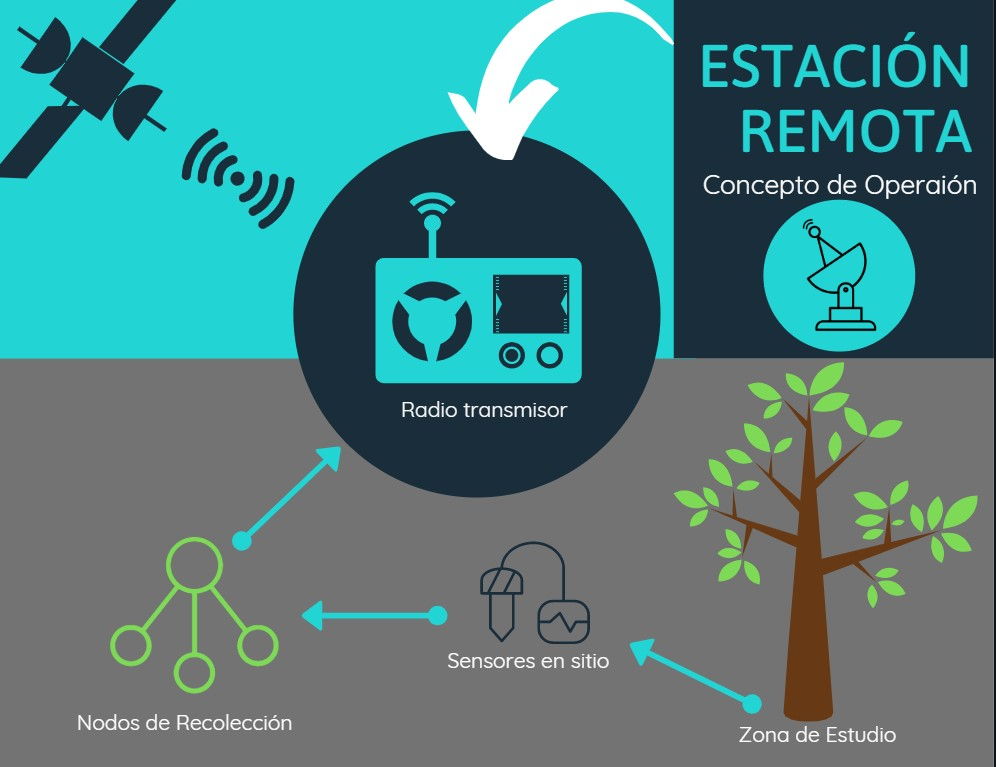
\includegraphics[scale=0.37]{Figuras/concepto_de_operacion_1.jpg}
\caption{Concepto de Operación para una estación Remota}
Elaboración Propia
\label{concepto de operacion}
\end{figure}

El concepto mostrado en la figura 1.1 fue el utilizado para la estación remota de la misión espacial Irazú; dicho concepto será el mismo para la nueva misión GWSat, esto incluye también, que el radio transmisor será reutilizado; por lo que conviene analizar los problemas operativos que surgieron en la misión Irazú como un antecedente, especialmente los que se dieron en la estación remota. Como antes se mencionó dentro de esta estación se encuentran los componentes electrónicos que hacen posible la transferencia de datos con el satélite, para el caso de la misión Irazú se identificaron tres problemas generales:

\begin{itemize}
    \item Ingreso de insectos y animales dentro del gabinete, por lo que no se garantizaba la protección de los componentes electrónicos internos.
    \item Incremento excesivo en la temperatura del radio transmisor.
    \item Fallos reiterados en la fuente de poder utilizada para el radio transmisor
    \item Pérdida de información debido al fallo general en la transmisión.
\end{itemize}

Como parte del problema, los responsables de la estación remota, identificaron como principal fuente de calor el radio transmisor; cabe resaltar que hasta ese momento, dentro del diseño inicial no se contempló ni se analizó la necesidad de un control térmico tanto para el radio como para el gabinete, por lo que para esta primera misión se encontraron desprovistos del mismo. Fuera de la información ya suministrada no se cuenta con documentación formal referente al estado operativo de la estación remota ni del radio transmisor durante la misión, ni reportes oficiales de reparaciones y mantenimientos realizados de los cuales se pudiera obtener información relevante para el proyecto.

\subsection{Requerimientos del Laboratorio}
En términos generales los requerimientos a nivel térmico-mecánico  por parte del laboratorio para la nueva misión GWSat se puede sintetizar en:
\begin{itemize}
    \item Determinar las condiciones térmicas del radio transmisor.
    \item Mantener el radio transmisor en condiciones operativas dentro del gabinete.
    \item Mantener una condición de estanqueidad en el gabinete de manera que no se permita el ingreso de polvo, agua, animales e insectos dentro del mismo.
    \item Considerar las condiciones climatológicas de Palo Verde en la determinación de los parámetros operativos de la estación.
    \item Poder introducir el radio transmisor dentro del gabinete desprovisto de su estructura termo-mecánica de fábrica.  
\end{itemize}

\section{Metodología}
\begin{figure}[h]
\centering
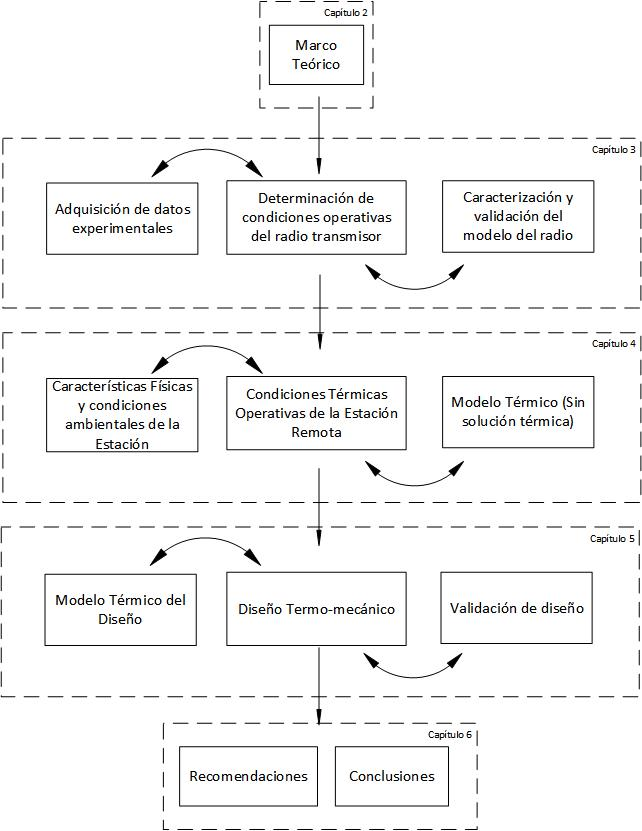
\includegraphics[width=0.9\linewidth]{Figuras/Metodologia.jpg}
\caption{Metodología de investigación}
Elaboración Propia
\label{Metodologia}
\end{figure}

Esta sección es una recopilación de lo más importante mediante los capítulos que definen los ejes centrales a seguir en el proyecto.

\begin{itemize}
    \item Capítulo 2: Hace referencia a toda la documentación técnica para la realización del diseño final.
    \item Capitulo 3: Se dedica exclusivamente al estudio del radio transmisor, con el fin de determinar su comportamiento térmico y la manera de poder analizarlo
    \item Capítulo 4: Involucra lo relacionado con la determinación de las condiciones térmicas, que determinarán los parámetros de diseño; y a las cuales la estación y el gabinete estarán sometidos.
    \item Capítulo 5: Se relaciona específicamente con el diseño en sí del control térmico, desde dos vertientes; la arquitectura de control térmico y la comparación con el modelo teórico propuesto.
    \item Capítulo 6: Dedicado a las conclusiones obtenidas del proceso de diseño, así como a las recomendaciones pertinentes sobre lo observado.
\end{itemize}

\subsection{Diseño de Investigación}

La investigación se define como experimental, ya que existe la posibilidad de la manipulación de la o las variables independientes haciendo variar por causa y efecto la variable dependiente \cite{meto}. En este caso el objetivo principal de la experimentación es la de caracterizar térmicamente el comportamiento del radio.

Al realizarle un análisis al funcionamiento del radio, además de las consultas realizadas a los encargados de la programación del mismo se identificaron tres posibles variables independientes que intervienen en la transmisión de datos por parte del radio hacia el satélite, que pudieran causar el aumento excesivo de la temperatura; sin embargo el criterio de selección y la especificación de dichas variables se realizará en el momento de definir el montaje del experimento.

\subsection{Enfoque de la Investigación}

Por las características propias del proyecto y de los objetivos planteados el enfoque de la investigación es cuantitativo por cumplir con las principales fases de este enfoque, las cuales se mencionan a continuación: \cite{meto}

\begin{itemize}
    \item Planteamiento del Problema.
    \item Revisión de la literatura y desarrollo del marco teórico.
    \item Desarrollo del diseño de investigación.
    \item Definición y selección de la muestra. 
    \item Recolección de datos.
    \item Análisis de datos.
    \item Reporte de Resultados.
\end{itemize}

\subsection{Definición del alcance de la investigación}

El principal  alcance de la investigación es de carácter exploratorio, ya que el tema no ha sido abordado antes  y actualmente se desconoce la magnitud del problema, al grado de que no se cuente con información necesaria para el planteamiento de una hipótesis. Sin embargo, una vez realizada la etapa exploratoria  referente al comportamiento térmico del radio, se pretende tener un alcance correccional donde se establezca el impacto de las variables independientes sobre el problema en estudio. \cite{meto}


% \pagenumbering{arabic}
% \chapter{Marco Teórico}

La presente sección tiene como objetivo realizar una presentación ordenada de la literatura que respalde el trabajo realizado: para lo cual se divide en cuatro áreas principales tal y como se observa en la Figura \ref{marco}. En la Sección 2.1 se abordan conceptos generales eléctricos, específicamente los relacionados con los elementos utilizados en circuitos de potencia presentes en el radio que permita comprender la naturaleza del problema térmico que presenta el dispositivo. Para el caso de la Sección 2.2 se abordan aspectos relacionados con los métodos de modelado térmico que se pueden realizar, así como las consideraciones para la resolución del problema planteado. En la Sección 2.3 se trata lo referente a las consideraciones para la resolución del proyecto, también se presenta los aspectos propios del diseño de las soluciones termo-mecánicas pasivas debido a la relación bidireccional que presentan estos dos aspectos. 

\begin{figure}[H]
\centering
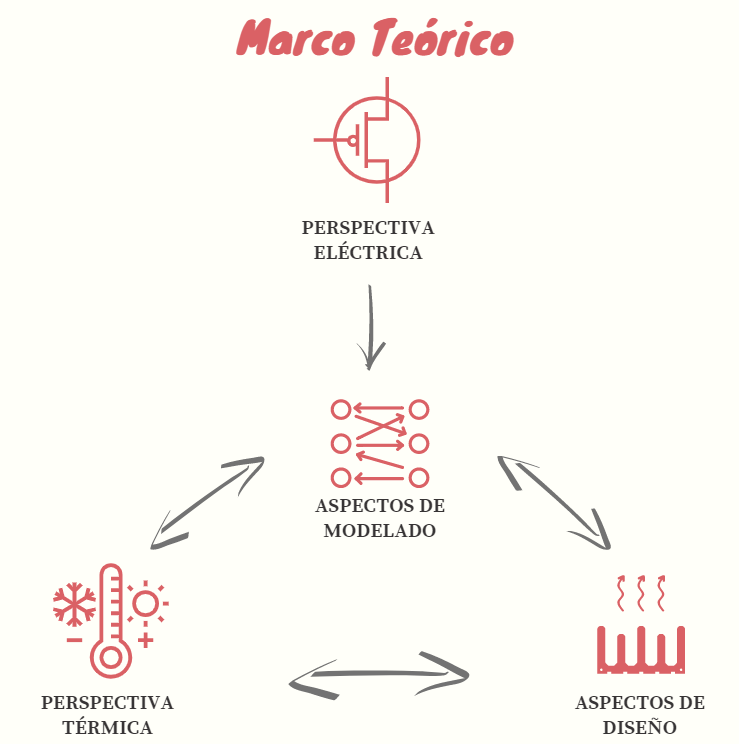
\includegraphics[scale=0.45]{Figuras/Marco_teorico.png}
\caption{Esquema de marco teórico}
Elaboración Propia
\label{marco}
\end{figure}


\section{Perspectiva Eléctrica}

Desde el siglo XIX, el físico inglés James Joule se dedicó al estudio de los efectos caloríficos producidos por el flujo de energía a través de diferentes medios; para lo cual realizó diferentes experimentos de los que obtuvo las siguientes conclusiones: \cite{joule}

\begin{enumerate}
    \item En un conductor, el flujo de la corriente eléctrica produce calentamiento.
    \item El incremento en la temperatura debido al flujo de corriente a través de un conductor, es proporcional al tiempo que dure dicho flujo de corriente.
    \item El aumento de la temperatura varía en relación con la intensidad de la corriente.
    \item El calentamiento es proporcional a la resistencia del conductor.
\end{enumerate}

Basado en estas observaciones postuló la siguiente Ley \cite{joule}:

\begin{center}

\centering
\textit{ La cantidad de calor producido por un conductor eléctrico es directamente proporcional al cuadrado de la intensidad ($I^2$), al valor de la resistencia del conductor y al tiempo, en segundos, durante el cual circule la corriente.}

\end{center}

Los dispositivos eléctricos, principalmente los de potencia, no escapan de los principios de esta ley, por lo que el aumento de temperatura debido a los flujos de corrientes que manejan, los ciclos de trabajo a los que son sometidos y el rápido avance de la tecnología junto con la necesidad de sistemas más eficientes y económicos, han tenido un impacto especialmente reflejado en el tamaño de los componentes electrónicos, además han provocado que la comprensión de la transferencia de calor en la cual se estudia el punto de equilibrio del medio continuo pierda validez a nano-escala, y el tamaño del dispositivo, junto con el tiempo pasen a ser determinantes como sucede en el caso de los IGBT y los MOSFET. \cite{cengel} 

\subsection{Semiconductor:}

Estos elementos pueden realizar la función de conductor o aislante de una manera selectiva según condiciones externas como campos electromagnéticos, campos eléctricos y radiación que determinan si dicho elemento se comporta como un circuito abierto o como un circuito cerrado. Dentro de los posibles elementos utilizados para la fabricación de semiconductores los más utilizados por la industria de componentes eléctricos son el Silicio (Si) y el Germanio (Ge) a los cuáles se les introduce partículas de otros elementos para convertirlos en semiconductores.\cite{beltran}
\\
Según el tipo de impureza que se introduzca, se puede obtener: 

\begin{itemize}
    \item Tipo N: poseen impurezas pertenecientes al grupo Va (Fósforo) lo que se traduce en un excedente de electrones libres.
    \item Tipo P: Sus impurezas son pertenecientes a compuestos del grupo Illa (Cadmio, Boro, entre otros) lo que provoca, debido a la falta de electrones, un exceso de cargas positivas.
\end{itemize}

En ambos casos el componente semiconductor es el encargado de realizar la conmutación de la señal eléctrica y existen dos principales tipos, el transistor unipolar o conocido por sus siglas en ingles FET (field-effect-transistor) y el transistor bipolar; su diferencia radica en que para el primero la activación del terminal de control se realiza aplicando tensión entre la puerta y la fuente, mientras que en el segundo se realiza inyectando corriente en la base que regula la conmutación.

\subsection{Tipos de semiconductores}

\textbf{MOSFET:} Su nombre proviene del acrónimo en ingles Metal-oxide-semiconductor-field-effect y su principio de funcionamiento consiste en aplicar tensión en la puerta (Gate) para que los electrones se muevan a la parte de abajo en la zona n+ en donde la tensión provoca que se genere un flujo de electrones que une las dos zonas conductoras llamadas fuente (Source) y Drenaje (Drain), para permitir el paso de la corriente \cite{beltran}. En la  Figura \ref{tipo n} se observa como, cuando se aplica un voltaje en la compuerta mayor a \SI{0}{\volt} y mayor que el voltaje de umbral se establece un puente de electrones entre la compuerta fuente y la compuerta de drenaje.

Los MOSFET son utilizados en aplicaciones de bajo voltaje ($<$\SI{250}{\volt}), baja potencia y altas frecuencias ($>$ \SI{200}{\kilo\hertz}), esto debido a la forma en que tienen pérdidas, tema que se tratará más adelante; sin embargo, se debe mencionar que en el caso de los MOSFET, las principales pérdidas  se deben a conducción y/o conmutación, estas últimas son las más bajas. \cite{beltran}

\begin{figure}[H]
\centering
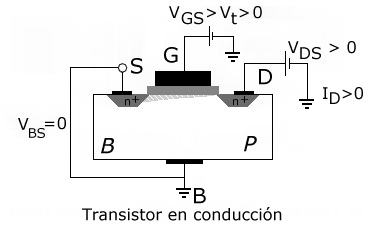
\includegraphics[scale=1]{Figuras/mosfet.png}
\caption{MOSFET tipo N en estado de conducción}
Fuente: \cite{Imagen_mosfet}
\label{tipo n}
\end{figure}

\textbf{BJT:} Utilizados principalmente en amplificadores los transistores de unión bipolar tienen un funcionamiento similar al MOSFET con la principal diferencia de que en este caso la conmutación se realiza al inyectar corriente en la base. Otra característica es que se encuentran construidos por tres piezas semiconductoras las cuales se disponen en dos posibles configuraciones: NPN o PNP . 

\begin{figure}[h]
\centering
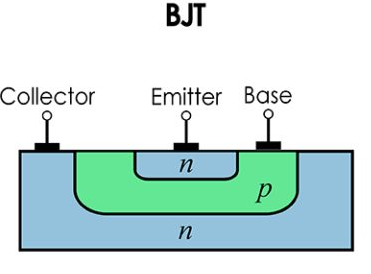
\includegraphics[scale=0.7]{Figuras/bjt.png}
\caption{BJT tipo NPN}
Fuente: \cite{bjt}
\label{bjt}
\end{figure}

\textbf{IGBT:} La interpretación del acrónimo es Insulated-gate bipolar transistor. Su principio de funcionamiento es similiar al de un MOSFET con la diferencia de que en este caso se agrega una capa p+ adicional la cual inyecta huecos en la capa n- y provoca una reducción en la caída de voltaje en la conducción; esto es motivo de reducción de las pérdidas por el mismo motivo, en consecuencia, son utilizados en aplicaciones de alto voltaje ($>$\SI{1000}{\volt}), bajas frecuencias en conmutación ($<$\SI{20}{\kilo\hertz}) y alta potencia. Sus características de construcción no permiten la conducción de corriente en modo inverso, por lo que a diferencia de otros transistores no requiere de un diodo intrínseco.\cite{beltran}

\begin{figure}[h]
\centering
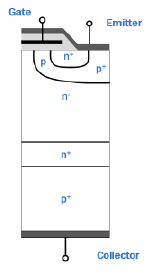
\includegraphics[scale=0.9]{Figuras/igbt.png}
\caption{IGBT tipo n}
Fuente: \cite{beltran}
\label{igbt}
\end{figure}

\subsection{Pérdidas en Semiconductores:}

En esencia los transistores son interruptores dentro de un circuito de potencia, por lo que se presentan pérdidas cuando el transistor se encuentra en estado de conducción y pérdidas cuando el mismo realiza la conmutación entre un estado y otro.

\textbf{Pérdidas por Conmutación:} Como su nombre lo sugiere estas pérdidas se dan en el momento en que el componente se apaga y enciende, produciéndose dichas pérdidas en el lapso que el componente tarda en responder al pasar de un estado a otro.\cite{beltran} 

\begin{figure}[h]
\centering
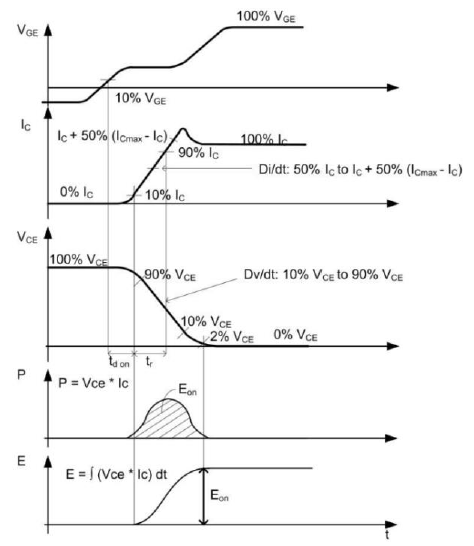
\includegraphics[scale=0.65]{Figuras/on.png}
\caption{Transistor en transición de encendido}
Fuente: \cite{beltran}
\label{encendido}
\end{figure}

Tal y como se observa en la Figura \ref{encendido} la energía que se pierde durante la conmutación de encendido del componente se cuantifica desde el momento que se da un flujo del \SI{10}{\percent} de la corriente de conducción hasta llegar a un \SI{90}{\percent} de la misma.   

\begin{figure}[H]
\centering
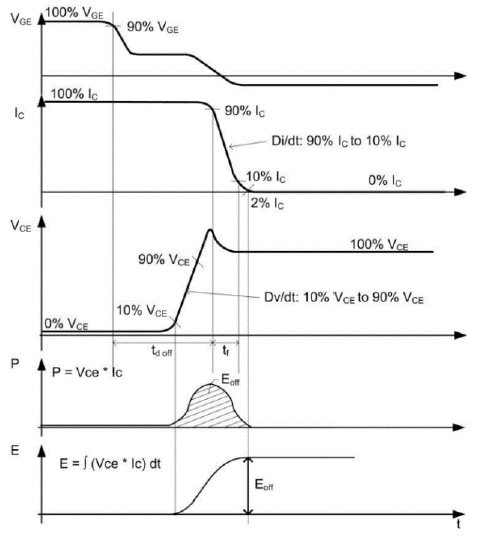
\includegraphics[scale=0.65]{Figuras/off.png}
\caption{Transistor en transición de apagado}
Fuente: \cite{beltran}
\label{apagado}
\end{figure}

Para el caso del estado transitorio de apagado en la Figura \ref{apagado} se observa que el tiempo que se considera para el cálculo de la pérdida de energía se cuenta desde el momento en que la caída de tensión representa un \SI{10}{\percent} del valor nominal hasta el momento en que la corriente de conducción alcanza un \SI{2}{\percent} de su valor nominal.

\textbf{Pérdidas por Conducción:} Se define como la energía disipada en forma de calor durante el tiempo en el que el componente, en este caso el transistor, se encuentra en estado de conducción \cite{beltran}. En este punto es importante resaltar que dichas pérdidas de potencia se pueden relacionar con la temperatura de unión como se muestra en la Ecuación \ref{pconduccion}, en donde las pérdidas por conducción son una función dependiente de la corriente de conducción y la temperatura de junta.

\begin{equation}\label{pconduccion}
    P_{cond} = f(I_{c},T_{j})  
\end{equation}

\section{Perspectiva de Modelado}

Una definición formal de modelo es la de ``esquema teórico, por lo general de carácter matemático, de un sistema o de una realidad compleja, que se elabora para facilitar su comprensión y el estudio de su comportamiento"\cite{rae}. En otras palabras un modelo es una forma de representación simplificada de la realidad o bien de un problema complejo que requiere de análisis, el cual por lo general se realiza a través de lenguaje matemático. Ahora bien en el momento que dicho lenguaje matemático es utilizado para describir un fenómeno o situación de naturaleza no matemática es donde se introduce el término de modelo matemático. \cite{morten}

Los modelos como tales pueden tener dos propósitos generales, uno de carácter descriptivo y otro de carácter predictivo, este último es mucho más complicado epistemológicamente ya que implícitamente requiere de supuestos o hipótesis que relacionen dos situaciones  diferentes pero con ciertas similitudes que los correlaciona: por un lado la situación que estima las características propias del fenómeno y por otro relacionan los condicionantes que permiten predecir el comportamiento de futuras situaciones. En el caso de un modelo descriptivo, si bien es cierto implica la definición de las características propias del fenómeno, dicha información es utilizada para análisis de un hecho ya ocurrido con diferentes propósitos. \cite{morten} 

Desde un punto de vista general, la literatura describe una serie de flujo de procesos para la realización de un modelo matemático, y aunque ciertas etapas del proceso varían el orden a seguir entre un autor y otro, se pueden resumir las etapas de la siguiente manera: \cite{morten}, \cite{comillas}

\begin{enumerate}
    \item Formulación del problema: Trata de la recolección y análisis pertinente de la información relevante que defina de una manera más precisa la situación que se requiere resolver, en este punto es donde también se plantean los supuestos y se recolectan los datos que más adelante deberán ser validados.
    \item Sistematización y formulación matemática: Consiste en la selección de las relaciones y objetos relevantes en el dominio de la investigación de manera tal que permita realizar una idealización del problema cuando se establecen las variables, parámetros y ecuaciones matemáticas que describen el problema
    \item Resolución: Hace uso de métodos matemáticos mediante la implementación de un algoritmo de obtención numérica óptima o cuasi-óptima con el objetivo de llegar a resultados matemáticos y conclusiones.
    \item Evaluación de la validez del modelo por comparación de datos: En este punto los resultados obtenidos de la resolución se deben comparar con los datos observados o predichos, con el conocimiento teórico o con la experiencia personal o compartida sin embargo, se debe aclarar que en el caso (el ideal) de validar el modelo en comparación con datos, los mismos no pueden ser los utilizados para la construcción del modelo ya que la intención de esta etapa, como su nombre lo indica, es determinar la utilidad del modelo para la descripción del fenómeno.
    \item Interpretación de los resultados y conclusiones: Una vez se tiene un modelo válido, del mismo se puede obtener información que permita sacar conclusiones y tomar decisiones respecto al fenómeno o situación estudiada según los propósitos planteados en la identificación del problema. 
    \item Implantación, documentación y mantenimiento: Esta etapa implica un cierre del ciclo de modelado, en el cual, una vez se tienen los resultados óptimos del modelo, la documentación necesaria permanece para garantizar la amplia difusión del modelo, así como sus posteriores correcciones.
\end{enumerate}

Es importante aclarar que las etapas antes descritas, lejos de ser un proceso lineal, son un constante ciclo en donde un modelo o sistema matemático se va adaptando a la interpretación del mundo real, en última instancia son el problema y la comprensión del mismo en la realidad los que definen los pasos a seguir para realizar un modelo que lo represente \cite{morten}. Por otro lado los pasos 4 y 5 suelen ser un motivo de discrepancia entre los autores ya que según la literatura consultada, dichas etapas suelen encontrarse invertidas, realizándose una interpretación de los resultados antes de la validación, pero como ya se mencionó la naturaleza misma del modelo determinará el orden de las etapas.

Es por ello que existen múltiples técnicas de modelado, mas aún con las herramientas de programación y software CAD 3D que permiten realizar modelos matemáticos de gran complejidad. En el caso de dispositivos electrónicos existe amplia literatura que describe diferentes tipos de modelos que caracterizan el comportamiento térmico de estos dispositivos a través de circuitos RC equivalentes. Los arreglos más comunes son las redes de Cauer y Foster. \cite{realtime}

\begin{figure}[H]
\centering
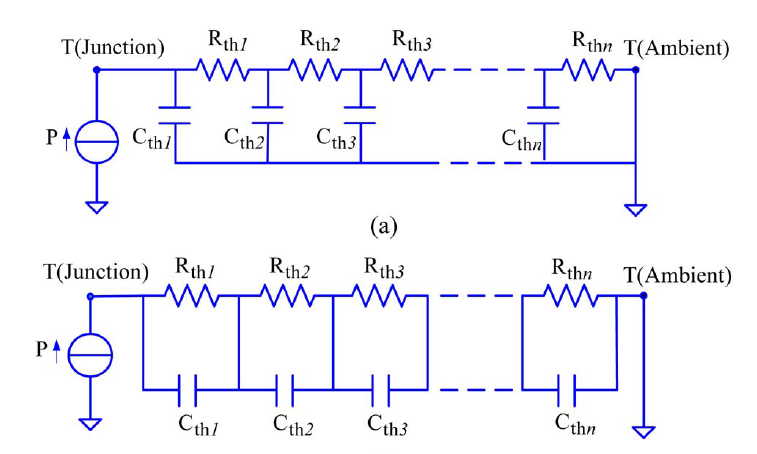
\includegraphics[scale=0.65]{Figuras/foster.png}
\caption{Red de Cauer y Foster respectivamente}
Fuente: \cite{realtime}
\label{foster}
\end{figure}

En la Figura \ref{foster} se observan dos configuraciones típicas que permiten simular un dispositivo de potencia  para determinar la temperatura de unión; en el caso de la red de Cauer describe el comportamiento térmico a lo largo de las capas constructivas del dispositivo, pero tiene la desventaja de tener una compleja implementación; por otro lado la red de Foster es de fácil implementación sin embargo, no predice el comportamiento térmico de sus capas constructivas. \cite{realtime}

Tomando como referencia la red de Foster, se puede obtener una impedancia térmica del sistema tal y como se muestra:

\begin{equation}\label{2}
    Z_{th}(t)=\sum ^{n}_{i=1}R_{i}\left ( 1-e\frac{t}{R_{i}C_{i}} \right )
\end{equation}

Donde $Z_{th}(t)$ es a lo que se conoce como  impedancia térmica, $R_{i}$ y $C_{i}$ son las resistencia y capacitancia térmica respectivamente de cada nodo de la red de Foster (figura \ref{foster}). La obtención de $Z_{th}(t)$ se puede realizar mediante una curva de mejor ajuste para obtener los valores de  $R$ y $C$  por medio de un software y con datos obtenidos a través de la experimentación. \cite{alfaro} 

\subsection{Red Generalizada}

Por otra parte, la Figura \ref{foster}  permite introducir el concepto de red generalizada, la cual es una extensión de las propiedades y teoremas de las redes eléctricas mediante la interconexión de elementos y fuentes generalizadas; para lo cual se utilizan  los conceptos de transvariable \( (\upsilon) \) y pervariable (f), donde la transvariable  requiere de dos puntos para medirse y se obtiene a través de los elementos, mientras que la pervariable se propaga por los elementos y su medición solo requiere de un punto. \cite{alfaro} 

Lo antes descrito se puede representar gráficamente de la siguiente manera:

\begin{figure}[H]
\centering
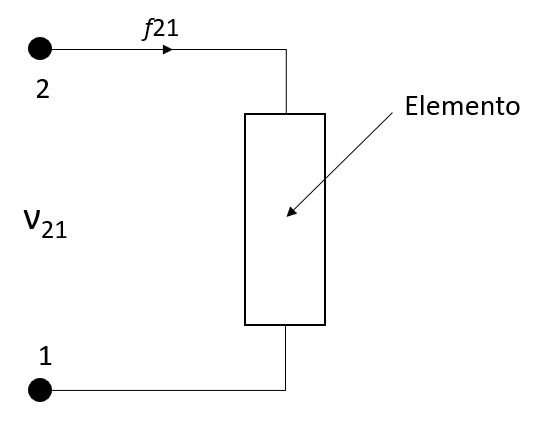
\includegraphics[scale=0.45]{Figuras/red.png}
\caption{Esquema de la Red Generalizada}
Fuente: Elaboración propia
\label{red}
\end{figure}


Por lo que el flujo de potencia que entra desde el punto 2 hacia el 1 se describe como \cite{alfaro}:

\begin{equation}\label{3}
    P(t) = f_{21}(t)\cdot \upsilon _{21}(t)
\end{equation}

En la Figura \ref{red} el ``Elemento'' adquiere su respectivo equivalente generalizado, dentro del circuito según se requiera para describir el sistema, como por ejemplo, puede ser reemplazado por un resistor generalizado, capacitor generalizado o bien incluso tener una fuente ideal de pervariable o transvariable. Para el caso de los sistemas térmicos se presentan a continuación los conceptos equivalentes dentro de la red generalizada:

\begin{table}[H]
\centering
\caption{Elementos generalizados para la representación de sistemas térmicos \cite{alfaro}}
\label{tab:2}
\begin{tabular}{@{}ccccc@{}}
\toprule
\textbf{\begin{tabular}[c]{@{}c@{}}Pervariable\\ ($f$)\end{tabular}} &
  \textbf{\begin{tabular}[c]{@{}c@{}}Integral de\\ Pervariable\\ ($h$)\end{tabular}} &
  \textbf{\begin{tabular}[c]{@{}c@{}}Transvariable\\ ($\upsilon$)\end{tabular}} &
  \textbf{\begin{tabular}[c]{@{}c@{}}Capacitor \\ Generalizado\\ ($C_{g}$)\end{tabular}} &
  \textbf{\begin{tabular}[c]{@{}c@{}}Resistor \\ Generalizado\\ ($R_{g}$)\end{tabular}} \\ \midrule
\begin{tabular}[c]{@{}c@{}}Flujo de calor\\ ($q$)\end{tabular} &
  \begin{tabular}[c]{@{}c@{}}Calor \\ ($H$)\end{tabular} &
  \begin{tabular}[c]{@{}c@{}}Diferencia de\\ Temperatura\\ ($\Delta T$)\end{tabular} &
  \begin{tabular}[c]{@{}c@{}}Capacitor \\ Térmico\\ ($C_{t}$)\end{tabular} &
  \begin{tabular}[c]{@{}c@{}}Resistor \\ Térmico\\ ($R_{t}$)\end{tabular} \\ \bottomrule
\end{tabular}
\end{table}

\subsubsection{Función de Transferencia}

Se define como una expresión matemática que relaciona y caracteriza una condición de entrada $u(t)$ con una condición de salida $y(t)$ en donde ambas están relacionadas mediante una ecuación diferencial para un sistema o proceso en específico. \cite{transferencia}

\begin{equation}\label{4}
    a_{0}y(t)+ a_{1}\frac{dy(t)}{dt}+\cdots+a_{n}\frac{d^{n}y(t)}{dt}=b_{0}u(t)+b_{1}\frac{du(t)}{dt}+\cdots +b_{n}\frac{d^{n}u(t)}{dt}
\end{equation}
\\
Representado a manera de bloques queda tal y como se muestra a continuación, donde se logra apreciar que la salida es dependiente de la entrada:

\begin{figure}[H]
\centering
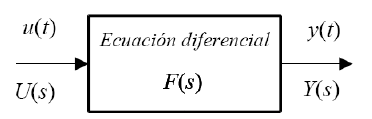
\includegraphics[scale=0.8]{Figuras/f.png}
\caption{Diagrama de entrada y salida de un sistema}
Fuente:\cite{transferencia}
\label{trans}
\end{figure}

Para lograr obtener la función de transferencia se recurren a las transformadas de Laplace, la cual es muy utilizada en aplicaciones ingenieriles en donde se presentan problemas con discontinuidades, o bien el comportamiento del sistema es periódico pero no fácilmente describible mediante expresiones matemáticas comunes.
\begin{equation}\label{laplace}
    F(s)=\pounds (f)=\int_{0}^{\infty }e^{-st}f(t)dt
\end{equation}

La transformada de Laplace básicamente consiste en tomar una ecuación diferencial y transformar cada derivada en un simple producto por $s$ y a la ecuación diferencial en $t$, en una ecuación algebraica en cuestión del termino complejo $s$ que define los polinomios: \cite{transferencia}

\begin{equation}\label{poli1}
    A(s)=\sum_{i=0}^{\infty }a_{i}s^{i}
\end{equation}

\begin{equation}\label{poli2}
 B(s)=\sum_{i=0}^{\infty }b_{i}s^{i}
\end{equation}

Por lo que, si se observa la Figura \ref{trans}, una vez que se obtienen las transformadas de ambos miembros de la ecuación se tiene que:

\begin{equation}
    Y(s)A(s) = U(s)B(s)
\end{equation}

Si se coloca la salida como la entrada multiplicada por el cociente de los polinomios \ref{poli1} y \ref{poli2}, donde a dicho cociente se le conoce como función de transferencia $F(s)$: \cite{transferencia}

\begin{equation}
    Y(s)A(s) = U(s)F(s)
\end{equation}

Donde:
\begin{equation}
F(s)=\frac{B(s)}{A(s)}
\end{equation}

Ahora bien, para utilizar el método se debe tener en consideración lo siguiente:\cite{transferencia}

\begin{itemize}
    \item La función de transferencia es aplicable exclusivamente a sistemas lineales e invariantes en el tiempo, por lo que en ocasiones se requiere de una linealización previa para implementar el método. Para que un sistema sea lineal, es importante recordar que debe cumplir con el principio de superposición y homogeneidad.
    \item En una función de transferencia el numerador es de orden menor o igual al del denominador, lo cual sucede siempre en sistemas físicos y se asumirá de manera implícita.
    \item A las raíces del denominador ($A(s)$) se le conocen como polos y estos determinan la estabilidad de la función; por otra parte a las raíces del numerador ($B(s)$) se le denominan ceros de $F(s)$.
    \item Sistemas que son físicamente distintos pueden tener la misma función de transferencia es decir, la función de transferencia caracteriza la dinámica del sistema, mas no proporciona información respecto a la estructura física real del sistema. 
\end{itemize}

\section{Perspectiva Térmica y de Diseño}
\textbf{Transferencia de Calor:} Se define como el proceso de propagación de calor en distintos medios, este se produce siempre que existe un gradiente térmico o cuando dos sistemas con temperatura diferente se ponen en contacto. El equipo de transferencia de calor, como los intercambiadores de calor están diseñados tomando en cuenta el análisis de la transferencia de calor. Los problemas de esta ciencia que se encuentran en la práctica se pueden considerar en dos grupos: 1) de capacidad nominal y 2) de dimensionamiento. Los problemas de capacidad nominal tratan de la determinación de la razón de la transferencia de calor, para un sistema existente a una diferencia específica de temperatura. Los problemas de dimensionamiento tratan con la determinación del tamaño de un sistema con el fin de transferir calor a una razón determinada para una diferencia específica de temperatura. \cite{cengel}

\textbf{Calor:} Se define como la forma de energía que se puede transferir de un sistema a otro como resultado de un diferencial de temperatura. \cite{cengel} 

\textbf{Calor Sensible:} Es la parte de la energía interna de un sistema asociada con el grado de actividad que sus moléculas tengan, entre mayor sea esta actividad mayor será el incremento de temperatura \cite{cengel}. También es el calor asociado a los cambios de temperatura de bulbo seco y dentro de las cargas térmicas que representan este tipo de energía interna, están las luces, componentes y dispositivos electrónicos así como motores eléctricos. \cite{apc}

\textbf{Calor Latente:} Esta asociado a la energía potencial interna de un sistema, por ende, hace referencia a la energía interna necesaria para vencer las fuerzas intermoleculares, lo que puede implicar cambios de fase \cite{cengel}. Por otra parte este calor se relaciona con la cantidad de humedad contenida en un cuerpo. \cite{apc}

\textbf{Mecanismos de transferencia de calor:} Existen tres mecanismos básicos.\cite{cengel}

\begin{itemize}
    \item Conducción: Transferencia de energía de las partículas más energéticas de una sustancia hacia las adyacentes, menos energéticas, como resultado de la interacción entre ellas.
    \item Convección: Transferencia de calor entre una superficie sólida y el líquido o gas adyacente que está en movimiento; y comprende los efectos combinados de la conducción y del movimiento del fluido
    \item Radiación: La energía emitida por la materia en forma de ondas electromagnéticas (o fotones), como resultado de los cambios en las configuraciones electrónicas de los átomos o moléculas.
\end{itemize}

\textbf{Convección natural:} Cuando la velocidad del fluido que está asociado a la transferencia de calor suele ser menore a \SI{1}{\meter/\second}, se habla de convección natural; en estos casos el coeficiente de transferencia por convección como está relacionado con la velocidad del fluido, suele ser muy bajo en comparación con los coeficientes de convección forzada. En estos casos  la diferencia de temperatura entre el medio y el objeto provoca transferencia de calor, por consiguiente, la temperatura del objeto decaerá un tanto y el fluido aumentará su temperatura en un tanto; esto provoca el efecto de flotación en donde la capa fina de aire que cubre el objeto caliente y que aumenta su temperatura, cambiará su densidad y se desplazará hacia las capas exteriores del fluido, el aire con una densidad menor y por ende una temperatura menor reemplazará la capa de aire caliente que se desplazó. Este proceso implica un movimiento del fluido y se repetirá hasta que el objeto caliente se encuentre en equilibrio térmico con el fluido. \cite{cengel}

\textbf{Convección natural sobre superficies:} Depende de la orientación y forma geométrica de la superficie, así como de las propiedades termofísicas del fluido. La resolución de problemas de convección natural sobre superficies en ocasiones se basa en estudios experimentales o bien en generalidades, ya que la dinámica del fluido es compleja y se dificulta la obtención de relaciones analíticas sencillas. \cite{cengel}

Cuando se determina el coeficiente promedio de convección, la velocidad de transferencia de calor por convección en una superficie sólida a temperatura uniforme $T_{s}$ circundante se puede determinar por medio de la ley de Newton del enfriamiento.\cite{cengel}

\begin{equation}\label{Newton}
    \dot{Q_{conv}}=hA_{s}(T_{s}-T_{\infty })\; \; (\si{\watt})
\end{equation}

Donde: 

\begin{itemize}
    \item \textit{h} es el coeficiente de transferencia de calor por convección natural (\si{\watt/\square\meter\celsius})
    \item $T_{\infty }$ es la temperatura del medio (\si{\celsius})
    \item$A_{s}$ es el área superficial de transferencia (\si{\square\meter})
\end{itemize}

\textbf{Determinación de coeficiente de convección natural:} Para el caso de una placa vertical de longitud $L$, de área superficial $A_{s}$ y suponiendo condiciones estacionarias de operación, además de considerar el aire como el gas ideal; el procedimiento para determinar el coeficiente de convección natural se define de la siguiente forma. \cite{cengel}

Se determina el número de Rayleigh considerando que para una placa en configuración vertical la longitud característica $L_{c}$ es igual a su longitud $L$.

\begin{equation}\label{ra1}
   Ra_{L}=\frac{g\beta (T_{s}-T_{\infty })L^{3}}{\nu^{2} }\;Pr
\end{equation}

Donde:

\begin{itemize}
    \item \textit{g} es la aceleración gravitacional (\si{\meter/\square\second})
    \item \textit{Pr} es el número de Prandtl 
    \item $\beta$ es el coeficiente de expansión volumétrica (\si{\kelvin})
    \item $\nu$ es la viscosidad cinemática del fluido (\si{\square\meter/\second})
\end{itemize}

Todas las propiedades termofísicas del aire se evalúan a la temperatura de película $T_{f}$, asumiendo 1 atm de presión.

\begin{equation}\label{tf}
   T_{f} = \frac{T_{s}+T_{\infty }}{2}\;\;(\si{\celsius})
\end{equation}

Para determinar el número de Nusselt se utiliza la expresión que aplica para todo el intervalo de $Ra$ la cual es compleja pero más exacta y la misma se utiliza para la configuración de placas verticales.

\begin{equation}\label{nu1}
   Nu=\left \{ 0.825+\frac{0.387Ra_{L}^{1/6}}{\left[ 1+(0.492/Pr)^{9/16}\right] ^{8/27}}\right\}^{2} 
\end{equation}

Una vez que se obtiene el número de Nusselt se puede obtener el coeficiente de convección natural.

\begin{equation}\label{h1}
    h=\frac{k}{L}Nu\; \; (\si{\watt/\square\meter\celsius})
\end{equation}

\textbf{Transferencia de calor a través de un recinto cerrado esférico:} Las corrientes de fluido o en este caso de aire resultantes de una transferencia de calor por convección natural, se vuelven relevantes cuando se trata de recintos cerrados, donde estas corrientes o desplazamientos del fluido no permanecen estacionarios y se establece un  movimiento de rotación dentro del recinto para mejorar la transferencia de calor. Las características de la transferencia de calor estarán estrechamente relacionadas con la posición de la fuente de calor interna, ya sea si la misma se encuentra arriba, en medio o abajo, para el caso de un recinto vertical; como se mencionó anteriormente el fluido más caliente buscará la parte superior por lo que si la fuente de calor se encuentra en la parte superior no se desarrollarían estas corrientes convectivas y se hablaría entonces de un caso de conducción pura. Es por ello que en ocasiones resulta de gran utilidad hacer la simplificación de asumir que la geometría del recinto y de la fuente de calor se presentan en una configuración de dos esferas concéntricas entre sí, para lo cual, el cálculo de transferencia de calor por convección natural dentro del recinto se puede expresar como: \cite{cengel}  

\begin{equation}\label{q2}
    \dot{Q} = k_{ef}\pi\left (\frac{D_{i}D_{e}}{L_{c}}\right )(T_{i}-T_{e}) \; \; \; (\si{\watt})
\end{equation}

Donde:

\begin{itemize}
    \item $D_{i}$ es el diámetro interno (\si{\meter})
    \item $D_{e}$ es el diámetro externo (\si{\meter})
    \item $T_{i}$ es la temperatura superficial interna (\si{\celsius})
    \item $T_{e}$ es la temperatura superficial externa (\si{\celsius})
    \item $k_{ef}$ es el coeficiente de conductividad térmica efectiva (\si{\watt/\meter\celsius})
\end{itemize}

Para este caso las propiedades termofísicas del aire se evalúan en lo que se define como $T_{prom}$

\begin{equation}\label{tprom}
    T_{prom} = \frac{T_{i}+T_{e}}{2}\;\;(\si{\celsius}) 
\end{equation}

La longitud característica se define de la siguiente manera para dos esferas concéntricas

\begin{equation}\label{lc}
    L_{c}=\frac{D_{e}-D_{i}}{2}\;\;(\si{\meter})
\end{equation}

El coeficiente de conductividad térmica efectiva se puede determinar mediante la siguiente expresión

\begin{equation}\label{kef}
    k_{ef}=0.74k\left ( \frac{Pr}{0.861+Pr} \right )^{1/4}(F_{esf}Ra_{L})^{1/4} \; \; (\si{\watt/\meter\cdot\celsius})
\end{equation}

Para la Ecuación \ref{kef} el valor de $Ra_{L}$ se determina mediante la Ecuación \ref{ra1}. En el caso de esferas concéntricas se utiliza el factor geométrico $F_{esf}$ que se define como

\begin{equation}\label{fesf}
    F_{esf}=\frac{L_{c}}{(D_{i}D_{e})^{4}(D_{i}^{-7/5}+D_{e}^{-7/5})^{5}}
\end{equation}

La relación para  $k_{ef}$ es válida para valores de {$0.70 \leq$ Pr $\leq 4200$}\; $\textrm{y}$ \; {$10^{2}\leq$ $F_{esf}Ra_{L}\leq 10^{4}$}.\;\; $\textrm{Si}$\;\;$k_{ef}/k<1$, se debe asumir que $k_{ef}=k$

\textbf{Determinación del coeficiente convección externa para una esfera:} A partir de las suposiciones de que existen condiciones estacionarias de operación, no se incluyen los efectos de la radiación, el aire es un gas ideal y a una atmósfera de presión, la temperatura de la superficie exterior de la esfera se mantiene uniforme en todo momento, por último para evaluación del coeficiente de transferencia de calor se toma la temperatura superficial de la esfera como constante, para evitar la complejidad de una variación en el coeficiente de convección debido a la variación de la temperatura superficial. Sin embargo, la viscosidad dinámica del aire $\mu _{s}$ debe ser evaluada a la temperatura promedio superficial. El procedimiento se describe a continuación. \cite{cengel}

El coeficiente de convección promedio se define como

\begin{equation}\label{hext}
    h=\frac{k}{D}Nu\; \; (\si{\watt/\square\meter\celsius})
\end{equation}

Donde el número de Nusselt es

\begin{equation}\label{nu2}
    Nu=2+\left [ 0.4\, Re^{1/2}+0.06\,Re^{2/3} \right ]Pr^{0.4}\left ( \frac{\mu _{\infty }}{\mu_{s}} \right )^{1/4}
\end{equation}

Donde:

\begin{itemize}
    \item $\mu _{\infty}$ es la viscosidad dinámica del aire evaluada a temperatura ambiente (\si{\kilo\gram/\meter\cdot\second}) 
    \item $\mu_{s}$ es la viscosidad dinámica del aire evaluada a temperatura superficial promedio (\si{\kilo\gram/\meter\cdot\second})
\end{itemize}

La Ecuación \ref{nu2} es válida para valores de 3.5 $\leq$ Re $\leq$ 80000 y 0.7 $\leq$ Pr $\leq$ 380

Para este caso el número de Reynolds es

\begin{equation}\label{re2}
    Re=\frac{VD}{\nu }
\end{equation}

Donde:

\begin{itemize}
    \item $V$ es la velocidad del fluido (\si{\meter/\second}) 
    \item $D$ es el diámetro de la esfera (\si{\meter})
\end{itemize}

\textbf{Determinación de la radiación para entre dos esferas concéntricas:} Al igual que la convección natural en recintos cerrados, la radiación es un factor significativo dentro de la transferencia de calor, por lo que la misma no se puede omitir. Los problemas relacionados con radiación suelen ser complejos, debido a que el fenómeno en sí es complicado de analizar mediante expresiones sencillas, por lo general se encuentran involucrados muchos factores que determinan el comportamiento térmico debido a este mecanismo de transferencia; es por ello que se suele recurrir a generalidades o simplificaciones cuando se resuelven problemas asociados a la radiación. Una de ellas es la utilización de geometrías sencillas como cilindros o esferas, habitáculos o recintos de pocas caras, principalmente por la complejidad que implica analizar los factores de visión entre las distintas superficies. Para  dos esferas concéntricas con radios $r_{1}$ y $r_{2}$ donde $r_{1}$ $<$ $r_{2}$, se puede obtener la siguiente expresión para la transferencia de calor.\cite{cengel}

\begin{equation}\label{radint}
    \dot{Q}_{12}=\frac{A_{1}\sigma (T_{1}^{4}-T_{2}^{4})}{\frac{1}{\varepsilon _{1}}+\frac{1-\varepsilon _{2}}{\varepsilon _{2}}\left | \frac{r_{1}}{r_{2}} \right |^{2}}\;\;(\si{\watt})
\end{equation}

Donde:

\begin{itemize}
    \item $\sigma$ es la constante de Stefan-Boltzmann (\num{5,67xe-8}\si{\watt/\square\meter\cdot\kelvin\tothe{4}})
    \item $\varepsilon _{1}$ es la emisividad de esfera 1
    \item $\varepsilon _{2}$ es la emisividad de esfera 2
\end{itemize}

\textbf{Cálculo de Radiación Solar:} El sol es la principal fuente de energía, la misma llega en forma de radiación. Esta energía solar que ingresa a la atmósfera terrestre se le conoce como irradiancia solar total $G_{sc}$ la cual se considera como la constante solar de valor. \cite{cengel}

\begin{equation}\label{gsc}
    G_{sc}=\SI{1373}{\watt/\square\meter}
\end{equation}

Esta constante solar representa la tasa a la cual la energía solar incide en el borde de la atmósfera en una superficie imaginaria perpendicular, cuando la Tierra se encuentra a su distancia media del Sol la cual varia aproximadamente un \SI{3,3}{\percent} durante el año. \cite{cengel}

De esa cantidad de radiación solar, se estima que una vez, dicha energía entra en la atmósfera, se distribuye aproximadamente de la siguiente manera. \cite{solar}

\begin{itemize}
    \item \SI{30}{\percent} es reflejada.
    \item \SI{17}{\percent} es absorbida por la atmósfera
    \item \SI{53}{\percent} llega a la superficie de la Tierra, la misma se subdivide en:
    \begin{itemize}
        \item \SI{31}{\percent} en radiación directa.
        \item \SI{22}{\percent} en radiación difusa.
    \end{itemize}
\end{itemize}

Se considera como radiación solar directa aquella que llega a la superficie terrestre sin cambio de dirección; la radiación refleja es aquella que una vez que tiene contacto con la superficie cambia su dirección y la radiación difusa es la que llega a la superficie luego de haber cambiado de dirección por las partículas en atmósfera. Por otro lado la distribución de la radiación antes mostrada, varia significativamente en función de múltiples factores como las condiciones meteorológicas presentes en el momento, posición de la Tierra con respecto al Sol y de igual manera, la posición del Sol con respecto a una posición geográfica en específico.\cite{solar}

La radiación incidente sobre una superficie completamente perpendicular a las ondas de radiación, justo en el exterior de la atmósfera varia aproximadamente \num{\pm45}\si{\watt/\square\meter} durante el año por lo que el cálculo de este valor depende del número de día del año y de la constante solar. \cite{solar}

\begin{equation}\label{gon}
    G_{on}=G_{sc}\left ( 1+0.033\cos \left ( \frac{360*n}{365} \right ) \right )\;\;(\si{\watt/\square\meter})
\end{equation}

Donde:

\begin{itemize}
    \item $n$ es el número del día en el año.
\end{itemize}

Partiendo de la suposición de un día claro, la radiación total recibida por una superficie horizontal es. \cite{solar}

\begin{equation}\label{radiacion total}
    G_{c}=G_{cb}+G_{cd}\;\;(\si{\watt/\square\meter})
\end{equation}

Donde:

\begin{itemize}
    \item $G_{cb}$ es la radiación directa (\si{\watt/\square\meter})
    \item $G_{cd}$ es la radiación difusa (\si{\watt/\square\meter})
\end{itemize}

La Ecuación \ref{radiacion total} se puede expresar de la siguiente manera

\begin{equation}\label{gc}
    G_{c}=(\tau _{b}+\tau _{d})\cdot G_{on}\cdot(\cos\varphi \cdot \cos\delta \cdot \cos\omega +\sin\delta \cdot \sin\delta ) 
\end{equation}

Donde:

\begin{itemize}
    \item $\varphi$ es la latitud
    \item $\delta$ es el ángulo de declinación
    \item $\omega$ es el ángulo horario
\end{itemize}

Para el caso de $\tau _{b}\; \textrm{y} \;\tau _{d}$ se deben realizar cálculos aparte tal y como se muestra

\begin{align}\label{tb}
    \tau _{b}&=a_{0}+a_{1}\cdot e^{(-k/\cos\theta _{z})}\\
    \tau _{d}&=0.271-0.294\cdot \tau _{b}
\end{align}

Nuevamente para el caso de la Ecuación \ref{tb} se deben realizar cálculos adicionales para las constantes $a_{0}\;,a_{1}\; \textrm{y}\; k$, por otra parte $\theta_{z}$ hace referencia al ángulo cenit.

\begin{align}
    a_{0}&=r_{0}\cdot (0.4237-0.00821\cdot (6-A)^{2})\\
    a_{1}&=r_{1}\cdot (0.5055-0.00595\cdot (6.5-A)^{2})\\
    k&=r_{k}\cdot (0.2711-0.01858\cdot (2.5-A)^{2})
\end{align}

Las constantes $r_{0}\;,\;r_{1}\;\textrm{y}\;r_{k}$, se obtienen a partir de la Tabla \ref{constantes solares}. Por otra parte el término $A$, es el área superficial sobre la cual se estima la incidencia de radiación solar.

\begin{table}[H]
\centering
\caption{Factores $r_{0}\;,\;r_{1}\;\textrm{y}\;r_{k}$, según el tipo de clima }
\label{constantes solares}
\begin{tabular}{lccc}
\toprule
\textbf{Tipo de Clima}     & \textbf{$r_{0}$} & \textbf{$r_{1}$} & \textbf{$r_{k}$} \\ \hline
Tropical                   & 0.95        & 0.98        & 1.02        \\
Verano de latitudes medias & 0.97        & 0.99        & 1.02        \\
Verano subártico           & 0.99        & 0.99        & 1.01        \\
Invierno latitudes medias  & 1.03        & 1.01        & 1           \\ \bottomrule
\end{tabular}
\end{table}

\textbf{Espaciamiento óptimo de las aletas para un sumidero de calor:} En el diseño o selección de un sumidero de calor, uno de los aspectos a considerar es el espaciado entre las aletas ya que el objetivo principal de un disipador o sumidero de calor es aumentar el área superficial de transferencia de calor, por lo que si el espaciado entre las aletas es muy reducido, se tiene un área superficial mayor sin embargo, se reduce el coeficiente de convección, debido a la resistencia entra  agregada al paso del fluido entre las aletas; por otra parte, si el espacio es amplio, se mejora el coeficiente de convección pero sacrifica el área superficial de transferencia\cite{cengel}. La recomendación típica es que cuando se utiliza disipación térmica pasiva, el espaciado entre las aletas sea amplio, mientras que para configuras de disipación activa se pueden realizar arreglos más densos de aletas. Para diseños mas precisos y optimizados existen distintas herramientas para la determinación de la topología de un sumidero; una de las opciones más accesibles es estimar el espaciado óptimo entre las aletas. \cite{cengel},\cite{topologia}

Para una configuración como la mostrada en la Figura \ref{ejemplo disipador}, el espaciado óptimo $S_{opt}$ se puede obtener de la siguiente manera, asumiendo $T_{s}=constante$. \cite{cengel}

\begin{figure}[H]
\centering
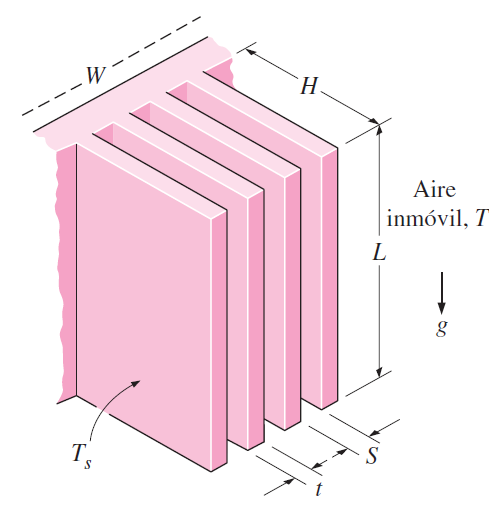
\includegraphics[scale=0.55]{Figuras/ejemplodisipador.png}
\caption{Esquema constructivo de un disipador de calor}
Fuente:\cite{cengel}
\label{ejemplo disipador}
\end{figure}

\begin{equation}\label{sopt}
    S_{opt}=2.714\cdot \frac{L}{Ra_{L}^{0.25}}\;\;(\si{\meter})
\end{equation}

Una vez con el espaciado óptimo se puede determinar el número de aletas para una configuración como la mostrada en la Figura \ref{ejemplo disipador}.

\begin{equation}\label{numeroaletas}
    n=\frac{W}{S+t}
\end{equation}

Cuando el espaciado $S$ es el  óptimo $S_{opt}$ el número de Nusselt es constante con un valor de 1,307; lo que permite determinar también el coeficiente de convección natural. 

\begin{equation}\label{hdisipador}
    Nu=\frac{hS_{opt}}{k}=1.307
\end{equation}

Finalmente para determinar la razón de transferencia de calor se utiliza la Ecuación \ref{Newton}, para el caso de $Ra_{L}$, se utiliza la Ecuación \ref{ra1}, se evaluán las propiedades del aire a $T_{prom}$ (Ecuación \ref{tf}).

\textbf{Refrigeración Pasiva versus Refrigeración Activa:} Se dice que la refrigeración es pasiva cuando la transferencia de calor se realiza de manera natural con los elementos del sistema sin necesidad de mecanismos o trabajo mecánico para acelerar o mejorar el proceso de transferencia, como sí sucede en el caso de la refrigeración activa donde existe un flujo forzado del medio refrigerante. \cite{cengel}

La refrigeración pasiva como no depende de mecanismos que requieren de energía para realizar el trabajo mecánico, así como equipos auxiliares que eventualmente requerirán de mantenimiento, reducen el costo y aumentan la confiabilidad del sistema; sin embargo, presenta la desventaja de ser eficiente para flujos de calor bajos e implica que el elemento a refrigerar opere a temperaturas mas altas. \cite{motor}

\textbf{Control térmico en gabinetes eléctricos:} Cuando se habla de circuitos y tableros eléctricos que se utilizan en múltiples áreas de la industria, se debe considerar que los mismos son susceptibles a diferentes factores que pueden provocar daños en su estructura y componentes; por lo que, actualmente en la industria existen diversas soluciones en forma de gabinetes y racks que aseguran la integridad de sus componentes internos\cite{factores}. Sin embargo, esto representa un reto a nivel térmico el poder mantener en temperaturas operativas a los componentes electrónicos; se estima que por cada \SI{10}{\celsius} por encima de la temperatura de operación del recinto se reduce hasta en un $50\%$ la vida útil del dispositivo electrónico. \cite{hoffman}

Por otro lado la humedad presente en los gabinetes eléctricos representan un riesgo muy grande para la integridad de los componentes internos, y que se podrían producir condensaciones internas debido al flujo de aire húmedo que choca contra superficies con una temperatura por debajo de la de rocío; y provocar daños en componentes electrónicos y posibles focos de corrosión en el gabinete y herrajes. Este problema se presenta principalmente en gabinetes que tiene un sistema de refrigeración robusto en donde el evaporador podría generar condensaciones a lo interno, o bien al realizar aperturas de mantenimiento, el ingreso de aire húmedo caliente con respecto al aire frió interno podría provocar la condensación. \cite{risoul}

Una forma de determinar si la condensación se producirá es mediante la Ecuación \ref{calculo td}  que permite relacionar la temperatura ambiente $T_{amb}$ con el porcentaje de humedad relativa $HR$ para obtener la temperatura de rocío $T_{d}$.\cite{td}

\begin{equation}\label{calculo td}
    T_{d}= c3*\frac{\ln \left ( \frac{RH}{100} \right )+\frac{c2*T_{amb}}{c3+T_{amb}}}{c2-\ln \left ( \frac{RH}{100} \right )-\frac{c2*T_{amb}}{c3+T_{amb}}}
\end{equation}

Para $T\,>0\degree C\;:\;c2=17,08085\;;\;c3=234,175$
% \chapter{Condiciones Operativas del Radio Transmisor}

El presente capítulo tiene como objetivo presentar el estudio realizado al radio transmisor, ya que para conocer su comportamiento térmico, se debía primero establecer que parámetros de funcionamiento tenían influencia en el comportamiento térmico del mismo, para luego caracterizar su comportamiento mediante un modelo que permitiera probar diferentes condiciones operativas y predecir su desempeño térmico. Para lo cual se sometió al radio a diferentes pruebas, con las cuales se pretendía obtener datos experimentales que permitieran conformar un modelo matemático a partir de dichos datos.

\section{Descripción General}

El radio transmisor en estudio es un KENWOOD modelo TM-D710A y sus principales características en valores nominales se muestran a continuación:\cite{manual}

\begin{table}[H]
    \centering
    \caption{\textbf{Características Eléctricas del Radio}}
    \begin{tabular}{cccc}
    \toprule
    \multicolumn{3}{c}{\textbf{Característica}} & \textbf{Magnitud}  \\
    \midrule
    \multicolumn{3}{c}{Voltaje} & \SI{13,8}{\volt} DC \num{\pm 15}\si{\percent} \\
    \midrule
    \multirow{6}{*}{Corriente} & \multirow{3}{*}{VHF} &  HI & Menor \SI{13}{\ampere} \\ && MID & Menor a \SI{5,5}{\ampere} \\ && LOW & Menor a \SI{4}{\ampere}\\
    & \multirow{3}{*}{UHF} &  HI & Menor a \SI{13}{\ampere}\\ && MID & Menor a \SI{6,5}{\ampere} \\ && LOW & Menor a \SI{5}{\ampere} \\
    \midrule
    \multicolumn{3}{c}{Rango de Temperatura de Operación} & De \SI{-20}{\celsius} a \SI{60}{\celsius}
    \\
    \midrule
    \multicolumn{2}{c}{\multirow{2}{*}{Masa (Aprox)}} & Panel de Operación & \SI{0,3}{\kilogram}\\
    && Unidad TX/RX & \SI{1,2}{\kilogram}\\
    \midrule
    \multicolumn{2}{c}{\multirow{3}{*}{Potencia de Salida RF}} & HI & \SI{50}{\watt}\\
    &&  MID & $\sim$\SI{10}{\watt} \\ && LOW & $\sim$\SI{5}{\watt} \\
    \bottomrule
    \end{tabular}
    \label{tab:1}
\end{table}

En la figura \ref{fotoradio} se observa que se trata de un radio transmisor de uso comercial, principalmente para transporte o automóviles, ya que el mismo cuenta con características como alertas del clima sin embargo, las mismas solo están disponibles en norteamerica. Es importante notar que el radio cuenta con tres partes externas principales: el micrófono, el panel frontal de control y la carcasa principal. Ni la imagen, ni lo antes descrito excluye el hecho de que para su correcto funcionamiento y dependiendo de la aplicación, el radio cuenta con otros elementos los cuales no se representan en la imagen.

\begin{figure}[H]
\centering
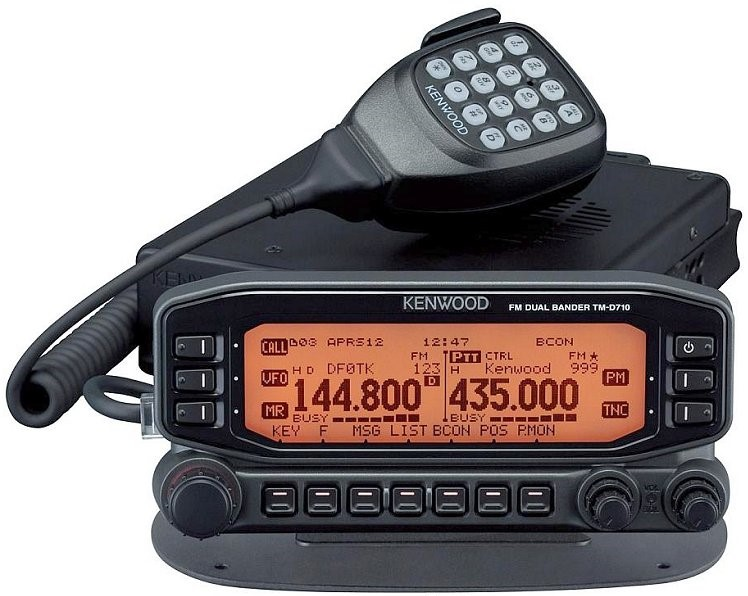
\includegraphics[scale=0.5]{Figuras/radio.jpg}
\caption{Radio KENWOOD TM-D710A}
Fuente:\cite{fotoradio}
\label{fotoradio}
\end{figure}

En síntesis, uno de los principales problemas, es implementar mecánica y térmicamente un radio de uso comercial, en un ambiente y aplicación no convencional o para lo cual no fue realmente diseñado; ya que de las partes antes descritas, es de especial interés, la carcasa principal, ya que la misma funciona como disipador térmico del radio, esto se convierte en un problema si la misma es retirada tal y como sucederá en la GRT, es decir, para lograr introducir el radio dentro de un gabinete en conjunto con otros elementos de la estación y optimizar el espacio, se debe desproveer el radio de todos aquellos elementos que no son estrictamente innecesarios. Para el caso particular de este radio el panel frontal de control no puede estar desconectado de la carcasa principal, ya que sin el radio no funciona, a pesar de que el mismo será operado remotamente; uno de los elementos que no estarán dentro de la estación es el micrófono que se observa en la Figura \ref{fotoradio}. 

\begin{figure}[H]
\centering
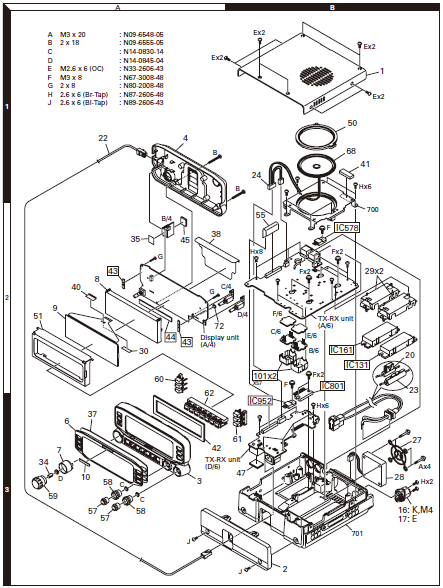
\includegraphics[scale=1.25]{Figuras/Despiece.png}
\caption{Despiece de Radio KENWOOD TM-D710A}
Fuente:\cite{manual}
\label{despiece}
\end{figure}

Como se observa en la Figura \ref{despiece}, el radio transmisor se trata de un dispositivo electrónico complejo, por lo que para realizar su análisis respectivo se consultó con los encargados del mismo y se llegó a las siguientes conclusiones preliminares:

\begin{itemize}
    \item El calor producido por el radio se concentra en el elemento TX-RX unit (A/6), lo que de ahora en adelante se conocerá como placa principal, y específicamente en los MOSFET de potencia marcados en la Figura \ref{despiece} como IC161 e IC131.
    \item El elemento descrito como TX-RX Unit (D/6), lo que de ahora en adelante se conocerá como placa secundaria se encuentra unida por dos puertos, uno de comunicación y otro de energía a la placa principal por lo cual dichos elementos no se pueden separar.
    \item El panel frontal de control deberá ir tal cual se muestra en en la Figura \ref{fotoradio} dentro del gabinete.
    \item El radio se despojará del micrófono y de elementos como el parlante (\#68) y los asociados al mismo.
    \item No se utilizarán en la estación de los elementos 1, 2 y 701 (Figura \ref{despiece}), de ahí es que surge la necesidad se implementar una solución mecánica para el soporte de la placa principal y secundaria.
\end{itemize}

\begin{figure}[H]
\centering
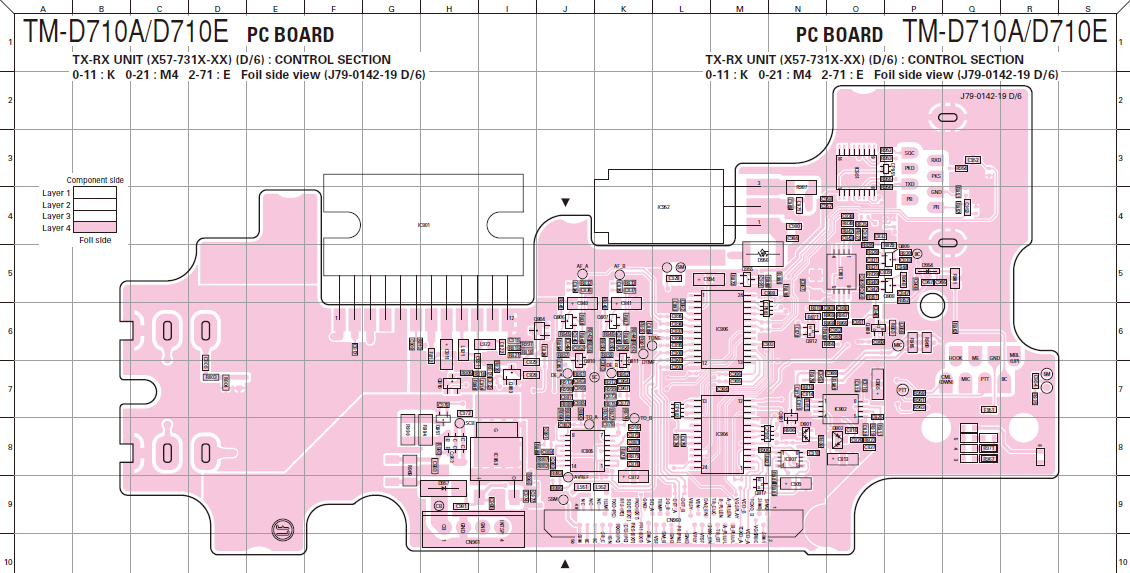
\includegraphics[scale=0.55]{Figuras/placasecundaria.png}
\caption{Plano de la PCB de la placa secundaria}
Fuente:\cite{manual}
\label{secundaria}
\end{figure}

\begin{figure}[H]
\centering
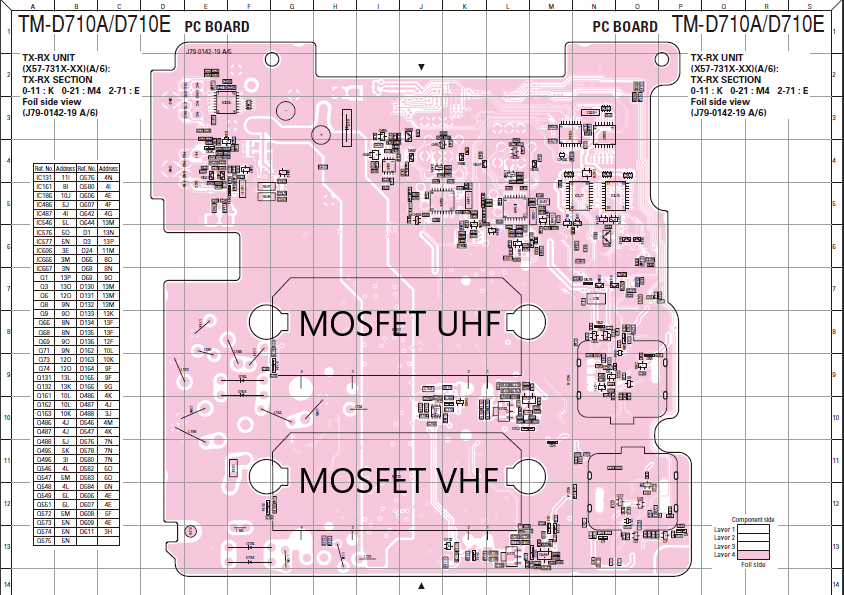
\includegraphics[scale=0.75]{Figuras/placaprincipal.png}
\caption{Plano de la PCB de la placa principal}
Fuente:\cite{manual}
\label{principal}
\end{figure}

En las Figuras \ref{secundaria} y \ref{principal} se presentan los planos de la tarjeta secundaria y principal respectivamente. En el caso de la placa principal se señala también los dos MOSFET de potencia que se identificaron como las fuentes de  calor a considerar, la más crítica el MOSFET de $UHF$, es el que mayor incremento de temperatura tendrá porque trabaja a una mayor frecuencia, además a pesar de tener dos canales de transmisión, simultáneamente solo se utilizará uno por lo tanto solo se estudiará el caso en el que la transmisión se realiza en $UHF$.

En cuanto al MOSFET de $UHF$ se tienen las siguientes características que se presentan en la Tabla \ref{mosfet}, de la cual cabe resaltar la temperatura de operación máxima que permite el dispositivo que junto con la temperatura máxima de operación del radio, establecen un parámetro que se debe cumplir dentro de la estación remota.  \cite{mosfet}

\begin{table}[H]
\centering
\caption{Características Generales del MOSFET de UHF}
\label{mosfet}
\begin{tabular}{lc}
\toprule
{\color[HTML]{000000} \textbf{Descripción}} & Silicon RF Power Modules \\
\textbf{Fabricante}                         & MITSUBISHI Electric      \\
\textbf{Número de parte}                    & RA60H4452M1              \\
\textbf{Código de Package}                  & H2M                      \\
\textbf{Rango de Frecuencia (\si{\mega\hertz})}          & 440-520                  \\
\textbf{Potencia Máxima (\si{\watt}})                & 60                       \\
\textbf{Voltaje de Alimentación (\si{\volt})}   & 12,5                     \\
\textbf{Temperatura de Operación (\si{\celsius})}      & -30 a 100                \\ \bottomrule
\end{tabular}
\end{table}

En el Apéndice \ref{anexo1} se muestra las características físicas del MOSFET de potencia, las cuales son características de un empaquetado tipo H2M.

\section{Adquisición de datos}

Como se mencionó en los antecedentes del proyecto, no existen registros históricos respecto al comportamiento tanto eléctrico como térmico del radio, tampoco información que corroborase que el aumento de temperatura provocaba la falla en el radio y por ende en la transmisión, ni datos concretos respecto a los parámetros de transmisión ni cuales de estos afectaban directamente al aumento de temperatura en el radio; es por eso que para realizar un modelo térmico del radio primero se requería obtener datos experimentales que permitieran relacionar el consumo energético con el aumento de temperatura. 

Para obtener los datos requeridos se utilizaron tres termocuplas tipo K, dos ``myDaq'' de la National Instruments, un sensor de corriente ASC712 y el software Labview 2017 para la implementación de la programación y almacenamiento de datos (Anexo \ref{anexo2},\ref{anexo3},\ref{anexo4},\ref{anexo5},\ref{anexo6}), en la Figura \ref{esquemaadquisicion} se muestra el esquema de implementación para la instrumentación. 

\begin{figure}[H]
\centering
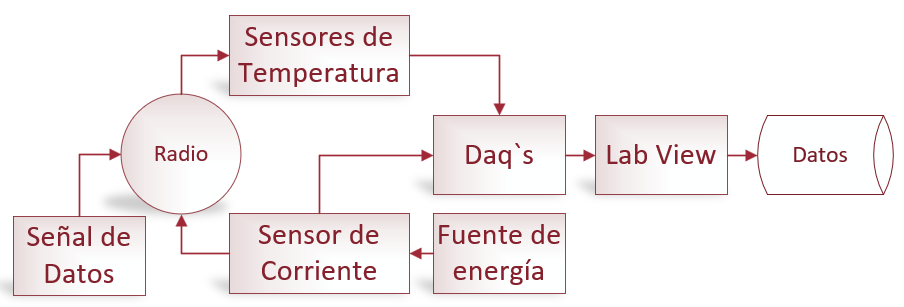
\includegraphics[scale=0.6]{Figuras/adquisicion.png}
\caption{Esquema de adquisición de datos}
Fuente: Elaboración Propia
\label{esquemaadquisicion}
\end{figure}

La hipótesis de experimentación se basa en que para lograr inducir una respuesta térmica en el radio se debe realizar un envió de paquetes de datos que simulen una transmisión, de manera tal que se correlacionen parámetros de transmisión, energía empleada y el aumento de temperatura lo cual no se logra con el baud rate o tasa de baudios la cual es de 1200 o 9600 propias de transmisiones en $VHF$ y $UHF$, está última se utilizará como parámetro fijo junto con la potencia de transmisión, ya que son valores que no tiene una variación durante el momento de la transmisión. Por otra parte se creía hasta este punto que el radio se apagaba durante las transmisiones debido a un circuito de protección térmica que desconectaba el mismo para evitar daños.

\subsection{Paquete de Datos}Esta constituido por líneas de información básica propia de la misión como la fecha, la hora en que se tomó la medición, datos de temperatura, humedad y nivel del humedal que se agrupan en un paquetes de líneas, en donde la cantidad de líneas es ajustable, ya que hasta el momento de las pruebas no se contaba con un tamaño de paquetes definido, sin embargo una línea no representa necesariamente el paquete de datos que envía el radio durante la transmisión, el mismo divide la información en lo que se conoce como tramas compuestas por un total de 276 Bytes máximo distribuidos de la siguiente manera:

\begin{table}[H]
\centering
\caption{Distribución de Bytes en una trama de información }
\label{trama}
\begin{tabular}{lc}
\toprule
\textbf{Sección}     & \textbf{Bytes} \\ \midrule
\textbf{Cabeceras}   & 2              \\
\textbf{Direcciones} & 14             \\
\textbf{Control}     & 1              \\
\textbf{PID}         & 1              \\
\textbf{Datos}       & 256            \\
\textbf{FCS}         & 2              \\ \bottomrule
\end{tabular}
\end{table}

Como se observa en la Tabla \ref{trama}, 18 de los 276 bytes son datos que acompañan a la información que se desea enviar; las cabeceras son un byte de información tanto al inicio como al final que indica cuando inicia un mensaje y cuando termina; las direcciones indican el destino de la información, luego se tiene un byte de control junto con uno de $PID$ o Identificador de paquete y dos bytes de $FCS$ o verificador de secuencia, el cual se encarga de corroborar la integridad de la información.


Es importante hacer la diferencia de que el baud rate no es lo mismo que el data rate o bit rate, es decir, las señales o símbolos por segundo no son iguales a los bits por segundo; la relación entre ellos esta definida por el esquema de modulación, que en este caso es el G3RUH, típico de sistemas en $VHF$ y $UHF$.

\subsection{Tiempo de transmisión} 

Depende directamente de la cantidad de líneas que contenga el paquete de datos; el radio una vez recibe la señal de transmitir abre el canal correspondiente y se mantiene enviando la información seccionada en tramas hasta que termine de enviar el paquete completo y cierre de nuevo el canal. Por otro lado se tiene el tiempo entre tramas que es el delay que puede o no existir entre las tramas o paquetes enviados.

\subsection{Parámetros de experimentación}\label{prueba}

Tomando en cuenta lo expuesto en las secciones anteriores, en la Figura \ref{diagrama_entrada_salida} se expone la propuesta de parámetros que se controlarán entre un experimento y otro, además de los datos que se esperan obtener al final de los experimentos.

\begin{figure}[H]
\centering
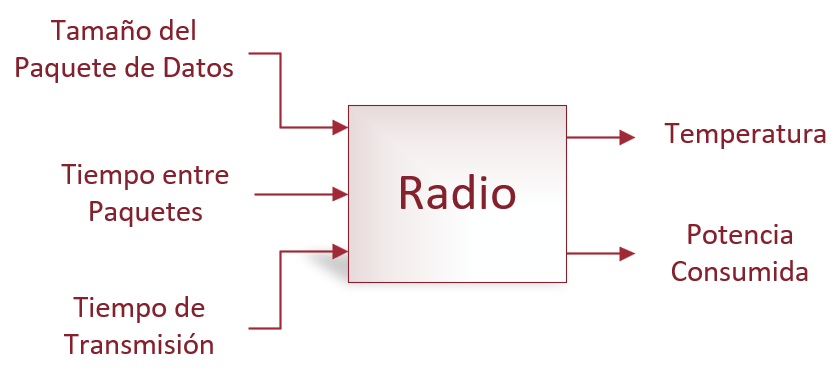
\includegraphics[scale=0.4]{Figuras/entradasalida.png}
\caption{Diagrama de Entradas y Salidas}
Fuente: Elaboración Propia
\label{diagrama_entrada_salida}
\end{figure}

Por otro lado  se dejaron como parámetros fijos en los experimentos:

\begin{table}[H]
\centering
\caption{Parámetros fijos de transmisión}
\label{fijos}
\begin{tabular}{lc}
\toprule
\textbf{Parámetro}           & \textbf{Valor} \\ \midrule
\textbf{Baud Rate (baudios)} & 9600           \\
\textbf{Frecuencia (\si{\mega\hertz})}    & 436            \\
\textbf{\begin{tabular}[c]{@{}l@{}}Potencia de\\ Transmisión (\si{\watt})\end{tabular}} & MID \\
\textbf{Canal}               & UHF            \\ \bottomrule
\end{tabular}
\end{table}

Todas las variables presentadas en la Tabla \ref{fijos} tiene relación de una forma u otra con el comportamiento térmico de radio, sin embargo al encontrarse relacionadas entre sí, un cambio en uno de estos parámetros podría implicar una variación en los demás, debido a que el baud rate está definido mediante un estándar que establece la frecuencia de la honda portadora de envió; a su vez las frecuencias están relacionadas con el canal, el cual implica un MOSFET en específico ya sea el de $VHF$ o el de $UHF$, es decir cada uno de los dos módulos de potencia (MOSFET) puede enviar o recibir datos dentro de un margen de frecuencias específico que no es el mismo entre ellos. Los encargados de realizar el enlace, determinaron que la potencia de transmisión  seleccionada era la suficiente para lograr transmitir los datos y para efectos de experimento se espera tener la condición que provoque mayor esfuerzo para el radio, lo cual en este caso sería en potencia media ya que de antemano se conocía que el radio se apagaba si se utilizaba en la máxima potencia; se retomará este tema cuando se realice el análisis de resultados. 

\section{Resultados obtenidos}

\subsection{Resultados Preliminares}

Previo a los experimentos formales, se realizaron pruebas preliminares, para determinar el comportamiento del radio, con el fin de establecer los valores de los parámetros en los experimentos de manera tal que se pudiera obtener la mayor cantidad de información posible, para lo cual se recurrió al micrófono del mismo, que de ahora en adelante se le conocerá como PTT (``Push to talk''); el cual permite simular una transmisión ya que tiene el mismo efecto sobre el módulo de potencia.

\begin{figure}[H]
\centering
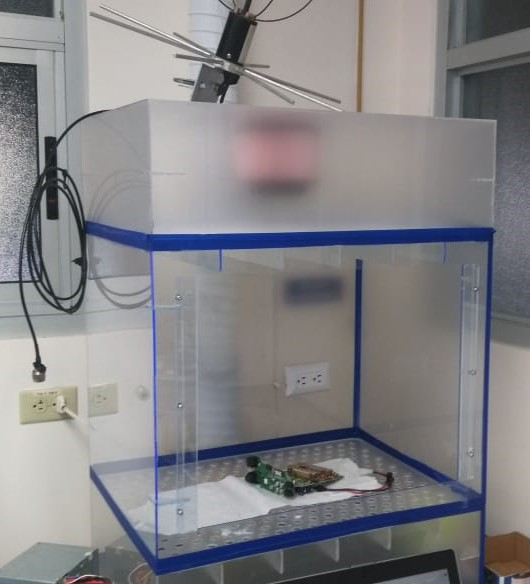
\includegraphics[scale=0.6]{Figuras/campana.jpeg}
\caption{Sitio de pruebas}
Fuente: Elaboración Propia
\label{campana}
\end{figure}


En la Figura \ref{campana} se muestran el lugar donde se colocó el radio, no se muestra todos los dispositivos utilizados para la realización de las pruebas. El recinto originalmente es utilizado para realizar montajes de dispositivos electrónicos bajo ambientes controlados (libre de polvo y partículas); la idea de realizar las pruebas en este sitio era la de eliminar en la medida de lo posible los efectos convectivos que son el resultado de corrientes de aire presentes en el laboratorio.

Para la prueba preliminar se utilizó el PTT en accionamientos que duraban 5 segundos aproximadamente y con un tiempo entre cada accionamiento de 5 segundos también, con intención de corroborar la hipótesis de que estos parámetros tienen un impacto en el comportamiento térmico significativo en el radio; la aproximación del tiempo se debe a que utilizar el PTT implica un proceso manual. Los resultados se muestran a continuación.

\begin{figure}[H]
\centering
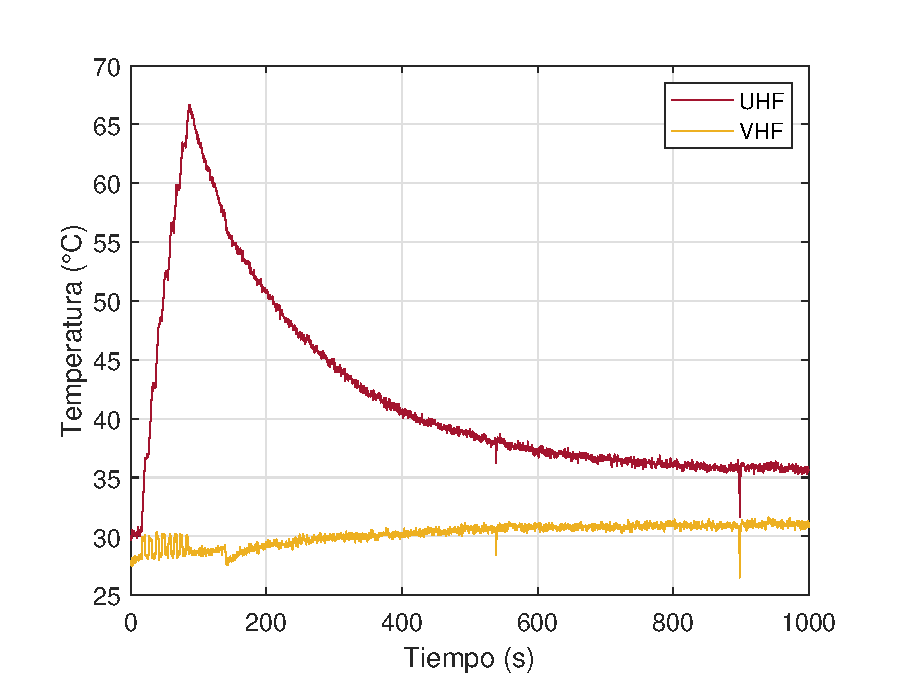
\includegraphics[scale=0.80]{Figuras/preliminar1.eps}
\caption{Gráfico Temperatura vs tiempo para los dos módulos de potencia}
Fuente: Elaboración Propia
\label{preliminar1}
\end{figure}

De la prueba realizada y de los datos mostrados en la Figura \ref{preliminar1} se obtienen la siguientes conclusiones y anotaciones:

\begin{itemize}
    \item Se confirma que durante la transmisión solo uno de los módulos de potencia permanece activo, el segundo presenta un leve incremento, mas no representativo y el cual podría está ligado a otras causas por lo que para efectos de las siguientes pruebas todos los datos mencionados hacen referencia al módulo de potencia de $UHF$.
    \item El incremento de temperatura presenta un comportamiento con una pendiente  elevada, lo cual confirma la necesidad térmica planteada y a su vez, que los parámetros de experimentación seleccionados, son representativos y al controlarlos se pueden obtener diferentes comportamientos térmicos.
    \item El rápido incremento en la temperatura pone de manifiesto la advertencia de no exceder los valores de temperatura de operación de los módulos de potencia, por el daño y degradación que los mismos podrían sufrir,esto implica que el tiempo de transmisión se vuelve relevante tanto para los experimentos como para la operación dentro de la estación remota. 
    \item El tiempo aproximado de transmisión fue de 2 minutos, sin embargo bajo condiciones de convección natural disminuidas el radio tarda aproximadamente 15 minutos en alcanzar una temperatura estable, pero aún así por encima de la inicial.
    
\end{itemize}

\subsection{Experimentos planteados}

Se plantearon 4 experimentos formales de los cuales se obtuvo información para realizar el modelo matemático del radio y poder realizar comparaciones.

\begin{table}[H]
\centering
\caption{Parámetros de entrada en los experimentos}
\label{parametros_experimento}
\begin{tabular}{lcccc}
\toprule
\multicolumn{1}{c}{\multirow{2}{*}{\textbf{Parámetro}}} & \multicolumn{4}{c}{\textbf{Experimento}}                                                              \\ \cline{2-5} 
\multicolumn{1}{c}{}        & \textbf{1} & \textbf{2} & \textbf{3} & \textbf{4} \\ \midrule
Tamaño de paquete (Bytes)                               & \multicolumn{1}{l}{4000} & \multicolumn{1}{l}{4000} & \multicolumn{1}{l}{42} & \multicolumn{1}{l}{42} \\ 
Tiempo de transmisión (\si{\min}) & 4:57       & 4:51       & 1          & 1          \\
Tiempo entre paquetes (\si{\second})     & 8         & 10          & 1          & 5          \\
Voltaje Real (\si{\volt}) & \multicolumn{4}{c}{12.12}\\
Temperatura ambiente (\si{\celsius}) & \multicolumn{4}{c}{24}\\ 
\bottomrule
\end{tabular}
\end{table}

En cuanto al tamaño del paquete los primeros dos experimentos se realizaron con un archivo de datos de prueba que se utilizaba para comprobar la programación de la transmisión para el caso de los experimentos 3 y 4 se ajustó el tamaño del paquete al de una línea de información. Los tiempos de transmisión se determinaron según las predicciones realizadas por el laboratorio de los tiempos de pasadas óptimas, es decir, el tiempo durante el cual el satélite pasa dentro de un rango de área que permite el enlace satelital con el radio de la estación remota, mientras el mismo orbita sobre la tierra. Los estudios indicaron que para la órbita del satélite y las condiciones geográficas de Palo Verde las pasadas promedio tienen una duración aproximada de 5 minutos, mientras que el tiempo mínimo de una pasada ronda el minuto. Por último, el tiempo entre paquetes se determinó basado en la experiencia de las pruebas preliminares.

\subsection{Datos obtenidos}

A continuación se muestran los resultados obtenidos de los cuatro experimentos:

\textbf{Experimento 1:}

\begin{figure}[H]
\centering
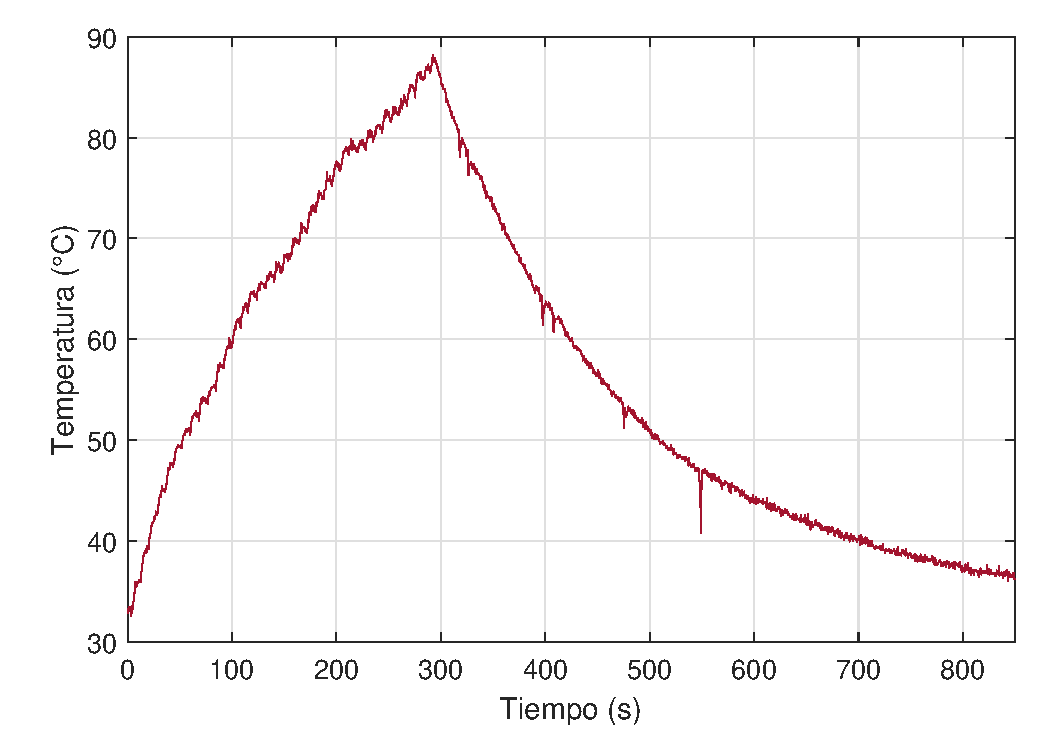
\includegraphics[scale=0.65]{Figuras/Exp2_T.eps}
\caption{Gráfico Temperatura vs tiempo para el Experimento 1}
Fuente: Elaboración Propia
\label{exp1_T}
\end{figure}

\begin{figure}[H]
\centering
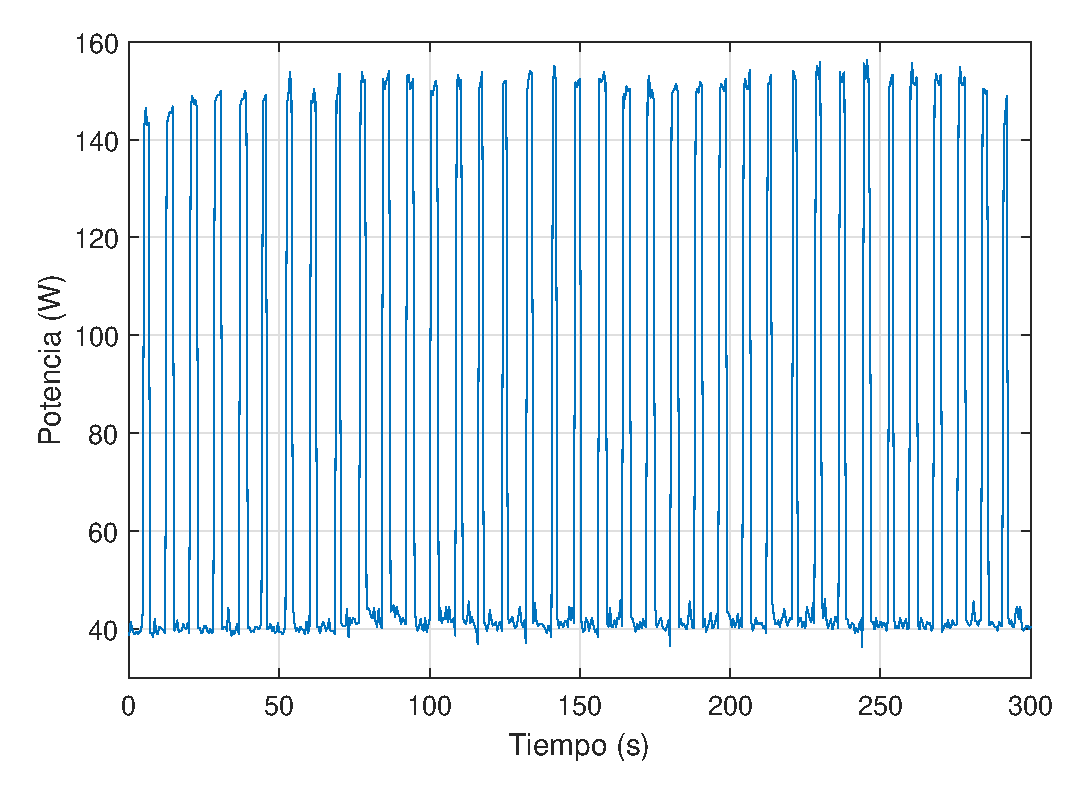
\includegraphics[scale=0.65]{Figuras/Exp2_P.eps}
\caption{Gráfico Potencia vs tiempo para el Experimento 1}
Fuente: Elaboración Propia
\label{exp1_P}
\end{figure}

\textbf{Experimento 2:}

\begin{figure}[H]
\centering
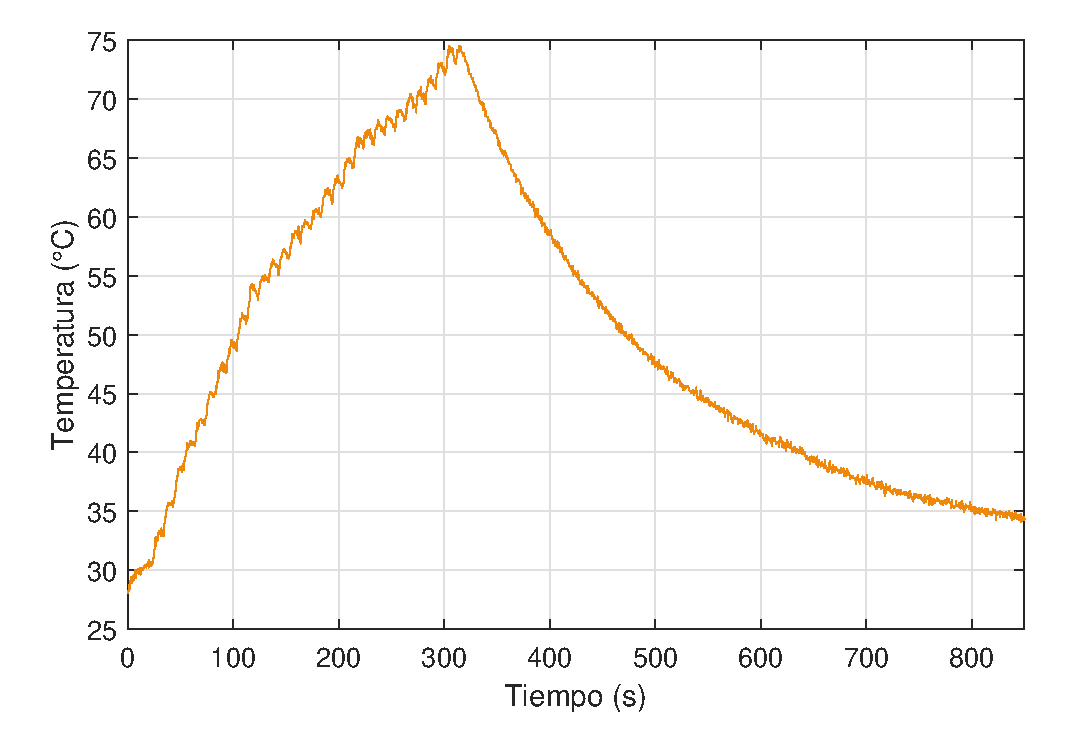
\includegraphics[scale=0.64]{Figuras/Exp1_T.eps}
\caption{Gráfico Temperatura vs tiempo para el Experimento 2}
Fuente: Elaboración Propia
\label{exp2_T}
\end{figure}

\begin{figure}[H]
\centering
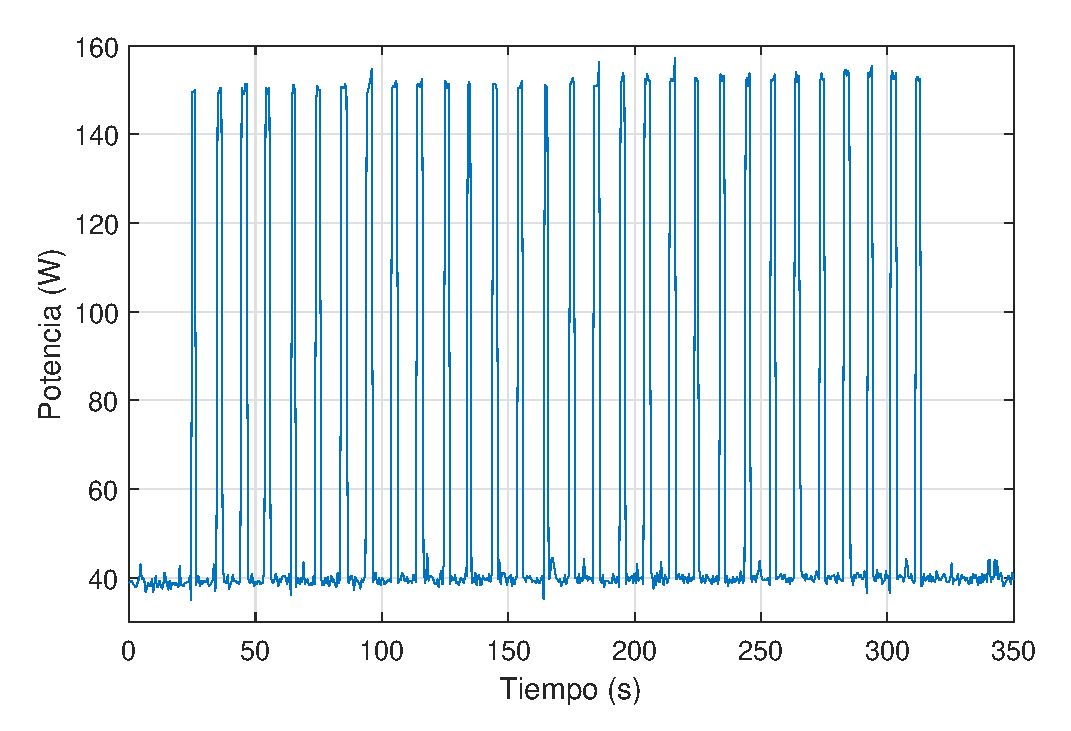
\includegraphics[scale=0.66]{Figuras/Exp1_P.eps}
\caption{Gráfico Potencia vs tiempo para el Experimento 2}
Fuente: Elaboración Propia
\label{exp2_P}
\end{figure}
%Tuve un error en el orden los experimentos al guardar los graficos por eso el nombre de las figuras esta invertido
\textbf{Experimento 3:}

\begin{figure}[H]
\centering
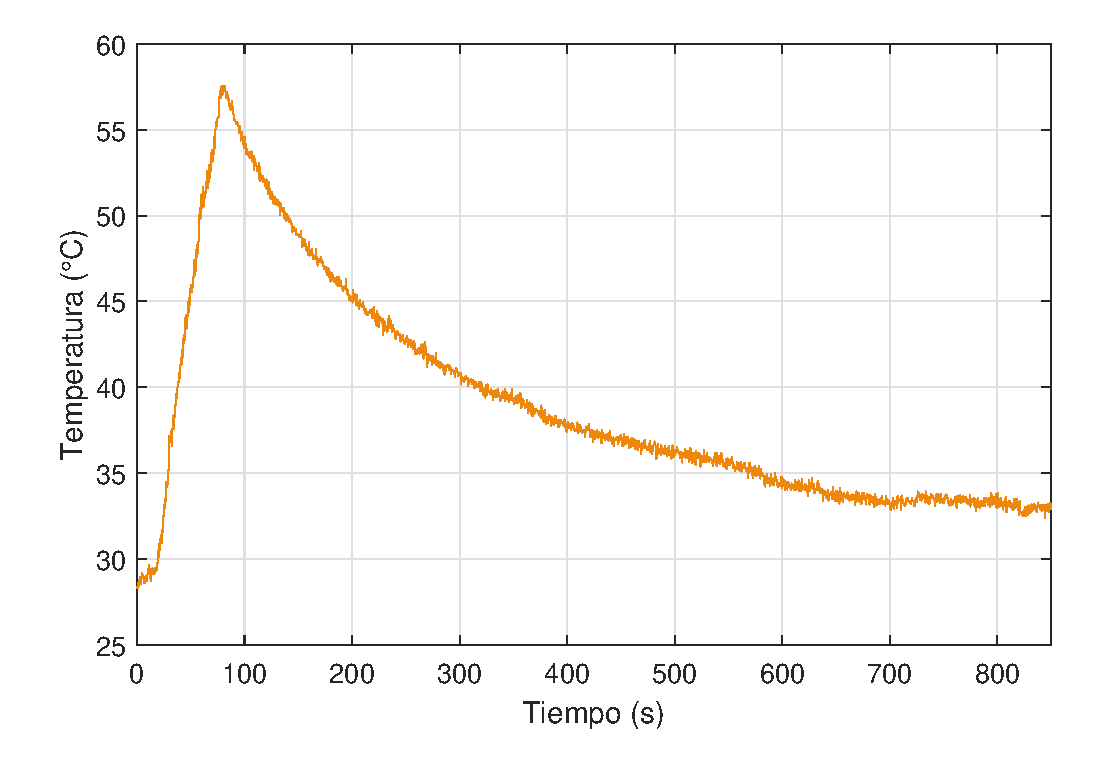
\includegraphics[scale=0.65]{Figuras/Exp4_T.eps}
\caption{Gráfico Temperatura vs tiempo para el Experimento 3}
Fuente: Elaboración Propia
\label{exp4_T}
\end{figure}

\begin{figure}[H]
\centering
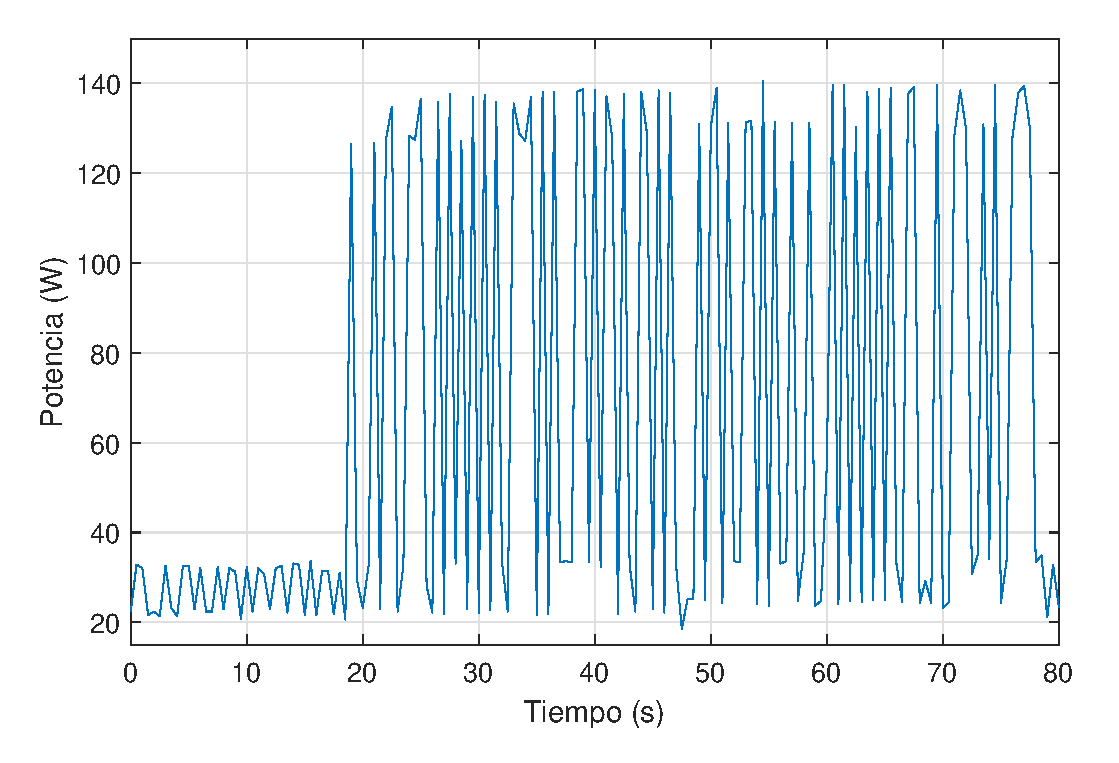
\includegraphics[scale=0.66]{Figuras/Exp4_P.eps}
\caption{Gráfico Potencia vs tiempo para el Experimento 3}
Fuente: Elaboración Propia
\label{exp4_P}
\end{figure}

\textbf{Experimento 4:}

\begin{figure}[H]
\centering
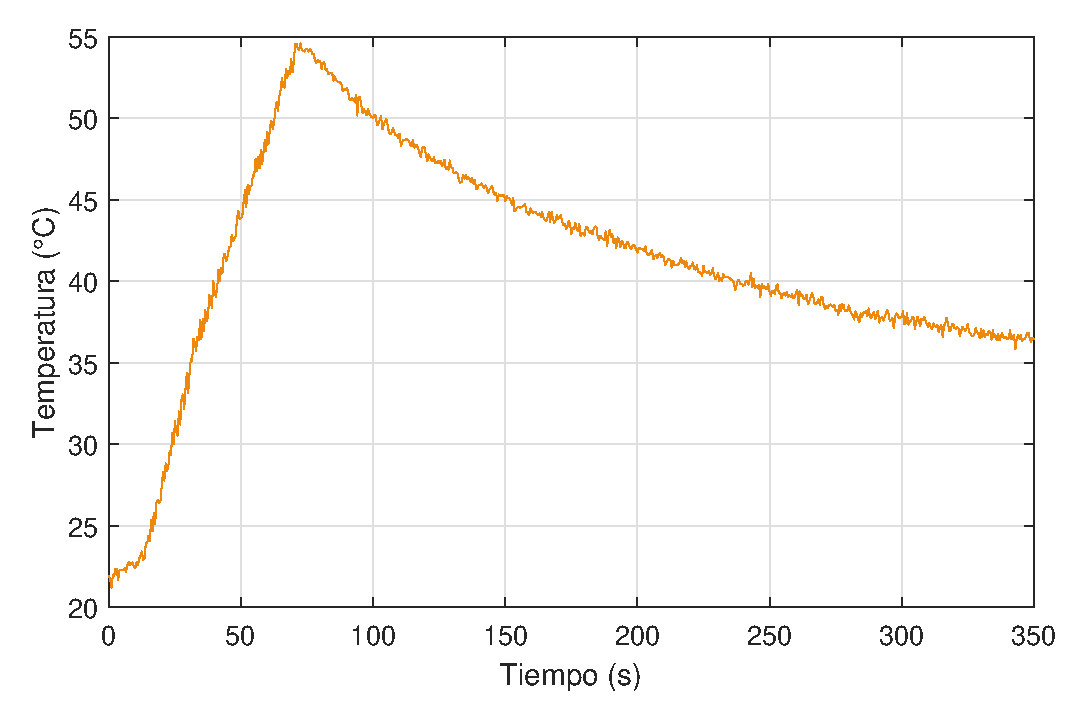
\includegraphics[scale=0.65]{Figuras/Exp3_T.eps}
\caption{Gráfico Temperatura vs tiempo para el Experimento 4}
Fuente: Elaboración Propia
\label{exp3_T}
\end{figure}

\begin{figure}[H]
\centering
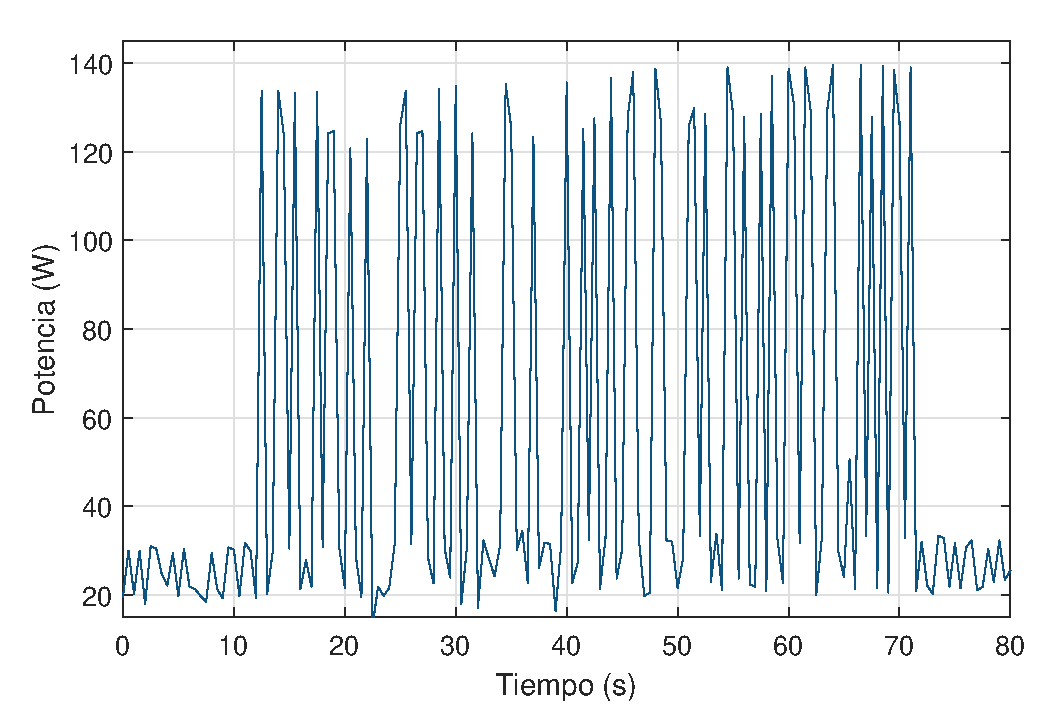
\includegraphics[scale=0.65]{Figuras/Exp3_P.eps}
\caption{Gráfico Potencia vs tiempo para el Experimento 4}
Fuente: Elaboración Propia
\label{exp3_P}
\end{figure}

\subsection{Análisis de Resultados:}

De los datos mostrados anteriormente se obtienen las siguientes conclusiones:

\begin{enumerate}
    \item Se comprueba la hipótesis de la relación existente entre el tamaño del paquete, el tiempo entre paquetes y la temperatura alcanzada por el módulo de potencia.
    
    \item Gracias a los experimentos se determinó que la causa del fallo en las transmisiones que se atribuían al radio, se debía a un daño y a la mala selección en la fuente de poder, ya que las corrientes las cuales no se muestran en este caso, excedían la capacidad de la fuente utilizada, y no se debía al circuito de protección como se pensaba, el cual se determinó en el manual que su función no es apagar el radio, sino más bien, si el mismo se encontraba en máxima potencia, el circuito, luego de cierta temperatura (la cual nunca se especifíca en el manual), bajará automáticamente el radio a la potencia mínima. Esto descarta la hipótesis que se tenía al inicio de este proyecto la cual supone que el calentamiento provocaba fallos en el radio.
    
    \item En ninguno de los cuatro casos se supera el límite de temperatura de 100\degree C establecido en el datasheet del módulo de potencia, el Experimento 1 el más cercano a este punto. Sin embargo, existen dos aspectos a considerar; el primero es que el Experimento 1 establece parámetros restrictivos de transmisión para el radio, es decir utilizar dichos parámetros u otros que representen un mayor esfuerzo térmico para el radio, podrían implicar degradación térmica de los componentes del módulo de potencia; por otra parte se debe aclarar que el límite de 100\degree C es especifico del módulo, mientras que el rango de operación máximo del radio de 60\degree C hace referencia a las condiciones generales y ambientales operativas del radio y dichos límites se deben considerar dentro los respectivos contextos.
    
    \item En la Figura \ref{comparacion} se muestra el gráfico comparativo de las temperaturas obtenidas en los cuatro experimentos, en donde se observa como la pendiente o bien el comportamiento de la curva varia con el tiempo entre paquetes y con el tamaño del paquete. Los cuatro experimentos plantean condiciones límites de parámetros de transmisión, ya que como se observa se debe tener un equilibrio entre el tamaño del paquete y el tiempo entre tramas o paquetes para lograr un perfil térmico de manera tal, que se pueda enviar la mayor cantidad de información dentro de los tiempos promedio de transmisión.
    
     \item La hipótesis inicial plantea que dentro de los valores mostrados en la Tabla \ref{parametros_experimento} se establecieron los tiempos entre paquetes; sin embargo al observar detenidamente los valores de potencia obtenidos en los experimentos se observa que el tiempo ingresado como parámetro es en realidad el tiempo de ciclo de trabajo que comprende tanto el tiempo de envió como el tiempo de delay entre paquetes.
    \item Del mismo análisis de la señal de potencia, se observa que existen irregularidades en los tiempos de transmisión para los experimentos 3 y 4, ya que se debe recordar, que aún cuando el paquete sea una línea de información, esto no quiere decir que se trate de una trama, con lo que se comprueba que internamente el radio segmenta la información de manera que para estos casos en específico se dificulta la identificación de un patrón; sin embargo dichos experimentos siguen representando el mejor perfil de transmisión para el radio desde una perspectiva térmica.
 
\end{enumerate}

\begin{figure}[H]
\centering
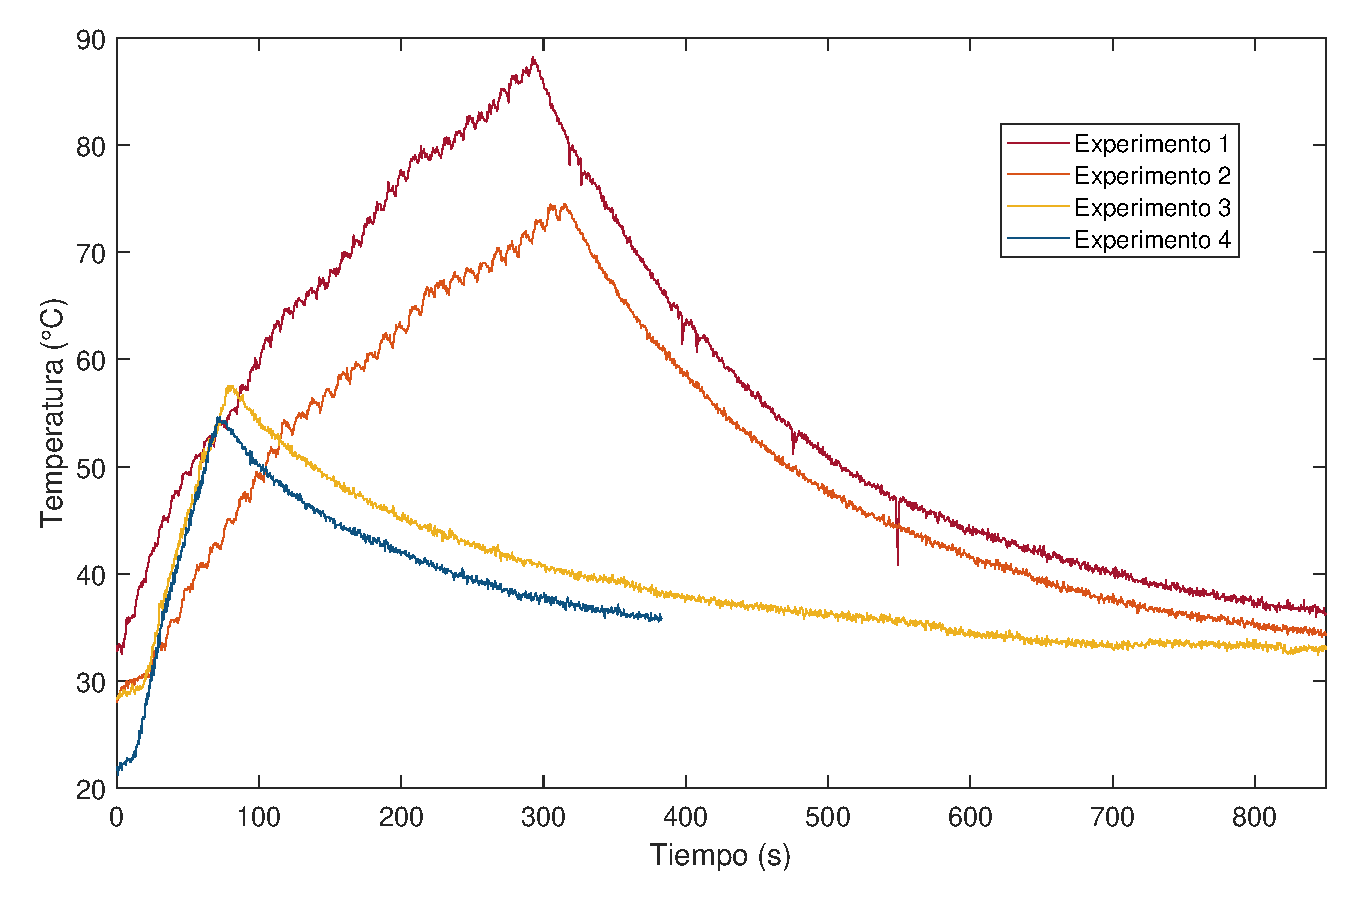
\includegraphics[width=\linewidth]{Figuras/comparacion.eps}
\caption{Gráfico Potencia vs tiempo para el Experimento 4}
Fuente: Elaboración Propia
\label{comparacion}
\end{figure}

Por otra parte en los Anexos \ref{anexo12},\ref{anexo13},\ref{anexo14},\ref{anexo15} se presentan parte del montaje utilizado para la realización de los experimentos.

\newpage
\section{Modelo Térmico del Radio}

Después de realizar el análisis respectivo de los datos obtenidos de los experimentos, se requería correlacionar los datos de potencia con el comportamiento térmico del radio; por lo que se recurrió a las herramientas de Matlab y Simulink para la implementación de una función de transferencia que relacione estas dos variables y en conjunto con la simulación de parámetros térmicos, se pueda obtener el perfil de temperatura obtenido en los experimentos; para lo cual se plantea el esquema de modelado de la Figura \ref{esquema_modelo_radio}. 

\begin{figure}[H]
\centering
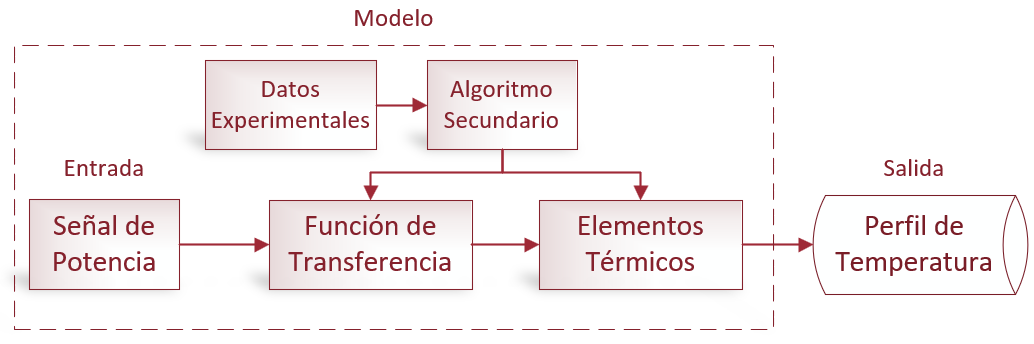
\includegraphics[scale=0.52]{Figuras/esquema_modelo_radio.png}
\caption{Esquema de modelo para el radio transmisor}
Fuente: Elaboración Propia
\label{esquema_modelo_radio}
\end{figure}

 A continuación se explica brevemente en que consiste cada bloque del esquema de modelado.
 
 \begin{itemize}
     \item \textbf{Datos Experimentales:} Son la base del modelo, ya que con esta información se obtendrán los datos del flujo de calor generado por el radio y establece a través de herramientas matemáticas la relación potencia-temperatura. Se seleccionaron los datos del experimento 2 para la elaboración del modelo debido a la homogeneidad en los datos de potencia; además los datos del experimento 1 representan un caso de parámetros límites de transmisión para el radio, por lo que para efectos del diseño son datos no deseables.
     \item \textbf{Algoritmo Secundario:} Comprende toda la parte de programación y cálculos que dan soporte a la función de transferencia y a los elementos de programación que simulan el comportamiento térmico; en este punto es de donde se determina la función de transferencia, para este caso se utiliza la función predeterminada de matlab \textit{tfest(data, np, nz)}, donde $np$ es la cantidad de polos y $nz$ es la cantidad de ceros.
     \item \textbf{Función de transferencia:} Hace referencia a su aplicación; se utilizó un número de polos de 5 y por ende 4 ceros. Su trabajo  es recibir los pulsos o señal de potencia eléctrica y convertirlos en un nivel de flujo de calor en un comportamiento determinado por la función misma.
     \item \textbf{Señal de Potencia:} Es la parte encargada de simular el comportamiento real de los pulsos de potencia eléctrica observados durante los experimentos y asociarlos a parámetros como tiempo de transmisión, tiempo entre paquetes, valor de potencia tanto en trasmisión como en reposo,entre otros; de manera tal que por medio de este bloque se pueda estimar el comportamiento térmico del radio al considerar diferentes parámetros de envió de datos. Este bloque a su vez representa una entrada virtual del modelo.
     \item \textbf{Elementos Térmicos:} Corresponde específicamente a la forma en que el software interpreta los diferentes mecanismos de transferencia de calor y los interconecta y relaciona matemáticamente con los demás elementos que conforman el modelo. 
     \item \textbf{Perfil de temperaturas:} Representa la salida del modelo, el cual luego de procesar la entrada, arroja como resultado el perfil de temperaturas asociado a los parámetros de potencia introducidos.
 \end{itemize}
 
En los Anexos \ref{anexo7} y \ref{anexo8} se muestra el algoritmo que se utilizó para simular el comportamiento de radio. En la Figura \ref{fit} se muestran los resultados superpuestos entre los datos experimentales y la curva de mejor ajuste obtenida mediante la función de transferencia, la cual tiene una aproximación de los datos reales en un \SI{96,18}{\percent} cuando se comparan los flujos de calor obtenidos del experimento 2.

\begin{figure}[H]
\centering
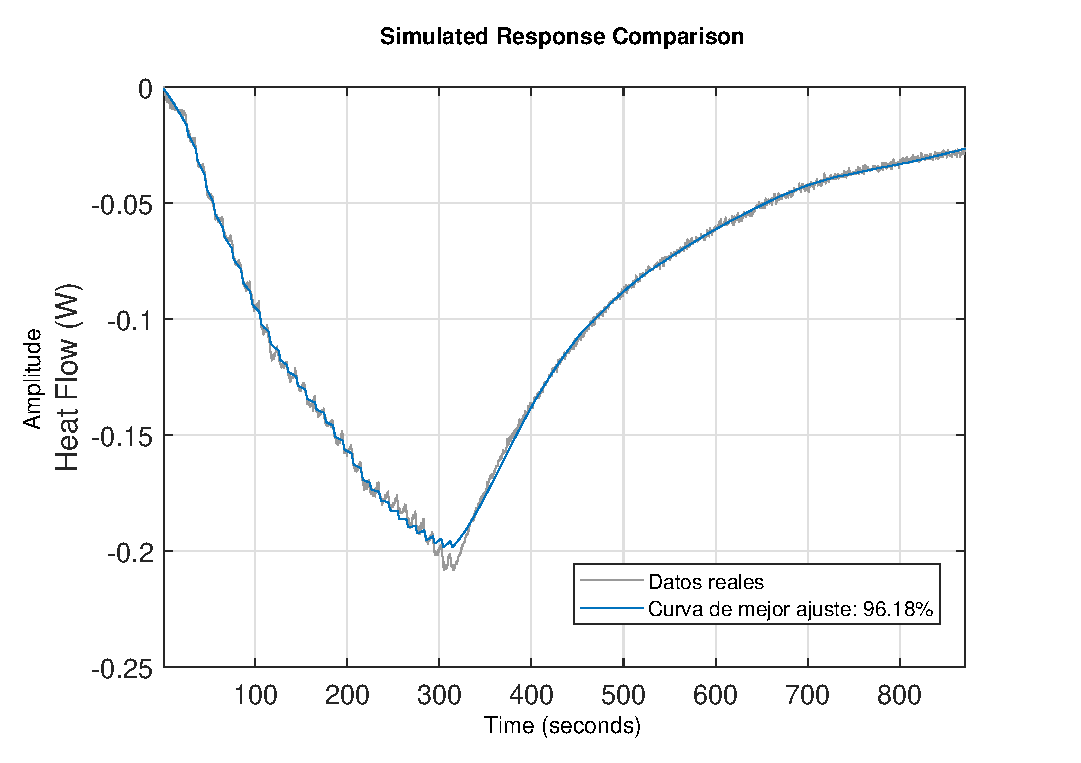
\includegraphics[scale=0.70]{Figuras/Fit.eps}
\caption{Gráfico comparativo entre los datos experimentales y la curva de mejor ajuste}
Fuente: Elaboración Propia
\label{fit}
\end{figure}

Para realizar los cálculos del flujo de calor se partió de la Ecuación \ref{Newton}, modelando la situación del radio en los experimentos como convección natural en entre la placa del módulo y el aire circundante, para lo cual se utilizaron los datos mostrados en la Tabla \ref{datosflujo}

\begin{table}[H]
\centering
\caption{Datos utilizados en la determinación del flujo de calor}
\label{datosflujo}
\begin{tabular}{lc}
\toprule
$h$ (\si{\watt/\meter\squared\celsius}) & 5 \\ % Mejor \SI{}{\watt/\meter\squared\degree} 
Área modulo (\si{\meter\squared}) & $8,964\times 10^{-4}$ \\ \bottomrule
\end{tabular}
\end{table}

La determinación del coeficiente de convección se establece a partir de la información en la literatura para convección natural \cite{redfrio}; más adelante para el modelo completo de la estación y considerando la posición del módulo de potencia, se realizará un cálculo más preciso de este coeficiente. La razón para determinar la tasa de transferencia de calor al considerar la convección natural radica en no entrar en complejidades técnicas y matemáticas al modelar el MOSFET de potencia desde su capas constructivas, máxime que el datasheet del módulo no contaba con la información suficiente para realizar dicha tarea, y si bien es cierto el módulo es el principal objeto de estudios de este proyecto, las acciones que se pueden realizar sobre el mismo no son internas, no pueden y no deben afectar de ninguna manera aspectos constructivos del módulo; por lo que para efectos de este proyecto es de interés la temperatura superficial que el mismo puede llegar a tener.

\begin{figure}[H]
\centering
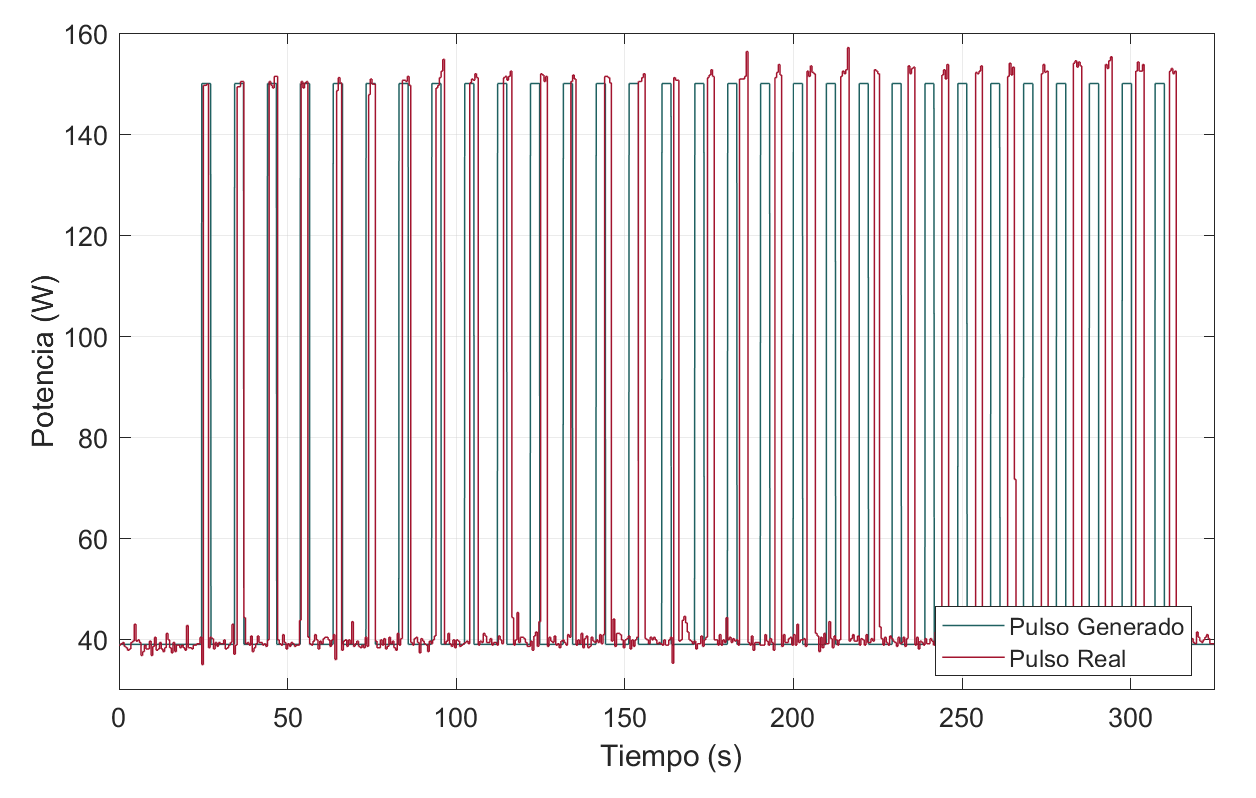
\includegraphics[scale=0.63]{Figuras/Resultado_P.eps}
\caption{Gráfico Potencia vs Tiempo para los resultados del modelado}
Fuente: Elaboración Propia
\label{resultado_P}
\end{figure}

\begin{figure}[H]
\centering
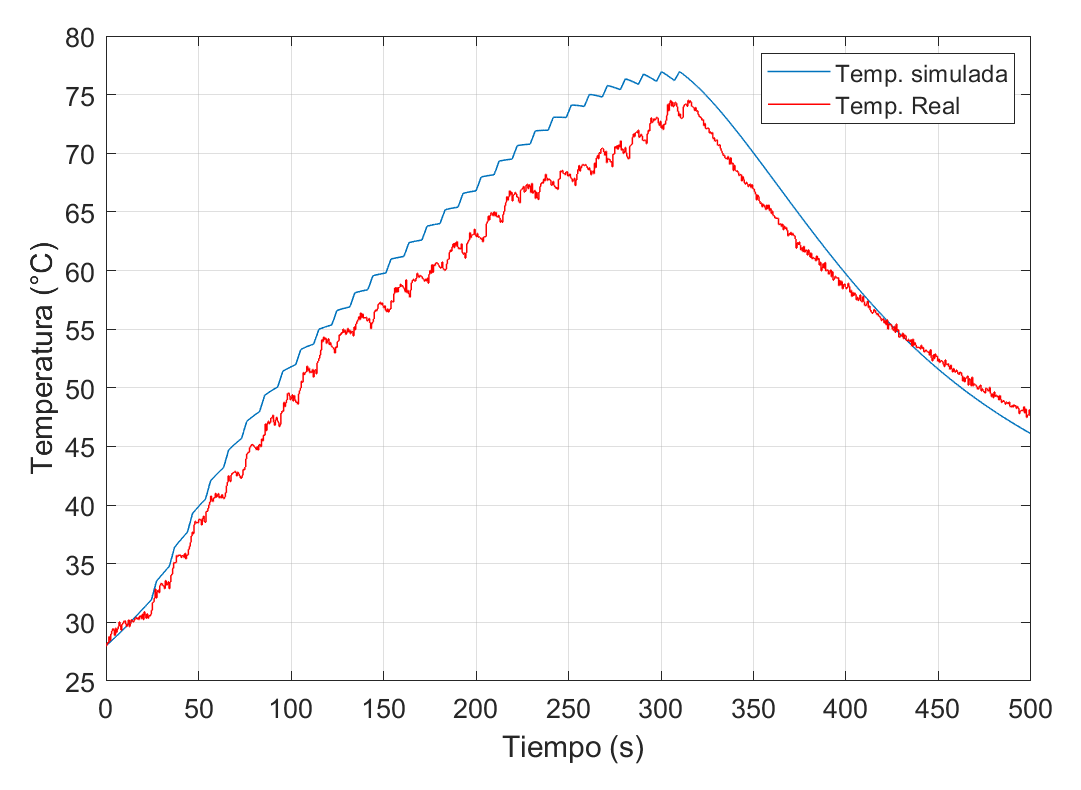
\includegraphics[scale=0.66]{Figuras/Resultado_T.eps}
\caption{Gráfico Temperatura vs Tiempo para los resultados del modelado}
Fuente: Elaboración Propia
\label{resultado_T}
\end{figure}

\begin{figure}[H]
\centering
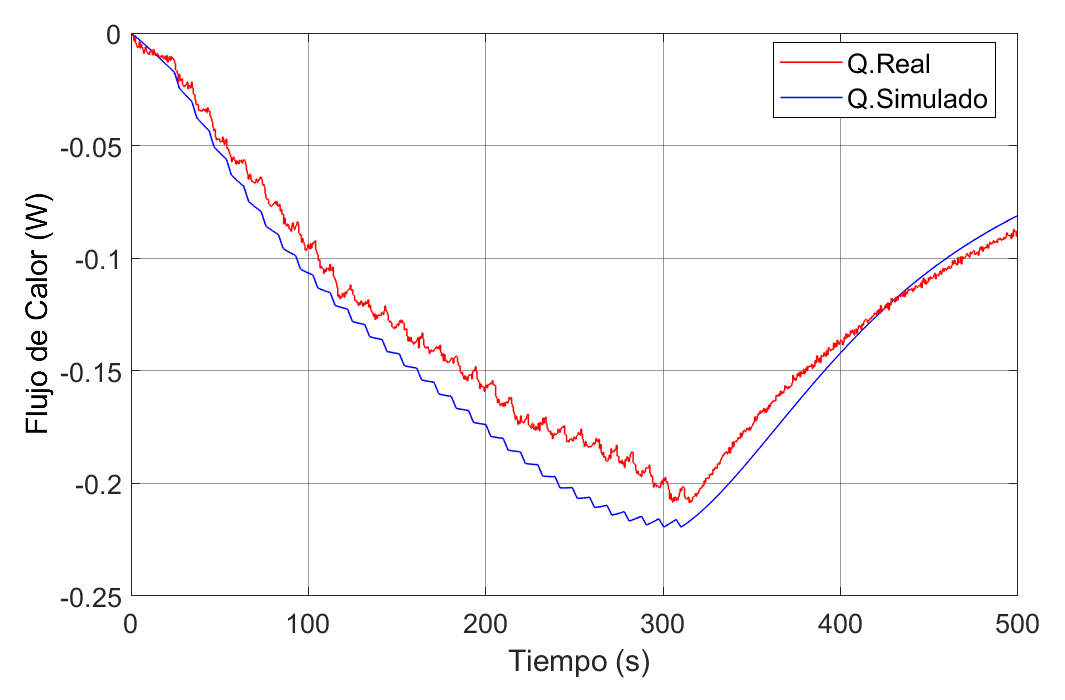
\includegraphics[scale=0.75]{Figuras/Resultado_Q.eps}
\caption{Gráfico Flujo de Calor vs Tiempo para los resultados del modelado}
Fuente: Elaboración Propia
\label{resultado_Q}
\end{figure}

\subsection{Observaciones del Modelo}

De los resultando antes mostrados se logran extraer las siguientes observaciones.

\begin{enumerate}
    \item En la Figura \ref{resultado_P} se hace evidente la irregularidad en los pulsos de potencias emitidos por el radio; ya que, si bien es cierto los primeros pulsos coinciden a la perfección con los simulados y los obtenidos experimentalmente, al transcurrir los segundos empieza a marcase un desfase, seguido de un ligero incremento de la potencia. Esto demuestra que la forma en que el radio transmite la información no es de manera homogénea, ya que básicamente el pulso simulado es una onda cuadrada de parámetros específicos y constantes.
    \item En la Figura \ref{resultado_T} se observa como a pesar de lo expuesto en el punto anterior, el modelo realiza una buena proyección del comportamiento térmico del radio, además de captar de manera óptima el comportamiento de la curva tanto para las temperaturas como para el flujo de calor (Figura \ref{resultado_Q}).
    \item Las principales discrepancias entre los datos reales y los simulados en las temperaturas y en el flujo de calor, se observa que ocurren justamente en el momento en que se dan las diferencias de potencia entre el pulso generado y el pulso medido.
    \item La determinación del coeficiente de convección para este caso fue acertada para las condiciones en las que se realizaron los experimentos que determinaron el modelo.
\end{enumerate}

\section{Validación del Modelo }

Por ser un apartado fundamental del proyecto, el cual por si solo tiene funcionalidad descriptiva, se realizó una validación del modelo construido para el radio transmisor; para lo cual se introdujeron los parámetros de transmisión obtenidos en los experimentos 1 y 3, es decir, se sometió el modelo a la prueba de simular la salida obtenida de los datos experimentales, haciendo uso de la herramienta implementada y se obtuvieron los resultados que se muestran mas adelante, los cuales se subdividen en dos validaciones.

Para ambos casos se utilizaron los mismos datos de la Tabla \ref{datosflujo}, variando los parámetros de transmisión aproximados acorde con los datos usados en los experimentos .Vale la pena anticipar que al igual que en el caso de los resultados del modelo, las aproximaciones de las curvas de calor y de temperatura están acorde con la aproximación de los pulsos de potencia, lo cual se dificultaba principalmente en la primera validación donde se observa que se tiene una situación donde dichos pulsos presentan irregularidades a lo largo de la transmisión; a pesar de ello el modelo nuevamente muestra que puede realizar una buena aproximación del comportamiento térmico del radio, por lo cual es apto para ser implementado en diferentes procesos y etapas del diseño, no solo de este proyecto, sino también de la misión.

\subsection{Primera Validación}

\begin{figure}[H]
\centering
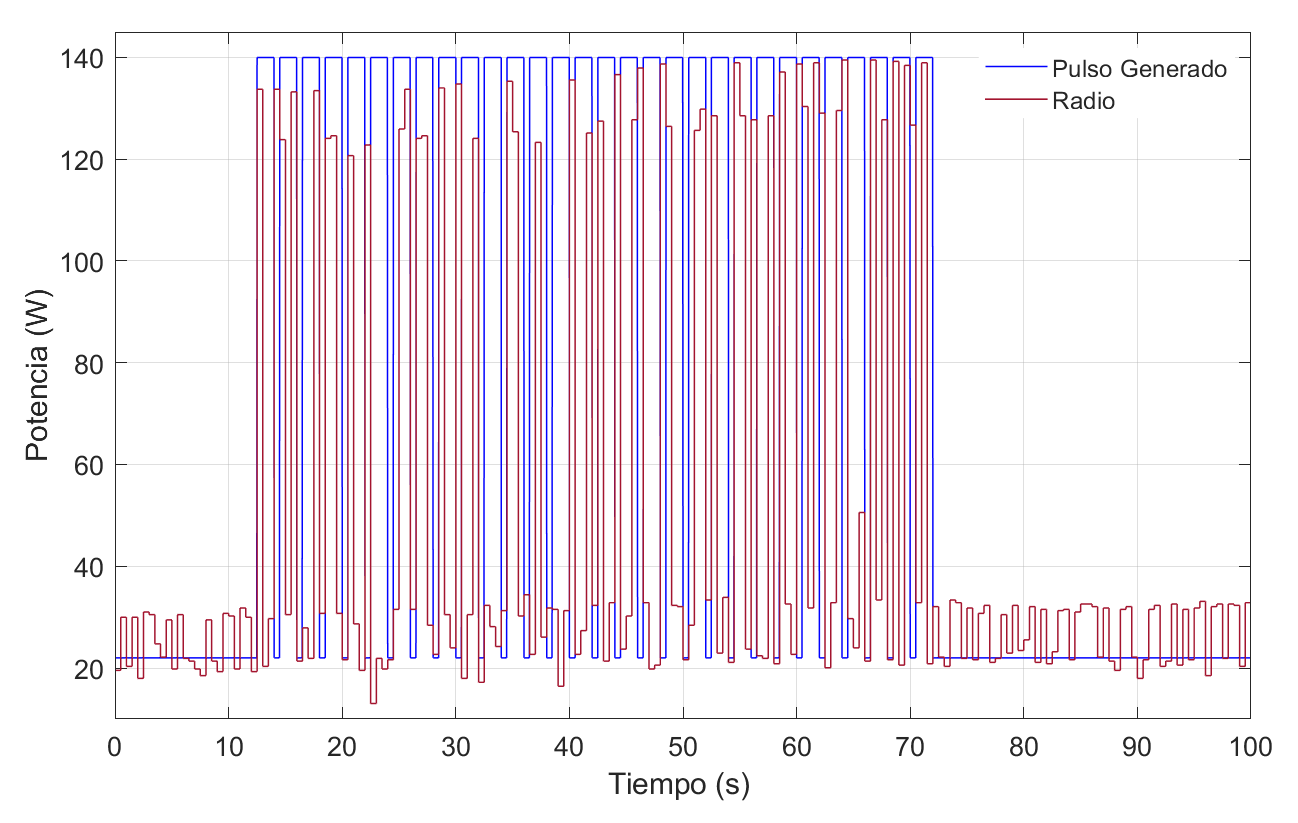
\includegraphics[scale=0.67]{Figuras/Validacion_1_P.eps}
\caption{Gráfico Potencias vs Tiempo de la primera validación}
Fuente: Elaboración Propia
\label{validacion_1_P}
\end{figure}

\begin{figure}[H]
\centering
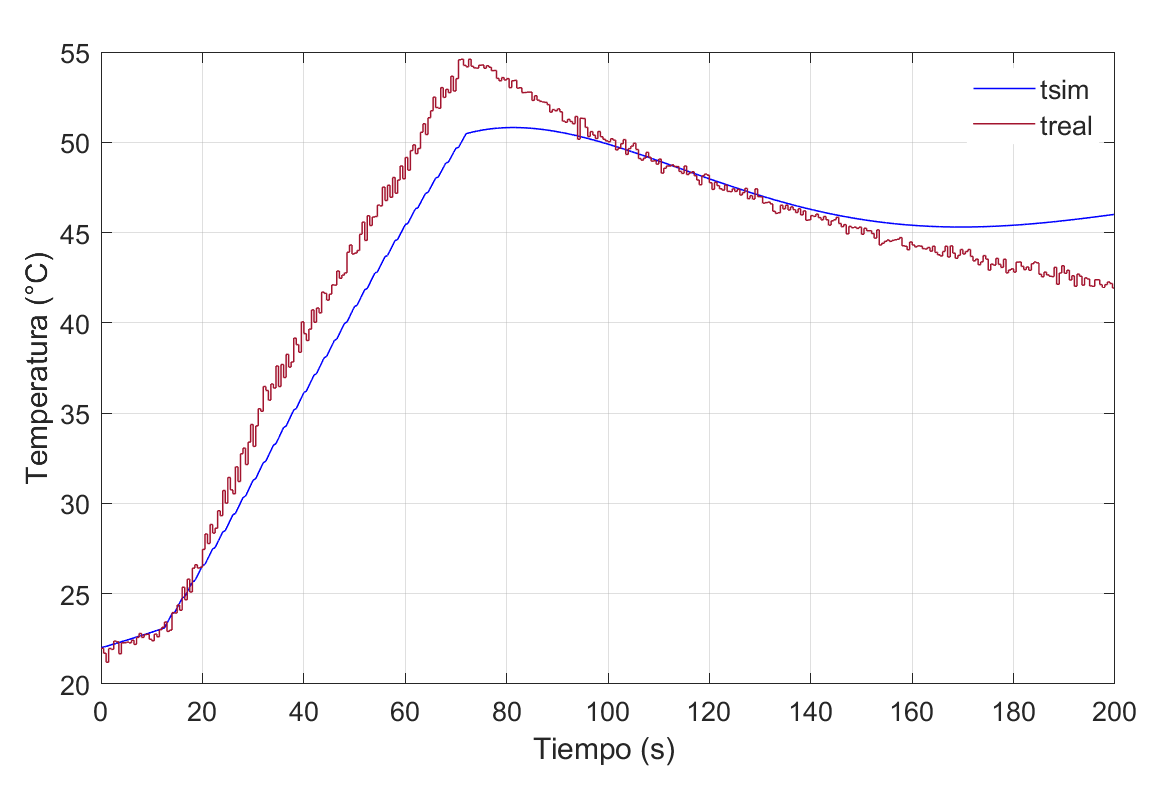
\includegraphics[scale=0.66]{Figuras/Validacion_1_T.eps}
\caption{Gráfico Temperaturas vs Tiempo de la primera validación}
Fuente: Elaboración Propia
\label{validacion_1_T}
\end{figure}

\begin{figure}[H]
\centering
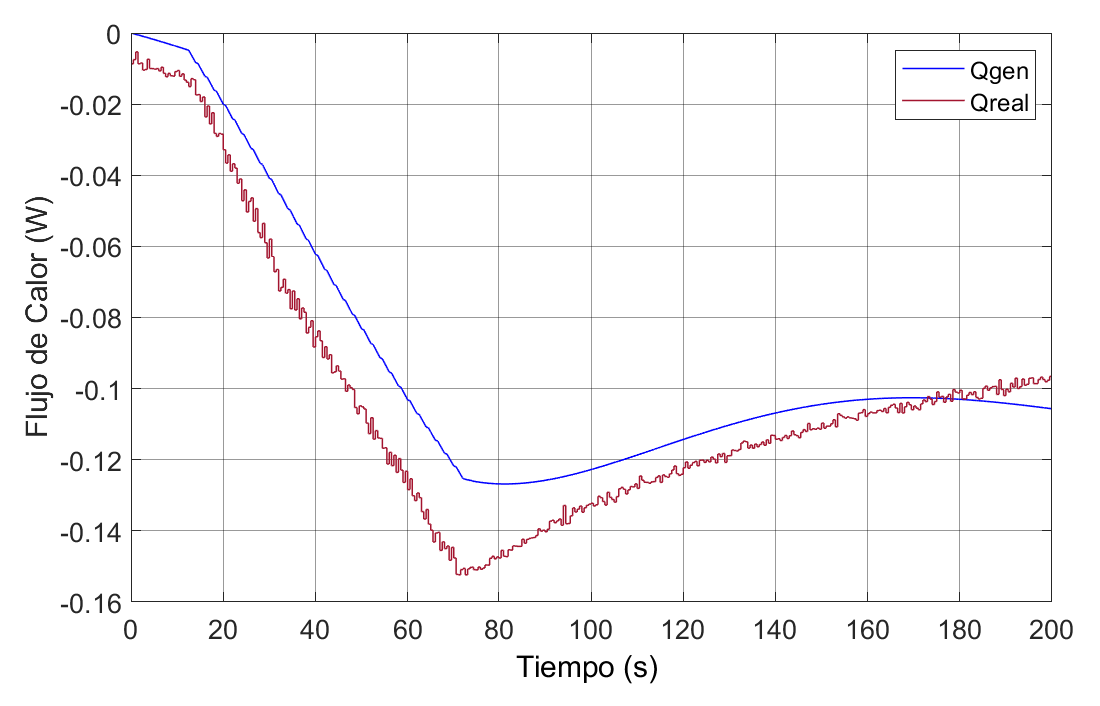
\includegraphics[scale=0.68]{Figuras/Validacion_1_Q.eps}
\caption{Gráfico Flujos de Calor vs Tiempo de la primera validación}
Fuente: Elaboración Propia
\label{validacion_1_Q}
\end{figure}

\subsection{Segunda validación}

\begin{figure}[H]
\centering
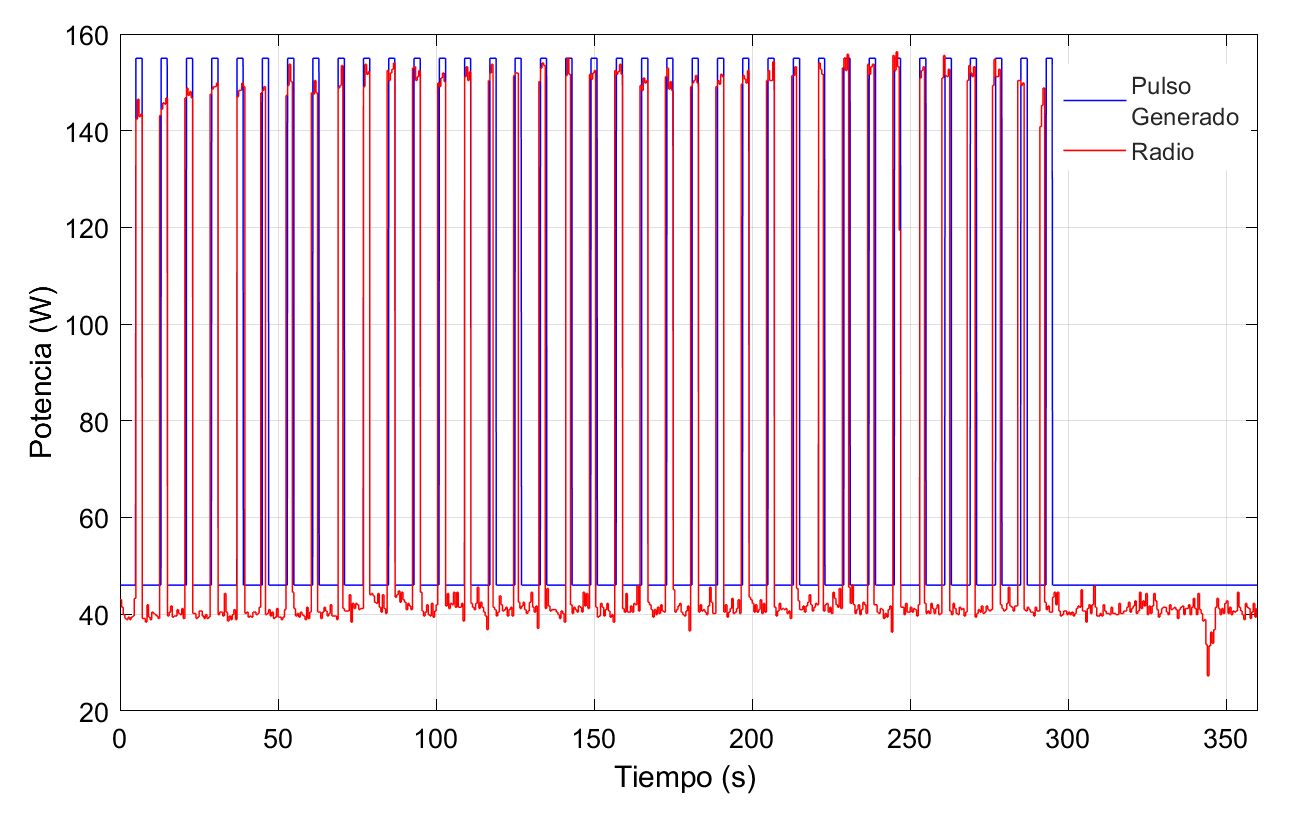
\includegraphics[scale=0.6]{Figuras/Validacion_2_P.eps}
\caption{Gráfico Potencias vs Tiempo de la segunda validación}
Fuente: Elaboración Propia
\label{validacion_2_P}
\end{figure}

\begin{figure}[H]
\centering
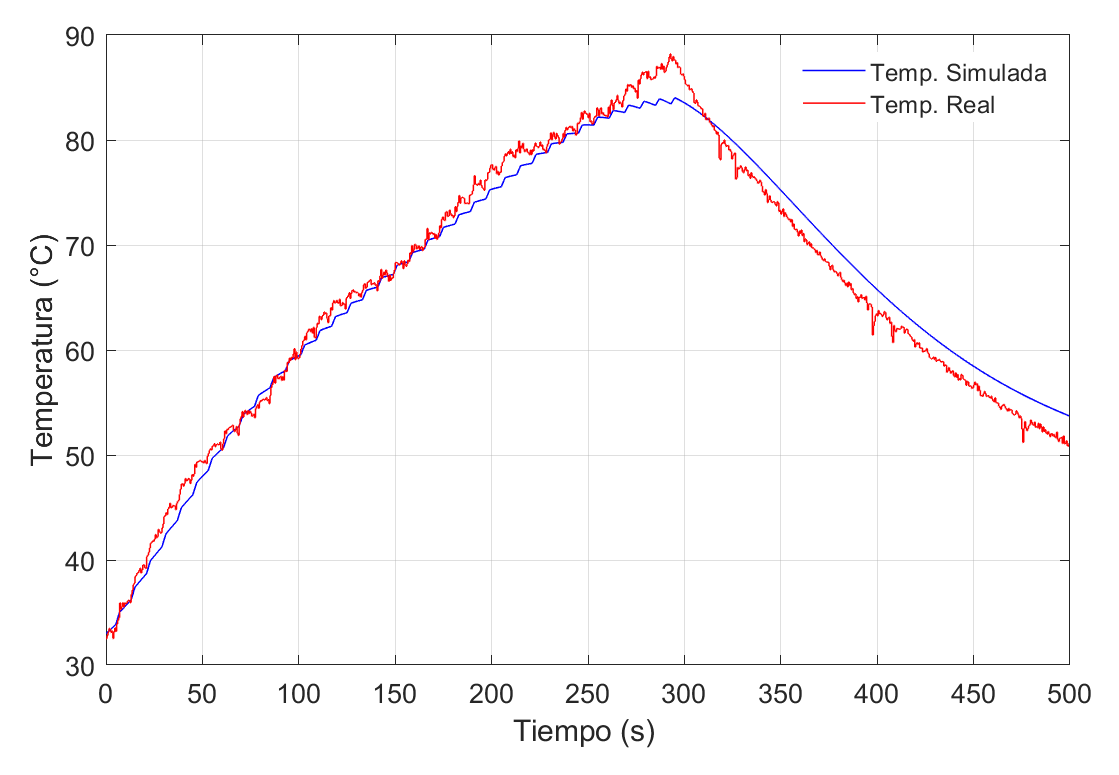
\includegraphics[scale=0.66]{Figuras/Validacion_2_T.eps}
\caption{Gráfico Temperaturas vs Tiempo de la segunda validación}
Fuente: Elaboración Propia
\label{validacion_2_T}
\end{figure}

\begin{figure}[H]
\centering
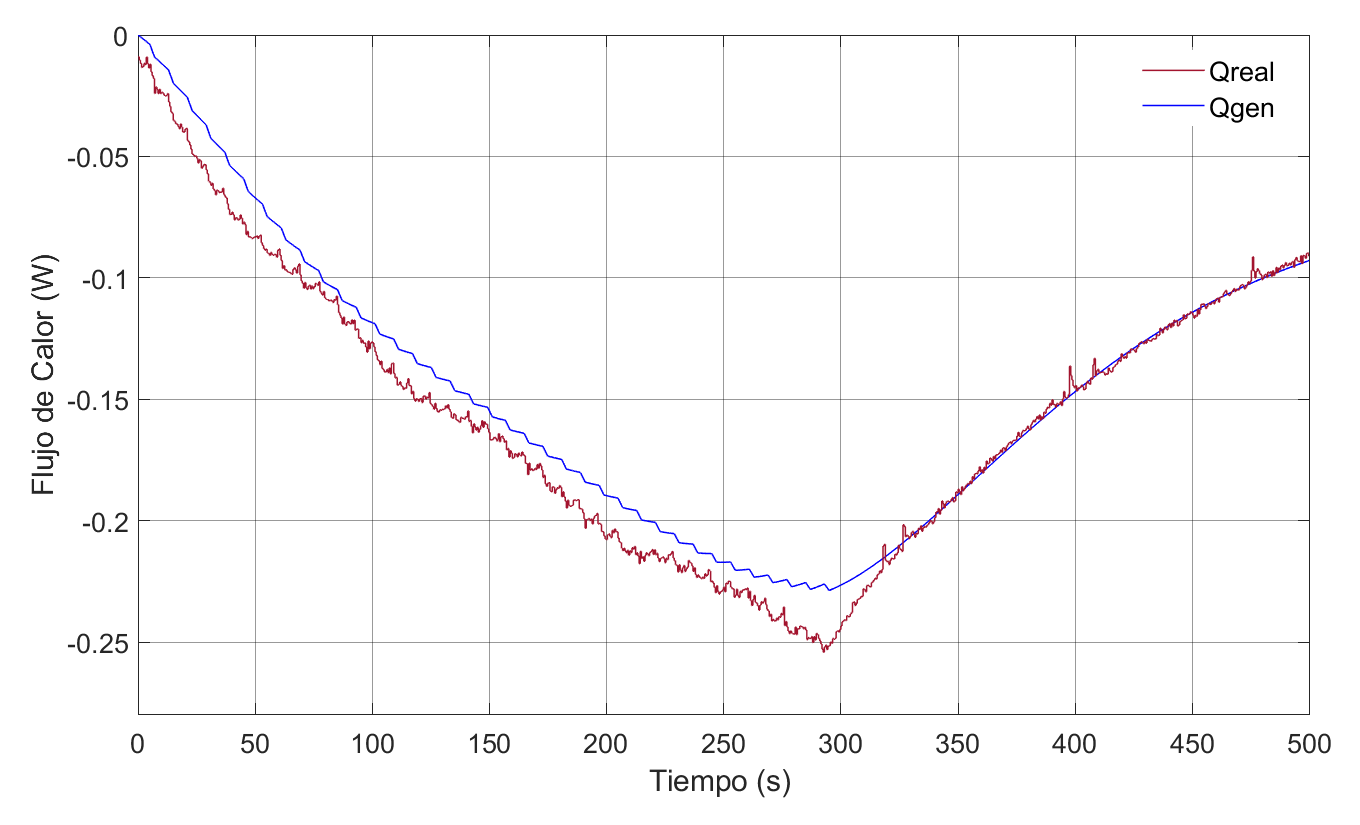
\includegraphics[scale=0.63]{Figuras/Validacion_2_Q.eps}
\caption{Gráfico Flujos de Calor vs Tiempo de la segunda validación}
Fuente: Elaboración Propia
\label{validacion_2_Q}
\end{figure}
% \chapter{Estimación de las Condiciones Operativas de la Estación Remota}

Este capítulo tiene como objetivo considerar las condiciones térmicas de la Estación Remota, dentro de su contexto operativo en Palo Verde, se toma en cuenta su interrelación con el radio transmisor y el exterior que lo rodea, para lo cual se analizarán las condiciones conocidas respecto a la ubicación futura de la estación y se unificarán nuevamente en un modelo térmico, que no solo incluya el modelo térmico del radio, sino que a su vez contemple características físicas propias de la estación y del medio en que se encuentra, de manera tal que permita tomar la mejor ruta de acción en el planteamiento de una solución.

\section{Condiciones Generales de la Estación}

\subsection{Ubicación Exacta:}

Como ya antes se mencionó, la GRT estará ubicada en el Sitio Ramsar Parque Nacional Palo Verde. El parque se encuentra aproximadamente 30 kilómetros al oeste de la ciudad de Cañas, entre el Río Bebedero y el Río Tempisque,  es un área protegida con una extensión de 16804 hectáreas y fue creada bajo el decreto ejecutivo N0.11541 el 30 de mayo de 1980 y fue ratificado por la Ley No. 6831 del 20 de diciembre de 1982. \cite{paloverde}

En la Tabla \ref{cordenadas} se muestran datos sobre la ubicación específica de la torre donde se colocará  el gabinete que contiene la GRT. Por otra parte en  la Figura \ref{ubicacion} se muestra la imagen satelital de la ubicación actual de la torre.

\begin{table}[H]
\centering
\caption{Datos de la ubicación del gabinete}
\label{cordenadas}
\begin{tabular}{cc}
\toprule
Latitud (DMS) &  10\degree20'38.2"N \\
Longitud (DMS) & 85\degree20'17.1"W \\
Altura (msnm) & 10\\
Presión Atmosférica promedio (mbar) & 1006 \\ \bottomrule
\end{tabular}
\end{table}

\begin{figure}[H]
\centering
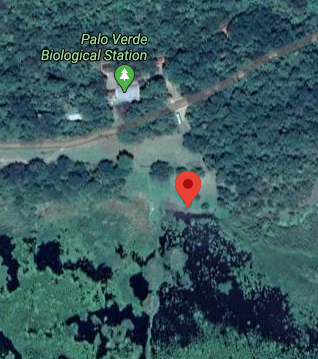
\includegraphics[scale=0.9]{Figuras/ubicacion_3.png}
\caption{Imagen Satelital de la posición de la GRT}
Fuente: Google Maps
\label{ubicacion}
\end{figure}

\subsection{Características físico-mecánicas del gabinete}

Para el montaje de los componentes internos de la GRT se hará uso de un gabinete metálico comercial, utilizado para montajes eléctricos de pared. Sus características principales se presentan en la Tabla \ref{gabinete},\cite{gabinete manual}.

\begin{table}[H]
\centering
\caption{Características del gabinete a utilizar en la GRT}
\label{gabinete}
%\begin{tabularx}{14cm}{l X}
\begin{tabular}{cc}
\toprule
\textbf{Fabricante}        & Hoffman                 \\
\textbf{Modelo}            & M600400225G             \\
\textbf{Dimensiones}       & (600x400x225) \si{\milli\meter}      \\
\textbf{Espesor de lámina} & \SI{1,2}{\milli\meter}                 \\
\textbf{Acabado} & \begin{tabular}[c]{@{}c@{}}Color Gris Claro RAL 7035 texturizado,\\ pintura poliéster en polvo por ambos lados\end{tabular} \\
\textbf{Certificaciones}   & IEC IP66 y UL Tipo 12/4 \\ \bottomrule
\end{tabular}
\end{table}

En la Figura \ref{gabinete1} se muestra un render realizado del gabinete real.

\begin{figure}[H]
\centering
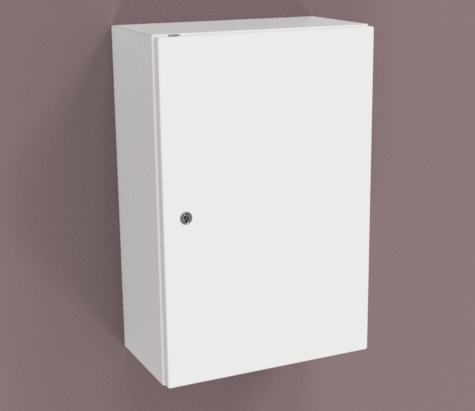
\includegraphics[scale=0.65]{Figuras/gabinete1.png}
\caption{Render del Gabinete Real}
Fuente: Elaboración Propia
\label{gabinete1}
\end{figure}

\section{Datos Meteorológicos}

Parte fundamental del modelo de la GRT implica conocer las condiciones de temperatura, radiación, dirección y velocidad del viento, que se requieren para la determinación de los diferentes parámetros termodinámicos de la simulación; para lo cual se utilizaron los datos de una estación meteorológica ubicada en la torre antes mencionada. Dichos datos eran accesibles al público a través de la OTS (\textit{Organization for Tropical Studies})\cite{ots}. Para todos los casos se recopilaron los datos de un año, comprendido entre el 1 de junio de 2019 al 1 de junio de 2020.

Los datos recopilados de la estación meteorológica, comprenden los promedios de mediciones realizadas cada 10 segundos en períodos de 15 minutos, de donde también se obtienen los valores máximos y mínimos de esos períodos de tiempo. \cite{ots}

\subsection{Temperatura}

Los datos de temperatura se organizaron en los valores correspondientes al día y los datos correspondientes a la noche, esto para no afectar el valor promedio anual de temperatura del aire, ya que para efectos del modelo es conveniente tener el valor promedio de temperatura del día, donde se espera que los valores típicos sean mayores que durante la noche.

En el caso de la resolución las regulaciones OMM (\textit{Organización Mundial de Meteorología}), indica que deben ser de \SI{0,1}{\celsius} y con una exactitud en los datos de \SI{0,2}{\celsius} , para una medición de temperatura a 1,5 metros del suelo. \cite{ots_manual}

En la Tabla \ref{temperatura_met} se muestran los datos obtenidos de la estación meteorológica para el período establecido.

\begin{table}[H]
\centering
\caption{Datos de Temperatura para el período entre 1/6/2019 y 1/6/2020}
\label{temperatura_met}
%\begin{tabularx}{12.5cm}{cccc}
\begin{tabular}{cccc}
\toprule
\multicolumn{1}{c}{\multirow{2}{*}{\textbf{Temperatura del Aire}}} & \multicolumn{3}{c}{\textbf{Valores de temperatura (\si{\celsius})}}           \\ \cline{2-4} 
\multicolumn{1}{c}{}                                & \textbf{Promedio} & \textbf{Valor máximo} & \textbf{Valor Mínimo} \\ \hline
Diurna         & 30,06 & 37,94 & 21,60 \\
Nocturna     & 26,46 & 33,88 & 21,46 \\
Día completo & 29,75 & 37,94 & 21,46 \\ \bottomrule
\end{tabular}
\end{table}

\subsection{Velocidad y Dirección del Viento}

La OMM indica que esta variable hace referencia a la velocidad del viento en superficie y para efectos meteorológicos es una cantidad vectorial compuesta por su dirección y magnitud. Su dirección se representa en grados dextrórsum, es decir en sentidos de las agujas del reloj, donde el Norte esta representado por los grados 0 y 360 y el grado 90 representa el Este. Para este caso la resolución de los datos es de 10 grados para la dirección y de 0,5 \si{\meter/\second} en la media de velocidad del viento. En cuanto a la exactitud se tiene \num{\pm\, 5}{\degree} en la dirección y \num{\pm0,5} \si{\meter/\second}\; para \SI{\leq5}{\meter/\second}; y \num{\pm10}\si{\percent}, para $>$ \SI{5}{\meter/\second}.\cite{ots_manual}


\begin{table}[H]
\centering
\caption{Valores promedios para el viento entre el período del 1/6/2019 a 1/6/2020}
\label{viento_met}
\begin{tabularx}{10cm}{c c}
%\begin{tabular}{cc}
\toprule
\textbf{Velocidad Promedio} (\si{\meter/\second}) & 3,06\\ 
\textbf{Velocidad Máxima} (\si{\meter/\second}) & 8,76\\
\hline
\textbf{Dirección Promedio (grados)} & 104,12 \\
\hline
\textbf{Desviación Estándar Promedio en la Dirección} & {22,65}  \\
\bottomrule
\end{tabularx}
\end{table}

Los valores mostrados en la Tabla \ref{viento_met} son útiles para los parámetros del modelo, por lo que los valores representados excluyen los datos de velocidad durante la noche, es por ello que en las Figuras \ref{histograma_direccion},\ref{histograma_velocidad} y \ref{rosa_de_los_vientos}, se muestran los histogramas de la dirección, la velocidad y la combinación de ambos durante las 24 horas.

\begin{figure}[H]
\centering
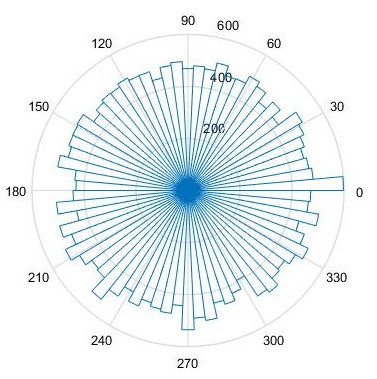
\includegraphics[scale=0.9]{Figuras/histograma_direccion.jpg}
\caption{Histograma polar de la dirección del viento}
Fuente: Elaboración Propia con datos de la OTS
\label{histograma_direccion}
\end{figure}

\begin{figure}[H]
\centering
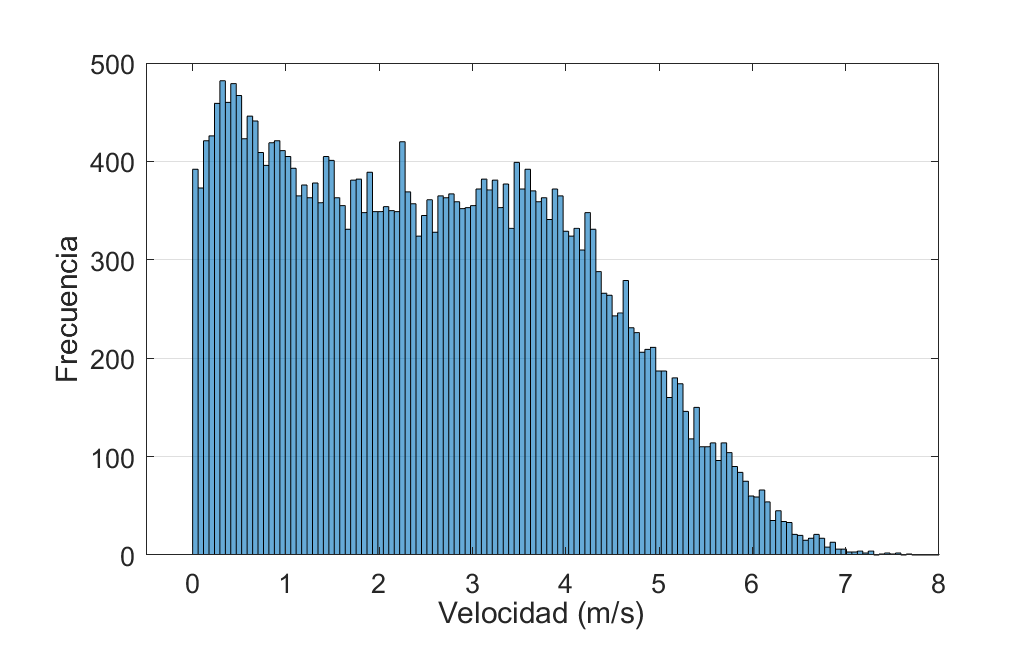
\includegraphics[scale=0.78]{Figuras/histograma_velocidad.eps}
\caption{Histograma de la velocidad del viento}
Fuente: Elaboración Propia con datos de la OTS
\label{histograma_velocidad}
\end{figure}

\begin{figure}[H]
\centering
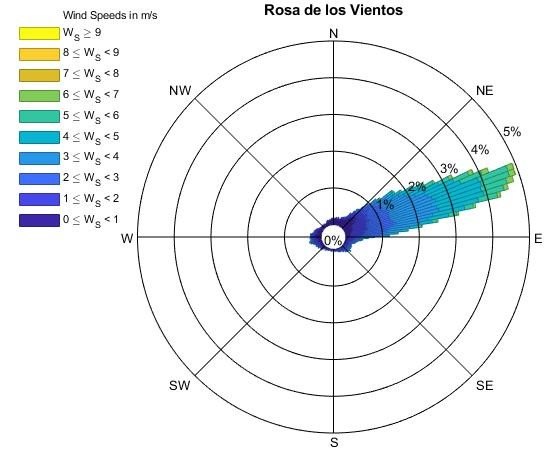
\includegraphics[scale=0.72]{Figuras/Rosa_de_los_vientos.jpg}
\caption{Histograma polar del vector viento}
Fuente: \cite{windrose} con datos de la OTS
\label{rosa_de_los_vientos}
\end{figure}

\subsection{Radiación Solar}

En la Tabla \ref{radiacion_met} se muestran los datos de radiación solar que llega a la Tierra recopilados por la estación meteorológica, en donde se tiene una resolución de \num{\pm\,1} \si{\watt/\square\meter} para los equipos de alta calidad y \num{\pm\,5}\si{\watt/\square\meter} para los de buena calidad; en cuanto a la exactitud las regulaciones de la OMM exigen \num{\pm2}\si{\percent} para la radiación global y de \num{\pm5}\si{\percent}  para la radiación neta. \cite{ots_manual}       

\begin{table}[H]
\centering
\caption{Datos de Radiación Solar entre el período del 1/6/2019 a 1/6/202 }
\label{radiacion_met}
\begin{tabular}{ccc}
\toprule
\textbf{Variable}     & \textbf{Promedio}          & \textbf{Máxima}          \\ \midrule
Radiación Solar \si{\watt/\square\meter} & \multicolumn{1}{c}{467,77} & \multicolumn{1}{c}{3361} \\ \bottomrule
\end{tabular}
\end{table}

\subsection{Humedad Relativa}

La resolución esperada de los datos para este rubro es de \SI{1}{\percent} y no más de \SI{3}{\percent} para el margen de error.\cite{ots_manual}

\begin{table}[H]
\centering
\caption{Datos de Humedad Relativa entre el período del 1/6/2019 a 1/6/202 }
\label{humedad_met}
\begin{tabular}{cccc}
\toprule
\textbf{Humedad Relativa (\si{\percent})} & \multicolumn{1}{l}{\textbf{Promedio}} & \multicolumn{1}{l}{\textbf{Máxima}} & \textbf{Mínima} \\ \midrule
Diurna                         & 63,58                                 & 98,70                               & 0,60            \\
Nocturna                       & 76,41                                 & 98,70                               & 0,51            \\ \bottomrule
\end{tabular}
\end{table}

\section{Esquema de Modelado}

La estrategia a seguir es muy similar a la utilizada para el radio transmisor, de hecho se basa en seguir el mismo esquema solamente que ampliado, consiste en tomar el modelo del radio y ampliarlo tomando en cuenta todas las condiciones termodinámicas que el radio enfrentará cuando este dentro de un gabinete en la ubicación antes descrita, y observar el comportamiento tanto del radio como de la estación y basados en estos datos obtenidos plantear una solución que se ajuste a esas condiciones operativas proyectadas.

Basado en el esquema mostrado en la Figura \ref{esquema_modelo_radio}, esta sección del proyecto consiste en ampliar el bloque referente a los \textit{Elementos Térmicos} tal y como se muestra en la Figura \ref{esquema modelo general}. Una de las suposiciones de este modelo es asumir que tanto el radio como el gabinete son dos esferas concéntricas una dentro de otra, de área superficial equivalente a sus respectivas configuraciones geométricas esto simplifica considerablemente los cálculos y procedimientos analíticos, principalmente para las estimaciones de la radiación, tal y como se vio en el marco teórico.

El objetivo es integrar el concepto de red generalizada visto en \cite{alfaro}; por otra parte en la literatura se observó que estos modos de abordar un problema de este tipo dan como resultado buenas aproximaciones en comparación de otros modelos más complejos.\cite{realtime}

\begin{figure}[H]
\centering
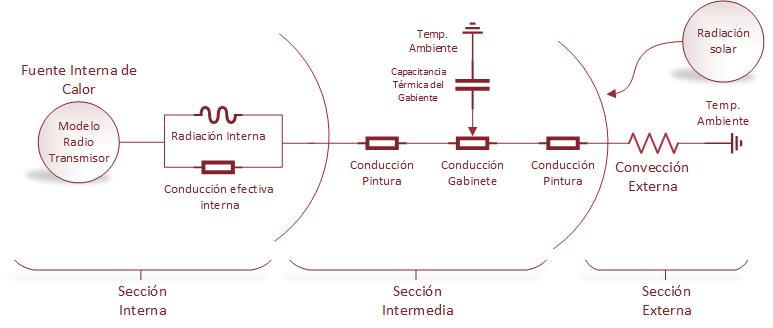
\includegraphics[scale=0.75]{Figuras/Esquema_de_Modelo_general.jpg}
\caption{Esquema de Modelo para la GRT}
Fuente: Elaboración Propia \label{esquema modelo general}
\end{figure}

\subsection{Consideraciones Generales de Simulación}

Por tratarse de una simulación termodinámica, para la resolución matemática de cada uno de los elementos involucrados se deben realizar suposiciones que permitan utilizar expresiones que dan como resultado los parámetros que se introducen dentro del software, el cual los unifica en un modelo que permite medir condiciones de flujo de calor y temperatura a través de sus diferentes secciones; dichas suposiciones se muestran a continuación

\begin{enumerate}
    \item Al igual que en el modelo del radio, se utilizarán los datos y parámetros de transmisión del experimento 2, y representar la condición más esforzada posible del radio, por la razones ya antes explicadas.
    \item Utilizar una configuración geométrica de dos esferas concéntricas, conlleva a que la fuente de calor (radio transmisor), también se considere con una posición central, esto es importante en el caso de la determinación del coeficiente de convección, debido a que los cálculos se realizaron considerando una placa en orientación vertical y no como una esfera a diferencia del resto de los cálculos; esto con el fin de determinar el coeficiente real de convección que se tendría dentro del gabinete.
    \item En las instancias en que se evalúen las propiedades del aire, se asume que el mismo se comporta como gas ideal.
    \item Para el caso de la radiación:
    \begin{itemize}
        \item Las superficies son opacas, difusas o grises, lo que implica que son emisoras y reflectoras difusas. 
        \item Las superficies son emisoras difusas con una emisividad igual al valor en la dirección normal.
        \item Sus propiedades relativas a la radiación son independientes de la longitud de onda.
        \item Cada superficie del recinto es isoterma y tanto la radiación entrante como saliente son uniformes sobre cada superficie.
        \end{itemize}
\end{enumerate}

\section{Parámetros de Simulación}

Considerando la literatura y las ecuaciones mostradas en el marco teórico a continuación se muestran los resultado de los cálculos para los parámetros de simulación a manera de tablas resumen donde se muestran los resultados del procedimiento planteado en la teoría. Para todos los casos las propiedades del aire fueron evaluadas a la presión atmosférica

\subsection{Determinación del coeficiente de convección del módulo de potencia}

\begin{table}[H]
\centering
\caption{Resultados del cálculo para la determinación del coeficiente de convección real}
\label{calculo1}
\begin{tabular}{cccc}
\toprule
\textbf{Variable} & \textbf{Valor} & \textbf{Unidad}      & \textbf{Ecuación utilizada} \\ \midrule
$T_{s}$          & 75             & \si{\celsius}          & Parámetro de diseño         \\
$T_{\infty}$ & 30 & \si{\celsius} & Parámetro de diseño \\
$A_{modulo}$ & \num{8,964e-4} & \si{\square\meter} & Parámetro constructivo \\
$T_{f}$ & 325,65 & \si{\kelvin} & \ref{tf} \\
$Ra_{L}$ & 58456,189 & $N/A$  & \ref{ra1} \\
$Nu$ & 8,079 & $N/A$& \ref{nu1}  \\
$h$ & 5,515 & \si{\watt/\square\meter\cdot\celsius} & \ref{h1} \\ \bottomrule
\end{tabular}
\end{table}

En la Tabla \ref{calculo1} se muestra la temperatura $T_{f}$ a la cual fue evaluada las propiedades del aire. Por otro lado el resultado para el coeficiente de convección difiere tan solo en un \SI{9,34}{\percent} del valor utilizado como estimación para el modelo del radio. 

\subsection{Parámetros del aire interno del gabinete}

Para esta sección el cálculo se divide en dos partes, una es el cálculo del coeficiente de conducción efectiva para el aire y la otra es la determinación de los parámetros de radiación entre dos placas. Ambos parámetros junto con el modelo del radio representan la sección interna de la estación (Figura \ref{esquema modelo general}).

\textbf{Coeficiente efectivo del aire:}

\begin{table}[H]
\centering
\caption{Coeficiente efectivo de conducción para el aire}
\label{calculo2}
\begin{tabular}{cccc}
\toprule
\textbf{Variable} & \textbf{Valor} & \textbf{Unidad}  & \textbf{Ecuación utilizada} \\ \midrule
$T_{s}$          & 75             & \si{\celsius}     & Parámetro de diseño         \\
$T_{\infty}$ & 30 & \si{\celsius} & Parámetro de diseño \\
$T_{prom}$ & 53,725 & \si{\celsius}& \ref{tprom} \\
$Lc$ & 0,521 & \si{\meter}  & \ref{lc}\\
$F_{esf}$ &  $2,89\times 10^{-5}$ & $N/A$ & \ref{fesf} \\
$Ra_{L}$ & 410450834,398  & $N/A$ & \ref{ra1}  \\
$Nu$ & 8,079 & $N/A$ & \ref{nu1}  \\
$k_{ef}$ & 0,2208 & \si{\watt/\meter\cdot\celsius} & \ref{h1}\\
\bottomrule
\end{tabular}
\end{table}

Si se compara el coeficiente de conducción del aire evaluado a la temperatura $T_{prom}$ contra el coeficiente $k_{ef}$ se tiene que este último es 8 veces más grande, de ahí radica la importancia de este cálculo para recintos cerrados.

\textbf{Radiación interna del recinto:} El software para realizar el cálculo de la radiación entre dos placas o paredes utiliza lo que denomina un factor de radiación, que se denominará en este proyecto como $k_{rad}$, el cual depende en cierta manera de la configuración geométrica de las placas; además este factor de radiación es equivalente a tomar la Ecuación \ref{radint} y reducirla a contener parte de sus términos dentro del factor antes mencionado, tal y como se muestra a continuación.

\begin{equation}\label{kradiacion}
    k_{rad}=\frac{\sigma }{\frac{1}{\varepsilon _{1}}+\frac{1-\varepsilon _{2}}{\varepsilon _{2}}\cdot \left | \frac{r_{1}}{r_{2}} \right |^{2}}\;\;(\si{\watt/\square\meter\cdot\kelvin\tothe{4}}) 
\end{equation}

En la tabla se muestran los valores de emisividad correspondientes para cada caso, cabe aclarar que en este cálculo se está considerando la radiación existente entre la superficie del módulo de potencia (considerada como una esfera) y la superficie interna del gabinete, la cual es la capa de pintura, por lo que el dato de emisividad debía ser justamente del tipo de pintura.

Debido a la dificultad de obtener un dato de emisividad para la pintura en específico que utiliza el gabinete, por lo que se utilizó el valor de pinturas con características similares y se habla de similares ya que la literatura no es concluyente respecto a si el color influye en el valor de emisividad; hay fabricantes que asocian un valor de emisividad a sus pinturas obtenidos de manera experimental, mientras que existen estudios que indican que el color de la pintura no influye en dicho factor, sino más bien la forma de aplicación, el acabado y la composición de la misma. \cite{flir},\cite{indecolor} 

\begin{table}[H]
\centering
\caption{Parámetros para el factor de radiación}
\label{calculo3}
\begin{tabular}{cccc}
\toprule
\textbf{Variable}   & \textbf{Valor} & \textbf{Unidad} & \textbf{Ecuación utilizada} \\ \midrule
$\varepsilon _{1}$ & 0,1            & $N/A$           & Parámetro constructivo      \\
$\varepsilon _{2}$ & 0,9            & $N/A$           & Parámetro constructivo      \\
$r_{1}$ & 0,0084 & \si{\meter}& $N/A$           \\
$r_{2}$  & 0,2688 & \si{\meter} & $N/A$ 
\\
$k_{rad}$ & \num{5,6699e-9} & \si{\watt/\square\meter\cdot\kelvin\tothe{4}}& \ref{kradiacion}\\
\bottomrule
\end{tabular}
\end{table}

El valor de emisivilidad para el módulo de potencia, es el de un metal pulido y los valores $r_{1}$ y $r_{2}$ son los correspondientes al radio de una esfera de un área superficial equivalente al del módulo y al gabinete respectivamente.  

\subsection{Parámetros del Gabinete}

Para la determinación de estos parámetros, se hizo uso de la herramienta de modelado CAD 3D \textit{fusion 360} para lograr determinar características físicas que no eran mencionadas dentro de las especificaciones del fabricante; el cual tampoco es muy específico en cuanto al material del gabinete, salvo de indicar que se trata de acero, por lo que se asumió para los cálculos un acero AISI 1010 y sus propiedades se obtuvieron de. \cite{cengel}

\begin{table}[H]
\centering
\caption{Características para el gabinete}
\label{calculo4}
\begin{tabular}{cccc}
\toprule
\textbf{Variable} & \textbf{Valor} & \textbf{Unidad} & \textbf{Ecuación utilizada} \\ \midrule
$A_{s}$ & 1,03643 & \si{\square\meter} & Parámetro constructivo      \\
$m$ & \num{\sim10,48} & \si{\kilogram}  & Parámetro constructivo\\
$C_{p}$ & 434 & \si{\joule/\kilogram\cdot\kelvin}& Dato de Tabla
\\
$k$ & 63,9 & \si{\watt/\meter\cdot\kelvin} & Dato de Tabla
\\
\bottomrule
\end{tabular}
\end{table}

Esta sección consta de tres elementos que se pueden agrupar en dos; uno es la determinación de la resistencia térmica conductiva tanto de la pintura como del gabinete y la determinación de la capacidad calorífica del gabinete, es decir su capacitancia térmica o capacidad de almacenar energía calórica. Estos tres elementos componen la sección intermedia de la Figura \ref{esquema modelo general}.

\textbf{Resistencia térmica del gabinete y pintura:} Una forma de estimar la transferencia de calor a través de una pared de espesor $L$, es utilizando la analogía eléctrica de la resistencia y observar esta pared como un elemento que se opone al flujo de calor de modo que se puede obtener una expresión como la siguiente para determinar la resistencia térmica. \cite{cengel}

\begin{equation}\label{resistencia}
    R_{cond}=\frac{r_{2}-r_{1}}{4\pi  r_{1}r_{2}\cdot  k}\;\;(\si{\celsius/\watt})
\end{equation}
 
Donde: 

\begin{itemize}
    \item $r_{1}$ es el diámetro interno de pared (\si{\meter})
    \item $r_{2}$ es el diámetro externo de pared (\si{\meter})
    \item $k$ es el coeficiente de conductividad térmica (\si{\watt/\meter\cdot\kelvin})
\end{itemize}

Los valores $r_{1}$ y $r_{1}$ se pueden determinar fácilmente con el espesor de lámina del gabinete y del cálculo de radio equivalente para el área superficial del gabinete. Tomando eso en consideración en la Tabla \ref{calculo5} se muestran los resultados obtenidos para  las resistencias térmicas.\cite{cengel}

\begin{table}[H]
\centering
\caption{Resistencias térmicas para la sección intermedia}
\label{calculo5}
\begin{tabular}{cccc}
\toprule
\textbf{Variable} & \textbf{Valor}                                        & \textbf{Unidad} & \textbf{Ecuación utilizada}        \\ \midrule
$R_{gabinete}$   & \num{1,886e-5} & \si{\celsius/\watt}  & \ref{resistencia} \\
$R_{pintura}$    & 0,1707  & \si{\celsius/\watt}  & \ref{resistencia} \\ \bottomrule
\end{tabular}
\end{table}

\textbf{Capacitancia térmica del gabinete:} Este bloque el software lo representa como la capacidad del cuerpo para almacenar energía en forma de calor considera su masa y calor específico, el cálculo lo realiza el software mediante la siguiente ecuación. Los valores asociados a la Ecuación \ref{thermal mass} se encuentran especificados en la Tabla \ref{calculo4}.

\begin{equation}\label{thermal mass}
    Q=c\cdot m\frac{dT}{dt}\;\;(\si{\watt})
\end{equation}

Donde:

\begin{itemize}
    \item $c$ es el calor específico (\si{\joule/\kilogram\cdot\kelvin})
    \item $m$ es la masa (\si{\kilogram})
\end{itemize}

\subsection{Parámetros externos}

Como su nombre lo indica, corresponde a los parámetros correspondientes a la sección externa del esquema de modelo, compuesta por los elementos que describen el coeficiente de convección externa y la estimación de la radiación entrante en el gabinete.

\textbf{Coeficiente de convección externa:} Para este cálculo se utilizaron los datos de velocidad del viento de la Tabla \ref{viento_met}. Además se establecen los parámetros de temperatura del aire y temperatura promedio externa del aire para la evaluación de las propiendas del aire.

\begin{table}[H]
\centering
\caption{Cálculos del coeficiente de convección externa}
\label{calculo6}
\begin{tabular}{cccc}
\toprule
\textbf{Variable} & \textbf{Valor}  & \textbf{Unidad}      & \textbf{Ecuación utilizada} \\ \midrule
$T_{aire}$ & 30,45  & \si{\celsius} & Parámetro ambiental \\
$T_{prom}$ & 29,97 & \si{\celsius} & Parámetro ambiental
\\
$Nu$ & \num{1,886e-5} & $N/A$ & \ref{nu2} \\
$Re$ & 0,1707 & $N/A$ & \ref{re2}\\
$h$ & 14,5728 & \si{\watt/\square\meter\cdot\celsius} & \ref{hext} \\
\bottomrule
\end{tabular}
\end{table}

\textbf{Determinación Radiación Solar:} En cuanto a la radiación, el modelo contempla este dato como una fuente de calor aplicada a la mitad del área de una esfera, ya que bajo esta simplificación la radiación sin importar la posición del sol siempre irradiará la mitad de la esfera, por lo que quedaría considerar simplemente el momento del día en el cual la radiación es más intensa, y esto es de esperarse en horas del medio día según los datos de la OTS.

Para determinar la magnitud de esta fuente de calor existían dos posibilidades: una consiste en utilizar los datos meteorológicos, y el otro en realizar los cálculos demostrados en la teoría apoyados con la utilización de un algoritmo de posición solar implementado por la National Renewable Energy Laboratory (NREL) el cual permite considerar la ubicación exacta del lugar, parámetros de presión atmosférica, altitud, incluso realizar una estimación para una fecha y hora en específico \cite{spa} . En la Tabla \ref{comparacion radiacion} se muestra una comparación para la fecha y hora indicadas entre los datos meteorológicos y los resultados obtenidos de los cálculos realizados con base en la teoría y con el soporte del algoritmo.

\begin{table}[H]
\centering
\caption{Comparativa entre las estimaciones para la radiación solar}
\label{comparacion radiacion}
\begin{tabular}{ccc}
\toprule
\textbf{Herramienta} & \textbf{Valor (\si{\watt/\square\meter})} & \textbf{Fecha y hora de evaluación}       \\ \midrule
Algoritmo & 1036,4 & \multirow{2}{*}{4 de mayo de 2020 a las 12:15 pm} \\
Datos Meteorológicos & 1054 &             \\
\bottomrule
\end{tabular}
\end{table}

La diferencia entre los dos métodos para esta fecha y hora en específico es de apenas \SI{1,68}{\percent}, sin embargo cuando se trata de cálculos de radiación solar se debe tener especial cuidado, ya que el hecho de que exista una nube en el momento de la medición, para el caso del dato meteorológico, cambia completamente el dato mostrado y la variación podría ser significativa. Es por esta razón que se decide implementar el cálculo de radiación solar mediante el algoritmo, y utilizar el valor mostrado en la Tabla \ref{comparacion radiacion}, ya que este permite realizar estimación de radiación para fechas especificas y sobre superficies con diferentes ángulos de inclinación en caso de ser necesario, lo cual le atribuye la ventaja de  poderse utilizar para modelos de estaciones en otras ubicaciones geográficas también.

Para el caso especifico de la GRT en Palo Verde se recomienda, siempre y cuando se pueda, realizar la comparación entre los dos métodos en la evaluación de fechas pasadas de manera que se tenga una estimación más fiable de la radiación, principalmente su alta desviación estándar en las mediciones. En el Apéndice se muestra el dato de la OTS usado en la Tabla \ref{comparacion radiacion}.

\textbf{Humedad:} Como es de esperar los valores de humedad relativa durante el día son elevados, alrededor de \SI{70,32}{\percent} promedio durante el período evaluado para los demás parámetros. Al utilizar la Ecuación \ref{calculo td} para estimar la posibilidad de condensación en el gabinete, se observó que las horas nocturnas presentaban el mayor riesgo, ya que en ocasiones tenían valores de temperatura de rocío cercanos a la temperatura ambiente. Sin embargo, al igual que en el caso de la radiación, los parámetros de humedad relativa tienen una alta variabilidad en el tiempo más aún que depende de factores como la temperatura ambiente y la presión atmosférica.


\section{Resultados de Simulación}

Para todas la simulaciones realizadas, se partía de la suposición de un día claro al medio día, con valores promedio de temperatura y velocidad del viento diurnas constantes para un lapso de \SI{850}{\second}. Para el caso de los valores de temperatura mostrados en las Figura \ref{gabinete t}, se muestran las temperaturas obtenidas de la simulación en contraste con los datos de temperatura real, a manera de punto de referencia para la comparación. Por otra parte, en la Figura \ref{gabinete q} se observa el flujo de calor entregado por el radio hacia el gabinete. En el Anexo \ref{anexo10} se muestra el algoritmo construido para la obtención de los resultados.

\begin{figure}[H]
\centering
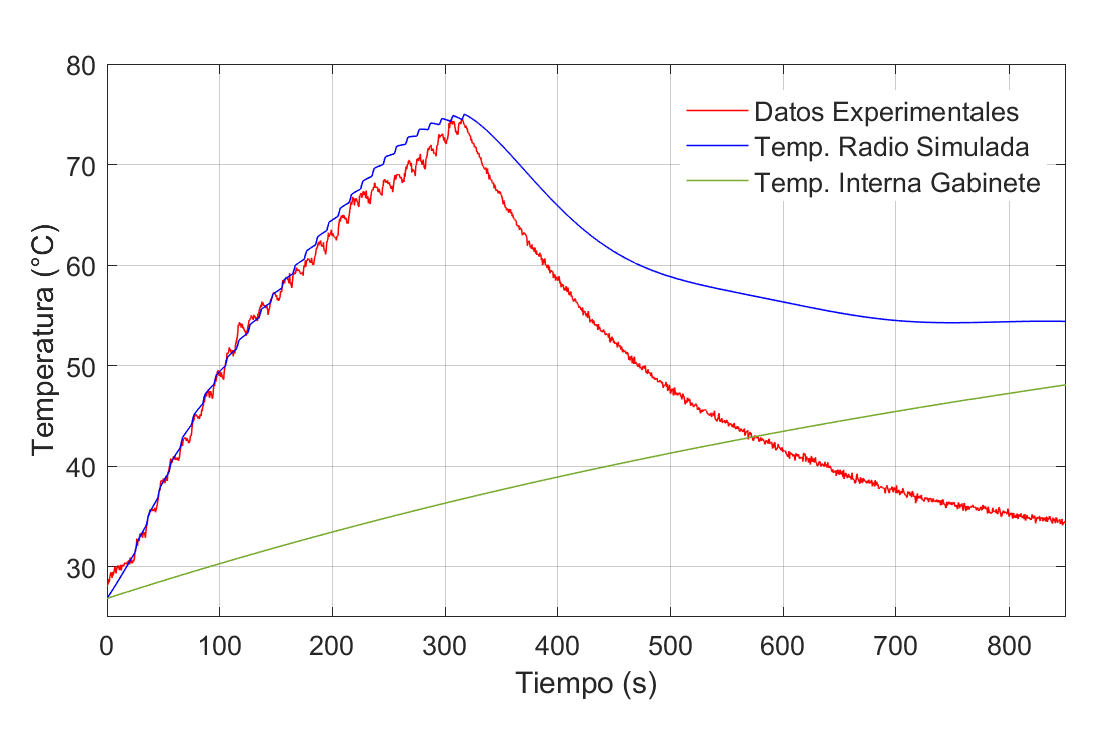
\includegraphics[scale=0.7]{Figuras/Gabinete_T.eps}
\caption{Gráfica Temperaturas vs tiempo}
Fuente: Elaboración Propia \label{gabinete t}
\end{figure}

\begin{figure}[H]
\centering
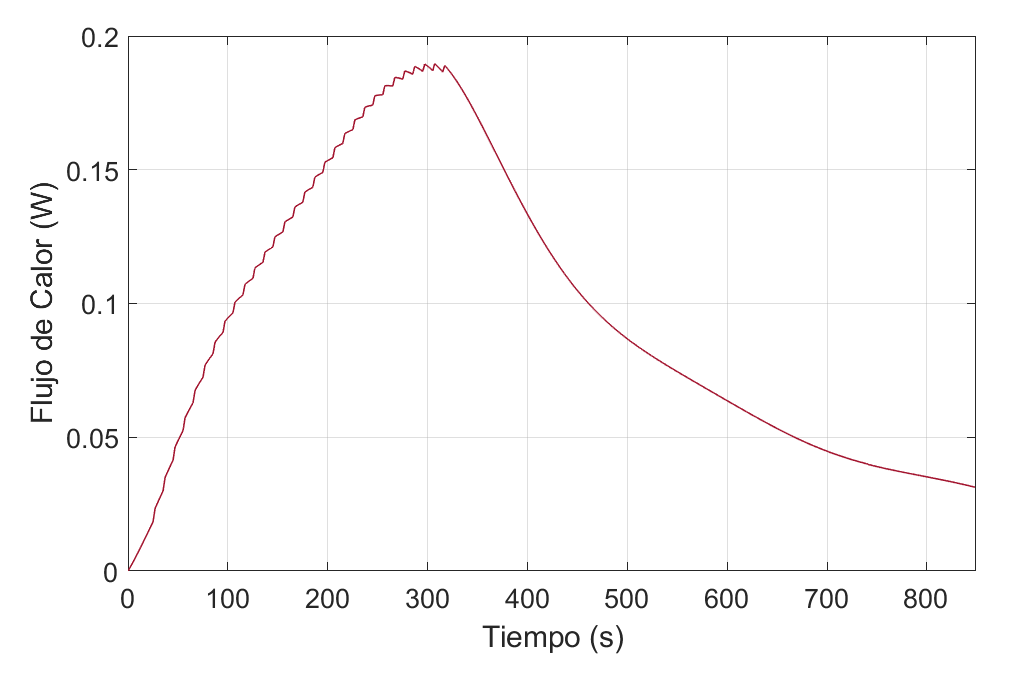
\includegraphics[scale=0.75]{Figuras/Gabinete_Q.eps}
\caption{Gráfica de Flujo de calor vs tiempo}
Fuente: Elaboración Propia \label{gabinete q}
\end{figure}

\subsection{Análisis de Resultados}

De los datos obtenidos se extraen las siguientes observaciones.

\begin{enumerate}
    \item En la Figura \ref{gabinete t} se observa como el perfil de temperatura para el radio, se ve afectado luego de que finaliza la transmisión, donde la temperatura de estabilización se alcanza aproximadamente a los \SI{55}{\celsius}; en este punto es donde la radiación solar afecta el módulo de potencia en el caso de que el mismo no posea un disipador.
    \item La temperatura interna del gabinete de la Figura \ref{gabinete t} representa en el modelo la temperatura entre el aire interno del gabinete y la capa interna de pintura del mismo. De igual manera que para el módulo de potencia, presenta una elevación de temperatura a una tasa aproximada de \SI{1,5}{\celsius/\min} donde la temperatura de equilibrio térmico de la estación estaría aproximadamente a los \SI{55}{\celsius}.
    \item Si bien es cierto la temperaturas observadas se acercan al punto de operación máximo para el radio transmisor, se debe considerar que el flujo de calor por radiación simulado es constante, lo cual no sucede en la realidad, como ya se mencionó los datos observados de radiación de la estación meteorológica indican una gran variabilidad de este valor en intervalos incluso de \SI{15}{\min} y con desviaciones estándar muy elevadas sin embargo, el valor de radiación utilizado representa un valor promedio de radiación para la zona, por lo que sus efectos en la GRT no deben ser despreciados.
    \item Como era de esperarse el flujo de calor por parte del radio hacia el gabinete se observa que no varia respecto al modelo del radio, salvo que en esta ocasión el valor es positivo porque en el contexto del modelo el sistema es el gabinete como tal por lo tanto la energía es entregada por el radio hacia el sistema.
\end{enumerate}


% \chapter{Diseño Termo-mecánico}

El presente capítulo tiene como propósito, utilizar la información y análisis recopilados a través de los capítulos anteriores para proponer una solución térmico-mecánica integral para el radio y la GRT, en consideración de todos los aspectos operativos actuales y deseados para la estación. Como su nombre lo indica la propuesta consta de dos parte fundamentales, la primera hace referencia a la solución térmica-pasiva propuesta, la cual se relaciona directamente con la parte mecánica, debido a la necesidad de adaptar un dispositivo electrónico a condiciones mecánicas y térmicas adversas a su diseño original.

\section{Contexto mecánico del radio}

Como ya antes se ha mencionado el radio es un dispositivo electrónico comercial  que se tiene que ajustar para otras condiciones como por ejemplo, su adaptación estructural dentro del gabinete. Para lo cual se debió realizar un modelo en 3D que permitiera el manejo del mismo dentro del espacio del gabinete.

\begin{figure}[H]
\centering
\includegraphics[scale=0.6]{Figuras/G5.png}
\caption{Render del Radio transmisor}
Fuente: Elaboración Propia
\label{G5}
\end{figure}

Una de las principales preocupaciones estructurales es asegurar el libre acceso a los módulos de potencia, sin comprometer la integridad del radio ni el acceso a los puertos que son requeridos para el manejo del radio durante las transmisiones. En la Figura \ref{G1} se muestra la disposición actual de los demás componentes de la estación diseñados hasta el momento. En los Anexos \ref{anexo16},\ref{anexo17},\ref{anexo18} y \ref{anexo19} se muestran imágenes reales del radio y su configuración física original. 

\begin{figure}[H]
\centering
\includegraphics[scale=0.6]{Figuras/G1.png}
\caption{Render del estado actual de la GRT}
Fuente: Render de elaboración propia con datos del SETECLab
\label{G1}
\end{figure}

\begin{figure}[H]
\centering
\includegraphics[scale=0.75]{Figuras/gabinete2.jpg}
\caption{Acceso inferior del gabinete}
Fuente: \cite{gabinete manual}
\label{acceso}
\end{figure}

Como se observa en las Figuras \ref{G1} y \ref{acceso} el gabinete cuenta con un acceso inferior para los cables, el mismo será el único utilizado tanto para el disipador como para el conector de la antena. Este último elemento es de vital importancia en la transmisión de los datos, lo que implica que la distancia entre el conector y el radio debe ser la mínima. Todas estas consideraciones convergen en la decisión de colocar el radio transmisor en la parte inferior del gabinete tal y como se muestra.

\begin{figure}[H]
\centering
\includegraphics[scale=0.6]{Figuras/G3.png}
\caption{Montaje del radio}
Fuente: Elaboración Propia
\label{G3}
\end{figure}

\begin{figure}[H]
\centering
\includegraphics[scale=0.6]{Figuras/G4.png}
\caption{Vista General del Montaje}
Fuente: Elaboración Propia
\label{G4}
\end{figure}


En las Figuras \ref{G3} y \ref{G4} se logra apreciar como la placa secundaria (Figura \ref{secundaria}) se giro 90 grados con respecto a la placa principal (Figura \ref{principal}). Esto da solución al inconveniente de no poder separar las dos placas debido a los cables de comunicación que las unen entre sí y dan acceso libre a los módulos de potencia. Se debe recordar que el módulo en estudio es el marcado como $UHF$ en las distintas figuras.

\section{Propuesta de diseño}

Una vez conocida la posición del radio dentro del gabinete, se hace uso del recurso del modelo de la estación para plantear una solución térmica pasiva que mejore las condiciones operativas de la estación y del radio transmisor. En este punto del proyecto, la parte del modelo y la parte mecánica están estrechamente relacionadas, por lo que se echará mano a los recursos computacionales para optimizar los cálculos.

\subsection{Diseño de disipador}

Desde el punto de vista mecánico el disipador debe cumplir con las siguientes condiciones:

\begin{enumerate}
    \item No debe agregar fuerzas de tracción o de palanca sobre los módulos de potencia, los cuales están diseñados para una disposición horizontal no vertical.
    \item El disipador debe ser capaz de aprovechar las corrientes de aire desde cualquier dirección, ya que, como se observó en los datos meteorológicos la dirección del viento es muy variable y no se puede garantizar aún la posición del GRT sobre la torre, de manera que se desconoce si dicha ubicación concuerda con la dirección de las ráfagas de mayor intensidad.
    \item El disipador en general debe ser de fácil montaje, desmontaje, y construcción, de manera que pueda ser construido y ensamblado por los mismos estudiantes o integrantes del laboratorio 
\end{enumerate}

\textbf{Estimación del área mínima de transferencia para el disipador:} Utilizando la Ecuación \ref{Newton} de la ley de enfriamiento de Newton, se puede realizar una estimación del área superficial de transferencia con la suposición válida de que el coeficiente de convección es constante durante el proceso y que la temperatura en la superficie de las aletas del disipador es regular en toda la superficie. \cite{cengel}

Durante los experimentos se observó que el flujo del calor del radio hacia el medio no superaba los \SI{0,3}{\watt}, por lo que la estimación del área mínima de convección se estimará con un flujo de calor de \SI{0,5}{\watt} a manera de factor de seguridad. Por lo tanto

\begin{equation}\label{area minima}
    A=\frac{Q}{h(T_{s}-T_{\infty })}\;\;(\si{\watt})
\end{equation}

Donde los valores utilizados para las variables son:

\begin{table}[H]
\centering
\caption{Estimación del área mínima}
\label{calculo20}
\begin{tabular}{cccc}
\toprule
\textbf{Variable} & \textbf{Valor}  & \textbf{Unidad}      & \textbf{Ecuación utilizada} \\ \midrule
$Q$ & 0,5  & \si{\watt} & Parámetro de diseño \\
$h$ & 14,57 & \si{\watt/\square\meter\celsius} & Parámetro de diseño
\\
$T_{s}$ & 40 & \si{\celsius}& Parámetro de diseño\\
$T\infty$ & 30,45 & \si{\celsius} & Parámetro ambiental\\
\bottomrule
\end{tabular}
\end{table}

Se obtiene un área mínima de:

\begin{equation}\label{resultado area}
    A_{min}= 3,59\times 10^{-3}\;(\si{\square\meter})
\end{equation}

El resultado obtenido parte de la suposición de que el disipador estará a la temperatura superficial mostrada como parámetro de diseño de punto de operación para el módulo, por ende una área menor a la calculada implica una temperatura igual o mayor a las que el radio alcanza actualmente. Si utilizáramos el área mínima obtenida y lo extendiéramos en una superficie cuadrada, se obtendría un cuadrado de aproximadamente $6X6$ \si{\centi\meter}, lo cual es relativamente pequeño.

\textbf{Propuesta de Disipador:} Considerando la manufactura del disipador se optará por una geometría cilíndrica vertical, a diferencia de las configuraciones rectangulares tradicionales; esto debido a que desde el punto de vista de manufactura, una barra cilíndrica es más fácil de maquinar que una rectangular; por otro lado desde el punto de vista de transferencia de calor, esta geometría permite aprovechar las ráfagas de viento provenientes de cualquier dirección independientemente de la orientación de la estación en la torre.

\begin{figure}[H]
\centering
\includegraphics[scale=0.6]{Figuras/heat_sink.png}
\caption{Propuesta de disipador}
Fuente: Elaboración Propia
\label{heat_sink}
\end{figure}

Por facilidades constructivas para el diseño se propone utilizar una barra de aluminio de $1\,in$ (\SI{25,40}{\milli\meter}) y realizar reducciones con un torno convencional a diámetros internos de $1/4\,in$ (\SI{6,35}{\milli\meter}), dándole así forma a las aletas de (\SI{3}{\milli\meter}) de espesor. El espaciado entre las mismas se determina según lo analizado en el marco teórico

\begin{table}[H]
\centering
\caption{Distanciamiento Óptimo para las aletas}
\label{resultado_sopt}
\begin{tabular}{cccc}
\toprule
\textbf{Variable} & \textbf{Valor} & \textbf{Unidad} & \textbf{Ecuación utilizada} \\ \midrule
$Ra_{L}$ & \num{1,3176e4} & $N/A$ & \ref{ra1}           \\
$L$  & 0,0254               & \si{\meter}   & Parámetro de diseño \\
$S_{opt}$   & 0,0068  & \si{\meter} & \ref{sopt}    \\
$n$ & 7 & $N/A$ & \ref{numeroaletas}        \\ \bottomrule
\end{tabular}
\end{table}

Al realizar el diseño mostrado en la Figura \ref{heat_sink} se obtuvo finalmente una área superficial real de \num{6,57e-3}\si{\square\meter}, lo cual es \num{1,83} veces más que el área mínima; sin embargo como se observó en el modelo de la estación, la radiación solar tiene un impacto significativo en la temperatura interna del gabinete por lo que para efectos del proyecto se utilizarán dos de estos disipadores, con el fin minimizar este impacto de la estación sobre el radio.

Considerando todos estos aspectos, la ubicación del radio en la estación y la geometría y ubicación de los módulos de potencia se realiza la siguiente propuesta de disipador.

\begin{figure}[H]
\centering
\includegraphics[scale=0.6]{Figuras/heat_sink_completo.png}
\caption{Propuesta completa de disipador}
Fuente: Elaboración Propia
\label{heat_sink_completo}
\end{figure}

Con la propuesta mostrada en la Figura \ref{heat_sink_completo} se pretende abarcar los dos módulos de potencia mediante las placas horizontales, darle un camino al flujo de calor mediante las dos barras que las atraviesa, y llegar a una base que sirve de soporte dentro del gabinete, pero a la vez de conexión con el exterior y los disipadores. Más adelante se detalla su interfaz con el radio transmisor y con el gabinete. Por otro lado los planos constructivos se encuentran en los anexos

\section{Modelo térmico del disipador:}

El esquema de modelado para esta ocasión, consiste en partir del modelo para la estación y agregarle los bloques y parámetros que simulen el comportamiento térmico del disipador y determinar el impacto que el mismo tendría en el radio y la estación.

\textbf{Pasta térmica:} Para efectos de cálculos, por lo general cuando se trata de transferencia de calor por conducción , se asume que las superficies en contacto son lisas, lo cual en la realidad no es cierto; la rugosidad del material genera un efecto conocido como resistencia de contacto, y esta asociada a las pequeñas burbujas de aire que se forma entre las rugosidades de ambos materiales. Este efecto no suele ser despreciable para situaciones como esta sin embargo, su determinación suele ser experimental y complicada de realizar. \cite{cengel}

Los módulos de potencia por su parte poseen superficies pulidas con el fin de reducir este efecto y como sucede en la mayoría de estos casos se hace uso de una pasta térmica, la cual genera una capa uniforme conductora de calor, que elimina estas pequeñas burbujas y crea una interfaz entre las rugosidades de ambos materiales. La pasta térmica a utilizar posee un coeficiente de conductividad térmica de: \cite{pasta}

\begin{equation}\label{kpasta}
    k_{pasta}=1,172\;\;(\si{\watt/\meter\cdot\kelvin})
\end{equation}

\textbf{Barras conductoras:} Como se muestra en la Figura \ref{heat_sink_completo} las barras representan un medio de transferencia entre la interfaz módulo-placa y la interfaz base-disipador por lo que se debe considerar la conducción térmica a través de las mismas, para lo cual se utilizan las propiedades para el Aluminio 60661-T6; el diámetro de estas barras es de$1/4\,in$ (\SI{6,35}{\milli\meter}).

\begin{table}[H]
\centering
\caption{Parámetros para la conductividad de las barras}
\label{barras}
\begin{tabular}{cccc}
\toprule
\textbf{Variable} & \textbf{Valor}          & \textbf{Unidad} & \textbf{Ecuación utilizada} \\ \midrule
$k_{Al}$& 167 & \si{\watt/\meter\cdot\kelvin} &\cite{aluminio}      \\
$A_{total}$ & \num{2,53355e-4} & \si{\square\meter} & Parámetro de diseño   \\ \bottomrule
\end{tabular}
\end{table}

Para efectos del modelo la parte de convección externa, se utilizará el mismo bloque empleado en el modelo de la estación con la corrección respectiva en el área superficial de transferencia.

\subsection{Resultados del modelo térmico}

A partir de la experiencia del modelo de la estación, se propuso realizar dos casos de simulación, en donde se varié la radiación para observar su impacto tanto en el radio como en la estación. En el primer caso se utiliza el valor de radiación usado para el modelo de la GRT (caso \SI{100}{\percent} radiación); y un segundo caso en donde se reduce la radiación en un \SI{50}{\percent} de la utilizada.

\textbf{Caso 1}

\begin{figure}[H]
\centering
\includegraphics[scale=0.65]{Figuras/disipador_T.eps}
\caption{Gráfico temperatura vs tiempo para el modelo del disipador}
Fuente: Elaboración Propia
\label{disipador T}
\end{figure}

\begin{figure}[H]
\centering
\includegraphics[scale=0.75]{Figuras/disipador_Q.eps}
\caption{Gráfico Flujo de calor vs tiempo del disipador}
Fuente: Elaboración Propia
\label{disipador Q}
\end{figure}

\begin{figure}[H]
\centering
\includegraphics[scale=0.75]{Figuras/disipador_comparacion.eps}
\caption{Gráfico comparativo de la temperatura interna del gabinete}
Fuente: Elaboración Propia
\label{disipador comparacion}
\end{figure}

\textbf{Caso 2}

\begin{figure}[H]
\centering
\includegraphics[scale=0.68]{Figuras/disipador_T_2.eps}
\caption{Gráfico temperatura vs tiempo para el modelo del disipado para el segundo caso}
Fuente: Elaboración Propia
\label{disipador T2}
\end{figure}

\begin{figure}[H]
\centering
\includegraphics[scale=0.69]{Figuras/disipador_Q_2.eps}
\caption{Gráfico Flujo de calor vs tiempo del disipador para el segundo caso}
Fuente: Elaboración Propia
\label{disipador Q2}
\end{figure}

\begin{figure}[H]
\centering
\includegraphics[scale=0.75]{Figuras/disipador_comparacion_2.eps}
\caption{Gráfico comparativo de la temperatura interna del gabinete para el segundo caso}
Fuente: Elaboración Propia
\label{disipador comparacion2}
\end{figure}

\subsection{Análisis del Resultado}

De la propuesta de diseño y de las simulaciones presentadas se pueden extraer las siguientes observaciones:

\begin{enumerate}
    \item Si se analiza el comportamiento del módulo de potencia, en cualquiera de los dos casos el disipador representa una mejoría notable en el comportamiento térmico del radio.
    \item En la Figura \ref{disipador comparacion} se observa como el gabinete presenta una leve mejoría debido al disipador, aún cuando este no esta dimensionado en función del manejo de la radiación.
    \item Cuando se compara el primer caso con el segundo, se ratifica la relevancia que tiene la radiación en el comportamiento térmico de la estación, y esto se observa claramente en la Figura \ref{disipador comparacion2} donde al reducir la radiación en un \SI{50}{\percent}, la temperatura tanto de gabinete como del radio se reduce significativamente.
    \item Basado en la observación anterior, se plantea la necesidad de una solución de carácter externo a la estación que reduzca el impacto o el porcentaje de radiación que llega al gabinete, como por ejemplo una estructura que genere sombra sobre el gabinete.
    \item En los dos casos se logra mantener el módulo de potencia dentro del rango operativo del mismo, de igual manera sucede con el punto de operación del radio en general. A pesar de que se observe  una tendencia a la alza en tiempo donde es difícil determinar su punto de estabilización, se debe recordar que desde el punto de vista real, los valores de radiación no se mantienen constantes, estos están en continuo aumento y disminución con respecto al promedio y varían significativamente entre periodos de \SI{15}{\min} según los datos de la estación de la OTS.
    \item A pesar de que el disipador amortigua el calentamiento del radio, una vez finalizada la transmisión se observa como debido a la radiación, el módulo sigue aumentando la temperatura en concordancia con los demás elementos y en dirección del equilibrio térmico.
    \item En cuanto a los flujos de calor, en ambos casos se superan los valores necesarios estimados para el módulo, y por el contrario se observa que dentro de la capacidad de los disipadores, estos asumen progresivamente la carga térmica del aire interno del gabinete.
    \item El valor negativo en los flujos de calor indica, para el inicio de la simulación según las condiciones internas del gabinete, que existe un diferencial de temperatura inverso a la dirección deseada del calor, tal y como se observa en las Figuras \ref{disipador comparacion} y \ref{disipador comparacion2}; conforme se da el aumento de temperatura el flujo de calor se invierte en la dirección deseada de adentro hacia afuera. Esto marca una de las implicaciones del disipador, ya que en momentos donde la temperatura ambiente sea mayor a la interior el flujo de calor se invertirá, por lo que el disipador siempre funcionará como un estabilizador térmico.
\end{enumerate}

\section{Validación del Diseño}

Para la validación tanto del diseño como del modelo para el disipador, se hizo uso de la herramienta de simulación de $Fusion 360$, la cual a parte de una validación, permite tener una mejor aproximación del comportamiento térmico del disipador y de cada uno de sus elementos que por una u otra razón no pudieron ser incluidos dentro del modelo. El software utiliza la resolución por medio de diferencias finitas, esto implica que se debe definir un tamaño de malla, entre más fina sea la malla, se aprecian mejor los cambios a través de los elementos. Para este caso se específicá un tamaño de malla de \SI{1}{\milli\meter}.

La simulación contempla al radio como una rampa de calor interno asociado a una temperatura en la placa superior, en el caso de las barras se considera un calor interno constante a manera de conducción al igual que para la base y finalmente en los disipadores se aplicó las condiciones de calor interno, convección y radiación desde el disipador hacia el exterior. Para la rampa de calor interno el parámetro inicial es una temperatura ambiente de \SI{30,45}{\celsius} a \SI{0}{\watt} con una condición final de \SI{75}{\celsius} a \SI{0,2}{\watt}, lo cual representa aproximadamente el comportamiento del radio en el modelo de la estación.

Debido a características propias del modelo donde solo se incluye el disipador y a la dificultad de agregar los demás elementos de la estación, esta simulación no se incluye la radiación solar ni la relación del disipador con respecto al gabinete.

\begin{figure}[H]
\centering
\includegraphics[scale=0.71]{Figuras/simulacion_1.png}
\caption{Resultados de la simulación en Fusión 360}
Fuente: Elaboración Propia
\label{simulacion1}
\end{figure}

Los puntos marcados en las Figuras \ref{disipador T} y \ref{disipador T2}, se colocaron para poder realizar la comparación con la Figura \ref{simulacion1}, ya en ese punto es donde la transmisión del radio finaliza y se obtiene la máxima temperatura posible entregada por el flujo del calor proveniente del módulo de potencia, en este punto se observa que tanto para el modelo como para la simulación las temperaturas son próximas entre sí, tanto para la placa del módulo como para el disipador, en este caso la simulación presenta la ventaja de que contempla una distribución real de las temperaturas sobre el área de transferencia para el disipador. Por otra parte se logra apreciar de igual manera el impacto que tienen los demás elementos como la base y la placa del segundo módulo, factores que no pudieron ser contemplados en el modelo sin embargo, esta simulación demuestra que dicho modelo es una buena aproximación de las condiciones del disipador dentro del gabinete.

\section{Solución termo-mecánica}

\subsection{Montaje final}

Uniendo la propuesta de ubicación de radio, a la propuesta de diseño del disipador, se obtiene como resultando el montaje mostrado a continuación. 
\begin{figure}[H]
\centering
\includegraphics[scale=0.65]{Figuras/G7.png}
\caption{Vista General del montaje}
Fuente: Elaboración Propia
\label{solucion1}
\end{figure}

En la Figura \ref{solucion1} se observa como las placas de aluminio se adaptan a los dos módulos de potencia mediante tornillos de sujeción en conjunto con tuercas hexagonales por la parte posterior del radio. Por otra parte también se observa como los dos disipadores quedan por la parte externa, los mismos funcionan como medio de sujeción entre la placa base y la platina de acceso del gabinete por medio de las partes roscadas de ambos elementos. Esto presenta la ventaja de que se requieren solamente dos agujeros sobre la placa de acceso para la instalación de los disipadores y la sujeción de la base de las barras conductores, sin la necesidad de agujeros extra para una sujeción aparte de la base.

\begin{figure}[H]
\centering
\includegraphics[scale=0.45]{Figuras/G11.png}
\caption{Vista interna del montaje}
Fuente: Elaboración Propia
\label{solucion2}
\end{figure}

Una de las principales consideraciones en el diseño era no agregar esfuerzos mecánicos adicionales a los módulos de potencia, por lo que se decidió que los mismos solamente irían sujetos a las placas de aluminio, las cuales son atravesadas por las barras conductoras sin embargo, las mismas no están sujetas mecánicamente a las placas, tal y como se observa en la Figura \ref{solucion3}. Las barras conductoras van roscadas sobre la base, la cual va fijada en su posición por los disipadores que funcionan a manera de contra rosca como ya antes se mencionó.\\

\begin{figure}[H]
\centering
\includegraphics[scale=0.5]{Figuras/G12.png}
\caption{Vista de Sección}
Fuente: Elaboración Propia
\label{solucion3}
\end{figure}  %JR: que chuzo se ve

Por otra parte en la Figura \ref{solucion4} se observa la disposición del radio con respecto al gabinete, y es apreciable como el radio se encuentra ligeramente ubicado del centro hacia la derecha del gabinete, esto con el propósito e intención de dejar espacio suficiente para el panel frontal del radio el cual no puede encontrarse desconectado del radio; el mismo no se contempla dentro de la solución mecánica ya que aún no se ha definido su disposición final dentro de la estación, además el mismo no será retirado de su carcasa de fábrica por lo que cuenta con elementos de sujeción que le permiten ser adaptado o colocado dentro del gabinete con facilidad.

\begin{figure}[H]
\centering
\includegraphics[scale=0.5]{Figuras/G9.png}
\caption{Disposición interna en el gabinete}
Fuente: Elaboración Propia
\label{solucion4}
\end{figure}

El procedimiento de instalación es sencillo, consiste en primero colocar la base por la parte interior del gabinete y enroscar desde la parte exterior los disipadores, una vez se encuentre fija la base se procede a enroscar las barras conductoras sobre la base para finalmente introducir las placas de los módulos en las barras conductoras y ajustar la altura a la de los módulos respectivos de manera que puedan ser fijados contra los módulos.

Una ventaja extra de este diseño, es la posibilidad de agregar más disipadores en la base con simples modificaciones, o bien al mantener la rosca original se puede aumentar el número de aletas en caso de ser necesario, lo que le da adaptabilidad al diseño. Además, en ambientes salinos, existe la posibilidad de corrosión en el aluminio, por lo que esta configuración mecánica permite su fácil reemplazo.

Dentro del montaje mecánico del radio, se veló por el acceso libre a los puertos que serán utilizados durante la misión, cabe aclarar que no son todos los puertos disponibles en el radio, lo cual permitió su orientación propuesta. Finalmente en los anexos se muestran los planos constructivos para el caso del disipador, así como otras figuras que evidencian disposiciones del radio dentro del gabinete.

\subsection{Humedad dentro del gabinete}

La solución térmica pasiva propuesta, resuelve el problema de carga térmica sensible del radio, mas no es una respuesta óptima para la carga térmica latente que representa la humedad sin embargo, para los gabinetes que poseen sistemas de refrigeración mecánico, una de las principales recomendaciones de los fabricantes como Hoffman es trabajar en puntos de operación más elevados de lo habitual, para garantizar que la temperatura de las superficies internas estén siempre por encima de la temperatura de rocío. En el caso de la GRT la misma ya cumple con estas condiciones de operar durante el día a temperaturas internas por encima de la temperatura ambiente, lo que deja a las horas de la tarde y nocturnas, así como cambios súbitos de clima, la posibilidad de que provoquen condensación. \cite{risoul}

Sin embargo, esto es posible solamente si existe un flujo libre de aire húmedo externo que ingrese en el gabinete, o bien algún sistema de refrigeración o ventilación que inyecte esta humedad dentro del mismo, por lo que la solución a la humedad para la GRT se reduce a dos acciones clave:

\begin{enumerate}
    \item Eliminar las infiltraciones de aire húmedo debido a las aperturas de mantenimiento y reducir el tiempo de estas aperturas; así como, cerrar herméticamente el gabinete para evitar el ingreso o bien corrientes de aire del exterior.\cite{risoul}
    \item Utilizar agentes físicos desecantes que reduzcan el porcentaje de humedad del aire del interior, una vez que se proceda a realizar el cierre del gabinete, de manera tal, que a lo interno se posea un aire relativamente seco con respecto al aire exterior.
\end{enumerate}

En el caso de la GRT, el primer aspecto se cumple parcialmente, ya que, el gabinete cuenta con certificado IP66, lo que implica cierto grado de hermeticidad, mas no es completa, aún existen accesos utilizados para los anclajes del gabinete, que una vez se encuentre instalado, lo recomendable es sellarlos al igual que cualquier posible lugar de filtración.

Para la segunda acción se debe considerar el hecho de que los materiales desecantes si no son regenerados correctamente, los mismos son un consumible que cada vez que se abra el gabinete deben ser remplazados. Lo difícil de este método, es que las estimaciones de la cantidad de desecante, están en función del tiempo de duración de la protección, lo que para el gabinete es difícil de determinar. Existen diferentes metodologías normadas para el cálculo de la cantidad de desecante necesaria, pero todas son para embalajes, lo que implica que dentro del cálculo se considera un tiempo de embalaje, parámetro inexistente en este caso. Es por ello, que se utilizó la estimación que se realiza a través de un fabricante de estos productos; cálculo que da como resultado la cantidad de bolsas de un determinado peso y material desecante.

Como resultado se obtuvo que se requieren 2 bolsas de silica gel de 1/50 UD, que representa una unidad de medida dentro de la norma NFH para bolsas de 12 gramos de desecante, en base a un día de embalaje, y una reducción al \SI{20}{\percent} de humedad relativa. Además de la suposición de que no existirán filtraciones de aire en lo interno, con lo cual, de no ser así el cálculo para un día no sería suficiente ante la continua entrada de aire húmedo. \cite{propa},\cite{sercalia}


% \chapter{Conclusiones y Recomendaciones}

\section{Conclusiones}
\begin{enumerate}
    \item Se determinó que el radio transmisor representa un elemento crítico a nivel térmico dentro de la estación remota.
    \item Se construyó un modelo que describe el comportamiento  térmico del radio transmisor, según parámetros de envió.
    \item Se determinó que los parámetros máximos operativos para el módulo de potencia eran de \SI{100}{\celsius} y de \SI{60}{\celsius} para el radio transmisor.
    \item Se estableció un modelo térmico inicial de la estación remota que permite evaluar su comportamiento térmico bajo distintos parámetros operativos y ambientales.
    \item Se determinó que una primera solución térmica para el radio y la estación, es la correcta gestión del envió de datos por parte del radio transmisor.
    \item Se realizó el diseño de una solución térmica pasiva, a través de un disipador o sumidero de calor para el radio transmisor que mantiene al radio dentro del rango de operación térmica.
    \item Se posicionó estructuralmente tanto el radio como el disipador, de manera tal de que exista un interfaz mecánica entre el radio, el disipador y el gabinete.
    \item Se determinaron las acciones a seguir respecto a la humedad presente en la GRT en aras de la protección de los dispositivos electrónicos.
\end{enumerate}

\newpage

\section{Recomendaciones}

\begin{enumerate}
    \item Se debe considerar el consumo energético del radio, así como el voltaje de alimentación del mismo, de manera tal que la fuente de energía soporte los altos picos de corriente que el radio consume.
    \item El comportamiento térmico del radio mejoraría significativamente, si se realiza y se considera una estrategia enfocada en la manera de enviar los datos hacia el satélite.
    \item Una vez se tengan definidos los parámetros de envio definitivos, así como los tiempos de transmisión, se recomienda realizar un muestreo térmico de la condición final e introducir los parámetros en los distintos modelos que permitan realizar los ajustes pertinentes en caso de ser necesario.
    \item Se recomienda establecer los datos del experimento 1 como parámetros máximos no admitidos de transmisión para el radio, ya que bajo condiciones normales, representan un posible daño para la integridad del módulo de potencia.
    \item Es de suma importancia, tomar acciones respecto a la radiación solar sobre el gabinete. Una reducción de este parámetro sobre su superficie, significaría una mejoría notable en la condición térmica general de la estación y por ende del radio transmisor.
    \item Se recomienda utilizar durante el ensamblaje del disipador pasta térmica en la interfaz entre  las placas de los módulos y las barras conductoras; así como en las roscas tanto para los disipadores como para las roscas de las mismas barras, esto con el fin de evitar resistencias térmicas por contacto debido a uniones imperfectas.
    \item En el caso de las bolsas de silica gel, se recomienda cambiarlas cada vez que se realice una apertura del gabinete por motivos de mantenimiento.
    \item Es de vital importancia realizar una correcta puesta a tierra, tanto del conector de la antena, como todos aquellos elementos que de una u otra forma tenían contacto directo con la carcasa original, la cual cumplía esta función. 
\end{enumerate}

% %Anexos
% \renewcommand{\appendixname}{Anexo}
\renewcommand{\appendixtocname}{Anexo}
\renewcommand{\appendixpagename}{Anexo}

\appendix
% 

\renewcommand{\appendixname}{Anexo}
\renewcommand{\appendixtocname}{Anexo}
\renewcommand{\appendixpagename}{Anexo}

\appendix

\chapter{Adquisición de datos}


\begin{figure}[H]
\centering
\includegraphics[width=\linewidth]{Figuras/lab3.png} % no debe ser mas grande que el texto
\caption{Panel Frontal de la Adquisición de Datos}
\centering
Fuente:Elaboración propia
\label{anexo2}
\end{figure}

\vfill

\begin{figure}[h]
\centering
\includegraphics[width=\linewidth]{Figuras/lab1.png}
\caption{Algoritmo de adquisición de datos, Labview}
\centering
Fuente:Elaboración propia
\label{anexo3}
\end{figure}

\vfill
\begin{figure}[H]
\centering
\includegraphics[width=\linewidth]{Figuras/lab2.png} % se salia de la página
\caption{Algoritmo de medición de corriente}
\centering
Fuente:Elaboración propia
\label{anexo4}
\end{figure}
\vfill

\vfill

\begin{figure}[H]
\centering
\includegraphics[scale=0.5]{Figuras/daq.png}
\caption{Algoritmo de medición de corriente}

Fuente:\cite{daq}
\label{anexo5}
\end{figure}

\begin{figure}[H]
\centering
\includegraphics[scale=0.9]{Figuras/asc712.jpg}
\caption{Algoritmo de medición de corriente}
Fuente:\cite{asc712}
\label{anexo6}
\end{figure}

\chapter{Algoritmos de Simulación}


\begin{figure}[H]
\centering
\includegraphics[scale=0.5]{Figuras/modelo_radio.png}
\caption{Algoritmo del modelo para el radio}
\centering
Fuente: Elaboración Propia
\label{anexo7}
\end{figure}

\begin{figure}[H]
\centering
\includegraphics[scale=0.7]{Figuras/parametros_resultado.png}
\caption{Parámetros de entrada del modelo}
Fuente: Elaboración Propia
\label{anexo8}
\end{figure}


\begin{figure}[H]
\centering
\includegraphics[width=\linewidth]{Figuras/Algoritmo_GTR.png} %nunca debe ser mas grande que los margenes, aqui mejor usar \linewidth
\caption{Algoritmo para la GRT}
Fuente: Elaboración Propia
\label{anexo10}
\end{figure}

\begin{figure}[H]
\centering
\includegraphics[scale=0.6]{Figuras/algoritmo_final.png}
\caption{Algoritmo con disipador de calor}
Fuente: Elaboración Propia
\label{anexo11}
\end{figure}

\chapter{Montaje del experimento}

\begin{figure}[H]
\centering
\includegraphics[scale=0.6]{Figuras/Montaje_2.jpeg}
\caption{Posición de las Termocuplas, vista lateral}
Fuente: Elaboración Propia
\label{anexo12}
\end{figure}

\begin{figure}[H]
\centering
\includegraphics[scale=0.5]{Figuras/Montaje_3.jpeg}
\caption{Posición de las Termocuplas, vista frontal}
Fuente: Elaboración Propia
\label{anexo13}
\end{figure}

\begin{figure}[H]
\centering
\includegraphics[scale=0.5]{Figuras/Montaje_4.jpeg}
\caption{Proceso de montaje para las termocuplas}
Fuente: Elaboración Propia
\label{anexo14}
\end{figure}

\begin{figure}[H]
\centering
\includegraphics[scale=0.5]{Figuras/Montaje_6.jpeg}
\caption{Conexión de puertos}
Fuente: Elaboración Propia
\label{anexo15}
\end{figure}

\chapter{Radio Transmisor}

\begin{figure}[H]
\centering
\includegraphics[scale=0.3]{Figuras/Radio_1.jpeg}
\caption{Radio en su carcasa}
Fuente: Elaboración Propia
\label{anexo16}
\end{figure}

\begin{figure}[H]
\centering
\includegraphics[scale=0.3]{Figuras/Radio_2.jpeg}
\caption{Disipador original y placa secundario}
Fuente: Elaboración Propia
\label{anexo17}
\end{figure}

\begin{figure}[H]
\centering
\includegraphics[scale=0.6]{Figuras/Radio_3.jpeg}
\caption{Disposición del conector de la antena }
Fuente: Elaboración Propia
\label{anexo18}
\end{figure}

\begin{figure}[H]
\centering
\includegraphics[scale=0.6]{Figuras/Radio_4.jpeg}
\caption{Conexión del conector de la antena al radio}
Fuente: Elaboración Propia
\label{anexo19}
\end{figure}

\chapter{Planos Constructivos}

\includepdf[pages=-]{Heat_Sink_Planes}
% %Apéndices
% \renewcommand{\appendixname}{Apéndice}
\renewcommand{\appendixtocname}{Apéndices}
\renewcommand{\appendixpagename}{Apéndices}
\appendix
% \input{04_apendices/01_modulo__de_potencia}
%Bibliografía (pendiente cambiar por BibTex)

\begin{thebibliography}{99}
%Item de referencia
\bibitem{1}
J.Umaña \emph{TEC se asocia con Universidad de George Washington para lanzamiento de una nueva misión espacial}. Costa Rica, Hoy en el Tec, 25 de octubre de 2018.

\bibitem{2}
M.Gómez et all . \emph {Irazú: CubeSat Mission Architecture and Development}. Guadalajara, México, Repositorio TEC, setiembre 2016 [Online]. Obtenido de: \url{https://repositoriotec.tec.ac.cr}

\bibitem{meto}
R. Hernández, C. Fernández, P. Baptista. \emph {Metodología de la Investigación }. México, D.F, Mc Graw-Hill, Quinta Edición, 2010.

\bibitem{joule}
Servicio Nacional de Aprendizaje SENA. \emph {La Ley Joule, Modulo Instruccional 8, Unidad 29}. Bogotá, SENA, abril, 1985 [Online]. Obtenido de:\url{https://repositorio.sena.edu.co/bitstream/11404/1852/1/unidad_29_la_ley_de_joule.pdf}

\bibitem{cengel}
Y. Cengel. \emph {Transferencia de Calor y Masa. Un enfoque práctico}. México, D.F, Mc Graw-Hill, Tercera Edición, 2011

\bibitem{beltran}
A. Beltrán. \emph {Estudio de pérdidas y modelado térmico de un inversor de tracción en un vehículo eléctrico mediante simulador LTSPICE}. Valencia, España, Departamento de Ingeniería Electrónica, Universidat  Politecnica de Valencia , Octubre, 2019 [Online]. Obtenido de:\url{https://riunet.upv.es/handle/10251/130355} %te cambié el link por uno mas friendly

\bibitem{Imagen_mosfet}
V.García . \emph {El Transistor MOSFET}. Electrónica Práctica Aplicada, noviembre, 2012 [Online]. Obtenido de: \url{https://www.diarioelectronicohoy.com/blog/el-transistor-mosfet}

\bibitem{bjt}A.García. \emph {¿Qué es y cómo se utiliza un MOSFET?}. Panamá, enero, 2016 [Online]. Obtenido de: \url{http://panamahitek.com/que-es-y-como-funciona-un-mosfet/}

\bibitem{rae}
Real Academia Española. \emph {Modelo }. s.f [Online]. Obtenido de: \url{https://dle.rae.es/modelo}

\bibitem{morten}
M. Blomhoj. \emph {Modelización Matemática- Una Teoría para la Práctica}. Suecia,2004 [Online]. Obtenido de: \url{https://www.famaf.unc.edu.ar/~revm/Volumen23/digital23-2/Modelizacion1.pdf}

\bibitem{comillas}
P.Linares, A. Ramos, P. Sánchez, A. Sarabia y B, Vitoriano. \emph {Modelos Matemáticos de Optimización}. Madrid, España, Universidad Pontifica Comillas, octubre,2001

\bibitem{realtime}
H. Chen, B. Jin, V. Pickert, W. Cao .\emph {Real-Time Temperature Estimation for Power MOSFETs Considering Thermal Aging Effects}. , IEEE, marzo, 2014 [Online]. Obtenido de: \url{https://ieeexplore.ieee.org/abstract/document/6674100}

\bibitem{alfaro}
Alfaro, Víctor. \emph {Modelado y Análisis de los Sistemas Dinámicos utilizando la Red Generalizada}. Universidad de Costa Rica, diciembre de 2005

\bibitem{transferencia}
D. Martín. \emph {Función Transferencia y Respuesta Impulsiva}. Bahía Blanca, Argentina, Universidad Nacional del Sur, julio, 2011 [Online]. Obtenido de: \url{http://lcr.uns.edu.ar/fvc/NotasDeAplicacion/FVC-Martín\%20Daprotis.pdf}

\bibitem{apc}
APC. \emph {En qué difieren los sistemas de refrigeración de misión crítica de los aires acondicionados comunes y por qué}. Informe interno N\textdegree56, 2003 [Online]. Obtenido de: \url{https://download.schneider-electric.com/files?p_File_Name=VAVR-5UDSLG_R2_LS.pdf&p_Doc_Ref=SPD_VAVR-5UDSLG_LS}

\bibitem{solar}
Dr.M.Kharseh. \emph {Solar Radiation Calculation}. , ResearchGate, Junio, 2018 [Online]. Obtenido de: \url{https://www.researchgate.net/publication/325711228_Solar_Radiation_Calculation}

\bibitem{topologia}
F.Ramirez, W.Montealegre. \emph {Diseño de disipadores de calor con el método de optimización topológica}. , ResearchGate, abril, 2015 [Online]. Obtenido de: \url{https://www.researchgate.net/publication/275958614}

\bibitem{motor}
A. Escudier. \emph {Estudio del comportamiento térmico y refrigeración del motor eléctrico para una motocicleta.}. Madrid, España, Trabajo de Fin de Grado, Grado Ingeniería Mecánica, Universidad Politecnica de Madrid, 2019 [Online]. Obtenido de: \url{http://oa.upm.es/54419/1/TFG_AITOR_ESCUDIER_MARTINEZ.pdf}


\bibitem{factores}
L. Plúas. \emph {Protección de Sistemas Eléctricos contra agencias  ambientales}. Proyectos, agosto de 2010 [Online]. Obtenido de: \url{http://201.159.222.58/index.php/cienciaunemi/article/viewFile/156/160}

\bibitem{hoffman}
Hoffman. \emph {Soluciones en racks y gabinetes}.nVent/Hoffman, 2018 [Online]. Obtenido de: \url{https://hoffman.nvent.com/wcsstore/AuroraStorefrontAssetStore/Use\%20Downloads/Literature Requests/Bro-00173.pdf}

\bibitem{risoul}
Risoul. \emph {¿Cómo evitar problemas de condensación en tus gabinetes Hoffman?}. , , Junio, 2016 [Online]. Obtenido de: \url{https://www.risoul.com.mx/blog/como-evitar-problemas-de-condensacion-en-tus-gabinetes-hoffman}

\bibitem{td}
Meteoblue, Wather close to you. \emph {Humedad}. s.f [Online]. Obtenido de:\url{ https://content.meteoblue.com/es/especificaciones/variables-meteorologicas/humedad}

\bibitem{manual}
KENWOOD. \emph {TM-D710A/D710E SERVICE MANUAL}. Japon , Kendwood Corporation, 2007

\bibitem{fotoradio}
The RigPix Database. \emph {Kenwood TM-D710E}. 2014 [Online]. Obtenido de:\url{ http://www.rigpix.com/kenwood/tmd710e.htm}

\bibitem{mosfet}
MITSUBISHI Electric. \emph {Silicon RF Porwer Modules}. Junio, 2019 [Online]. Obtenido de: \url{http://www.mitsubishielectric.co.jp/semiconductors/content/product/highfrequency/siliconrf/module/ra60h4452m1.pdf}

\bibitem{daq}
National Instruments. \emph {myDaq Dispositivo de Aquisición de Datos para Estudiantes}.2020 [Online]. Obtenido de: \url{https://www.ni.com/es-cr/shop/select/mydaq-student-data-acquisition-device}

\bibitem{asc712}
MicroJPM. \emph {ACS712 Current Sensor Module (30A)}. 2020 [Online]. Obtenido de: \url{https://www.microjpm.com/products/acs712-current-sensor-module/}

\bibitem{redfrio}
J.Lemke. \emph {Mejoras en la distribución de frío}, Revista Mundo HVAC\&R, 2018 [Online]. Obtenido de: \url{https://www.mundohvacr.com.mx/2015/03/mejoras-en-la-distribucion-de-frio/}

\bibitem{paloverde}
Áreas Protegidas y Parques Nacionales de Costa Rica. \emph {Parque Nacional Palo Verde}.junio 30, 2013 [Online]. Obtenido de:\url{https://areasyparques.com/areasprotegidas/parque-nacional-palo-verde/}

\bibitem{gabinete manual}
Hoffman. \emph {Gabinete de Montaje en Pared}. USA, Pentair, Technical Porductos, 2012 [Online]. Obtenido de: \url{http://www.absatraining.com/articulos_doctos/images/16092_M500500225G.pdf}

\bibitem{ots}
OTS. \emph {Meteorological data, GPS data and Hydrological Data},s.f. [Online]. Obtenido de: \url{https://anetium.ots.ac.cr/meteoro/default.php?pestacion=1}

\bibitem{ots_manual}
E.Castro. \emph {Manual de Procedimientos para las Estaciones Meteorológicas}. Sarapiquí, OTS, Departamento Científico de La Selva y Manejo de Información, mayo, 2008 [Online]. Obtenido de: \url{ https://archive.tropicalstudies.org/meteoro/files/manual.pdf?pestacion=2}

\bibitem{windrose}
D.Pereira. \emph {WindRose, Graph and table Direction-Intensity data}.mathworks, marzo, 2020 [Online]. Obtenido de:\url{https://la.mathworks.com/matlabcentral/fileexchange/47248-wind-rose}

\bibitem{flir}
FLIR. \emph {Utilice materiales de bajo coste para aumentar la emisividad de los objetos}. Nota Técnica, s.f [Online]. Obtenido de: \url{http://www.flirmedia.com/MMC/THG/Brochures/RND_044/RND_044_ES.pdf}

\bibitem{indecolor}
Index. Construction Sytems and Products. \emph {INDECOLOR COOL REFLEX, pintura protectora, decorativa y reflectante al agua con alta reflectividad solar para impermeabilizaciones bituminosas}. Italia, s.f [Online]. Obtenido de: \url{https://www.indexspa.it/indexspacom/TECNOPLAN/Pdf/INDECOLOR-ES.pdf}

\bibitem{spa}
I. Reda \& A. Andreas. \emph {Solar Position Algorithm for Solar Radiation Applications}. Springfield, USA, National Renewable Energy Laboratory, enero,2008 [Online]. Obtenido de: \url{https://www.nrel.gov/docs/fy08osti/34302.pdf}

\bibitem{pasta}
MicroJPM. \emph {Heat Sink Compound (PRT-09599)}. Cartago, Costa Rica,2020 [Online]. Obtenido de: \url{https://www.microjpm.com/products/heat-sink-compound/}

\bibitem{aluminio}
Gabrian International. \emph {6061 Aluminum Alloy: Propertie}. s.f [Online]. Obtenido de: \url{https://www.gabrian.com/wp-content/uploads/2018/09/6061-Aluminum-Alloy-Properties-1.pdf}

\bibitem{propa}
Propa group. \emph {Silica Gel, desecante}. España, s.f [Online]. Obtenido de: \url{https://www.propagroup.es/es/prod-152/antihumedad/desecantes-sin-dmf-dimetil-fumarato}

\bibitem{sercalia}
Sercalia. \emph {Arilla desecante ecosostenible}. Barcelona, España,  s.f [Online]. Obtenido de: \url{https://www.sercalia.com/bolsas-desecantes-ecosostenibles/}

\end{thebibliography}
\end{document}
